\documentclass{book}
\usepackage{pdfpages}

\usepackage[text={18cm,21cm},centering]{geometry}                                                \usepackage[english,spanish,es-tabla]{babel}
\usepackage[utf8]{inputenc}
\usepackage{graphicx}
%\usepackage{pdfpages}

\usepackage{xcolor} % Required for specifying colors by name
\definecolor{ocre}{RGB}{243,102,25} % Define the orange color used for highlighting throughout the book
\usepackage{avant} % Use the Avantgarde font for headings
\usepackage{mathptmx} % Use the Adobe Times Roman as the default text font together with math symbols from the Sym­bol, Chancery and
\usepackage{microtype}
\graphicspath{{Pictures/}} % Specifies the directory where pictures are stored
\usepackage{tikz} % Required for drawing custom shapes
\usepackage[spanish]{babel} % English language/hyphenation
\usepackage{enumitem} % Customize lists
\setlist{nolistsep} % Reduce spacing between bullet points and numbered lists
\usepackage{booktabs} % Required for nicer horizontal rules in tables
\usepackage{eso-pic}
\usepackage{url}
%fxb
\usepackage{amsmath,amssymb,amsfonts,latexsym,cancel}
\usepackage[T1]{fontenc} % Comandos personales - especiales
\usepackage{titlesec}
\newcommand{\sen}{\mathop{\rm sen}\nolimits} %seno
\newcommand{\arcsen}{\mathop{\rm arcsen}\nolimits}
\newcommand{\arcsec}{\mathop{\rm arcsec}\nolimits}
\newcommand{\R}{\mathbb{R}} \newcommand{\N}{\mathbb{N}}
\newcommand{\Z}{\mathbb{Z}} \def\max{\mathop{\mbox{\rm máx}}} % máximo \def\min{\mathop{\mbox{\rm mín}}} % mínimo
\usepackage{fancyhdr}
\pagestyle{fancy}
\fancyhf{}
%\fancyhead{\begin{center}\Large{Ejercicios de Matemáticas para los
%Concursos de Preuniversitario}\end{center}} % En las páginas impares, parte izquierda del encabezado, aparecerá el nombre de capítulo
\fancyhead[LO]{\leftmark} % En las páginas pares, parte derecha del encabezado, aparecerá el nombre de sección
\fancyhead[RE]{\rightmark} % Números de página en las esquinas de los encabezados
\fancyfoot{\begin{center}
               \thepage
\end{center}} %Escribo este texto a la izquierda en las páginas impares y a la derecha en las pares


% Diseño de encabezado de capítulo--
\makeatletter
\def\thickhrulefill{\leavevmode \leaders \hrule height 1ex \hfill \kern \z@}
\def\@makechapterhead#1{%
    \reset@font
    \parindent \z@
    %\vspace*{10\p@}%
    \hbox{%
        \vbox{\hsize=2cm
            \begin{tabular}{c}
                \scshape \strut \@chapapp{} \\
                \fbox{%
                    \vrule depth 10em width 0pt%
                    \vrule height 0pt depth 0pt width 1ex%
                        {\LARGE \bfseries \strut \thechapter}%
                    \vrule height 0pt depth 0pt width 1ex%
                }
            \end{tabular}%
        }%
        \vbox{%
            \advance\hsize by -2cm
            \hrule\par
            \vskip 6pt%
            \hspace{1em}%
            \Huge \bfseries #1
        }%
    }%
    \vskip 100\p@
}
\def\@makeschapterhead#1{%
    \reset@font
    \parindent \z@
    %\vspace*{10\p@}%
    \hbox{%
        \vbox{\hsize=2cm
            \begin{tabular}{c}
                \scshape \strut \vphantom{\@chapapp{}} \hphantom{\@chapapp{}} \\
                \fbox{%
                    \vrule depth 10em width 0pt%
                    \vrule height 0pt depth 0pt width 1ex%
                        {\LARGE \bfseries \strut \hphantom{\thechapter}}%
                    \vrule height 0pt depth 0pt width 1ex%
                }
            \end{tabular}%
        }%
        \vbox{%
            \advance\hsize by -2cm
            \hrule\par \vskip 6pt%
            \hspace{1em}%
            \Huge \bfseries #1
        }%
    }%
    \vskip 100\p@
}


\begin{document}


%\maketitle
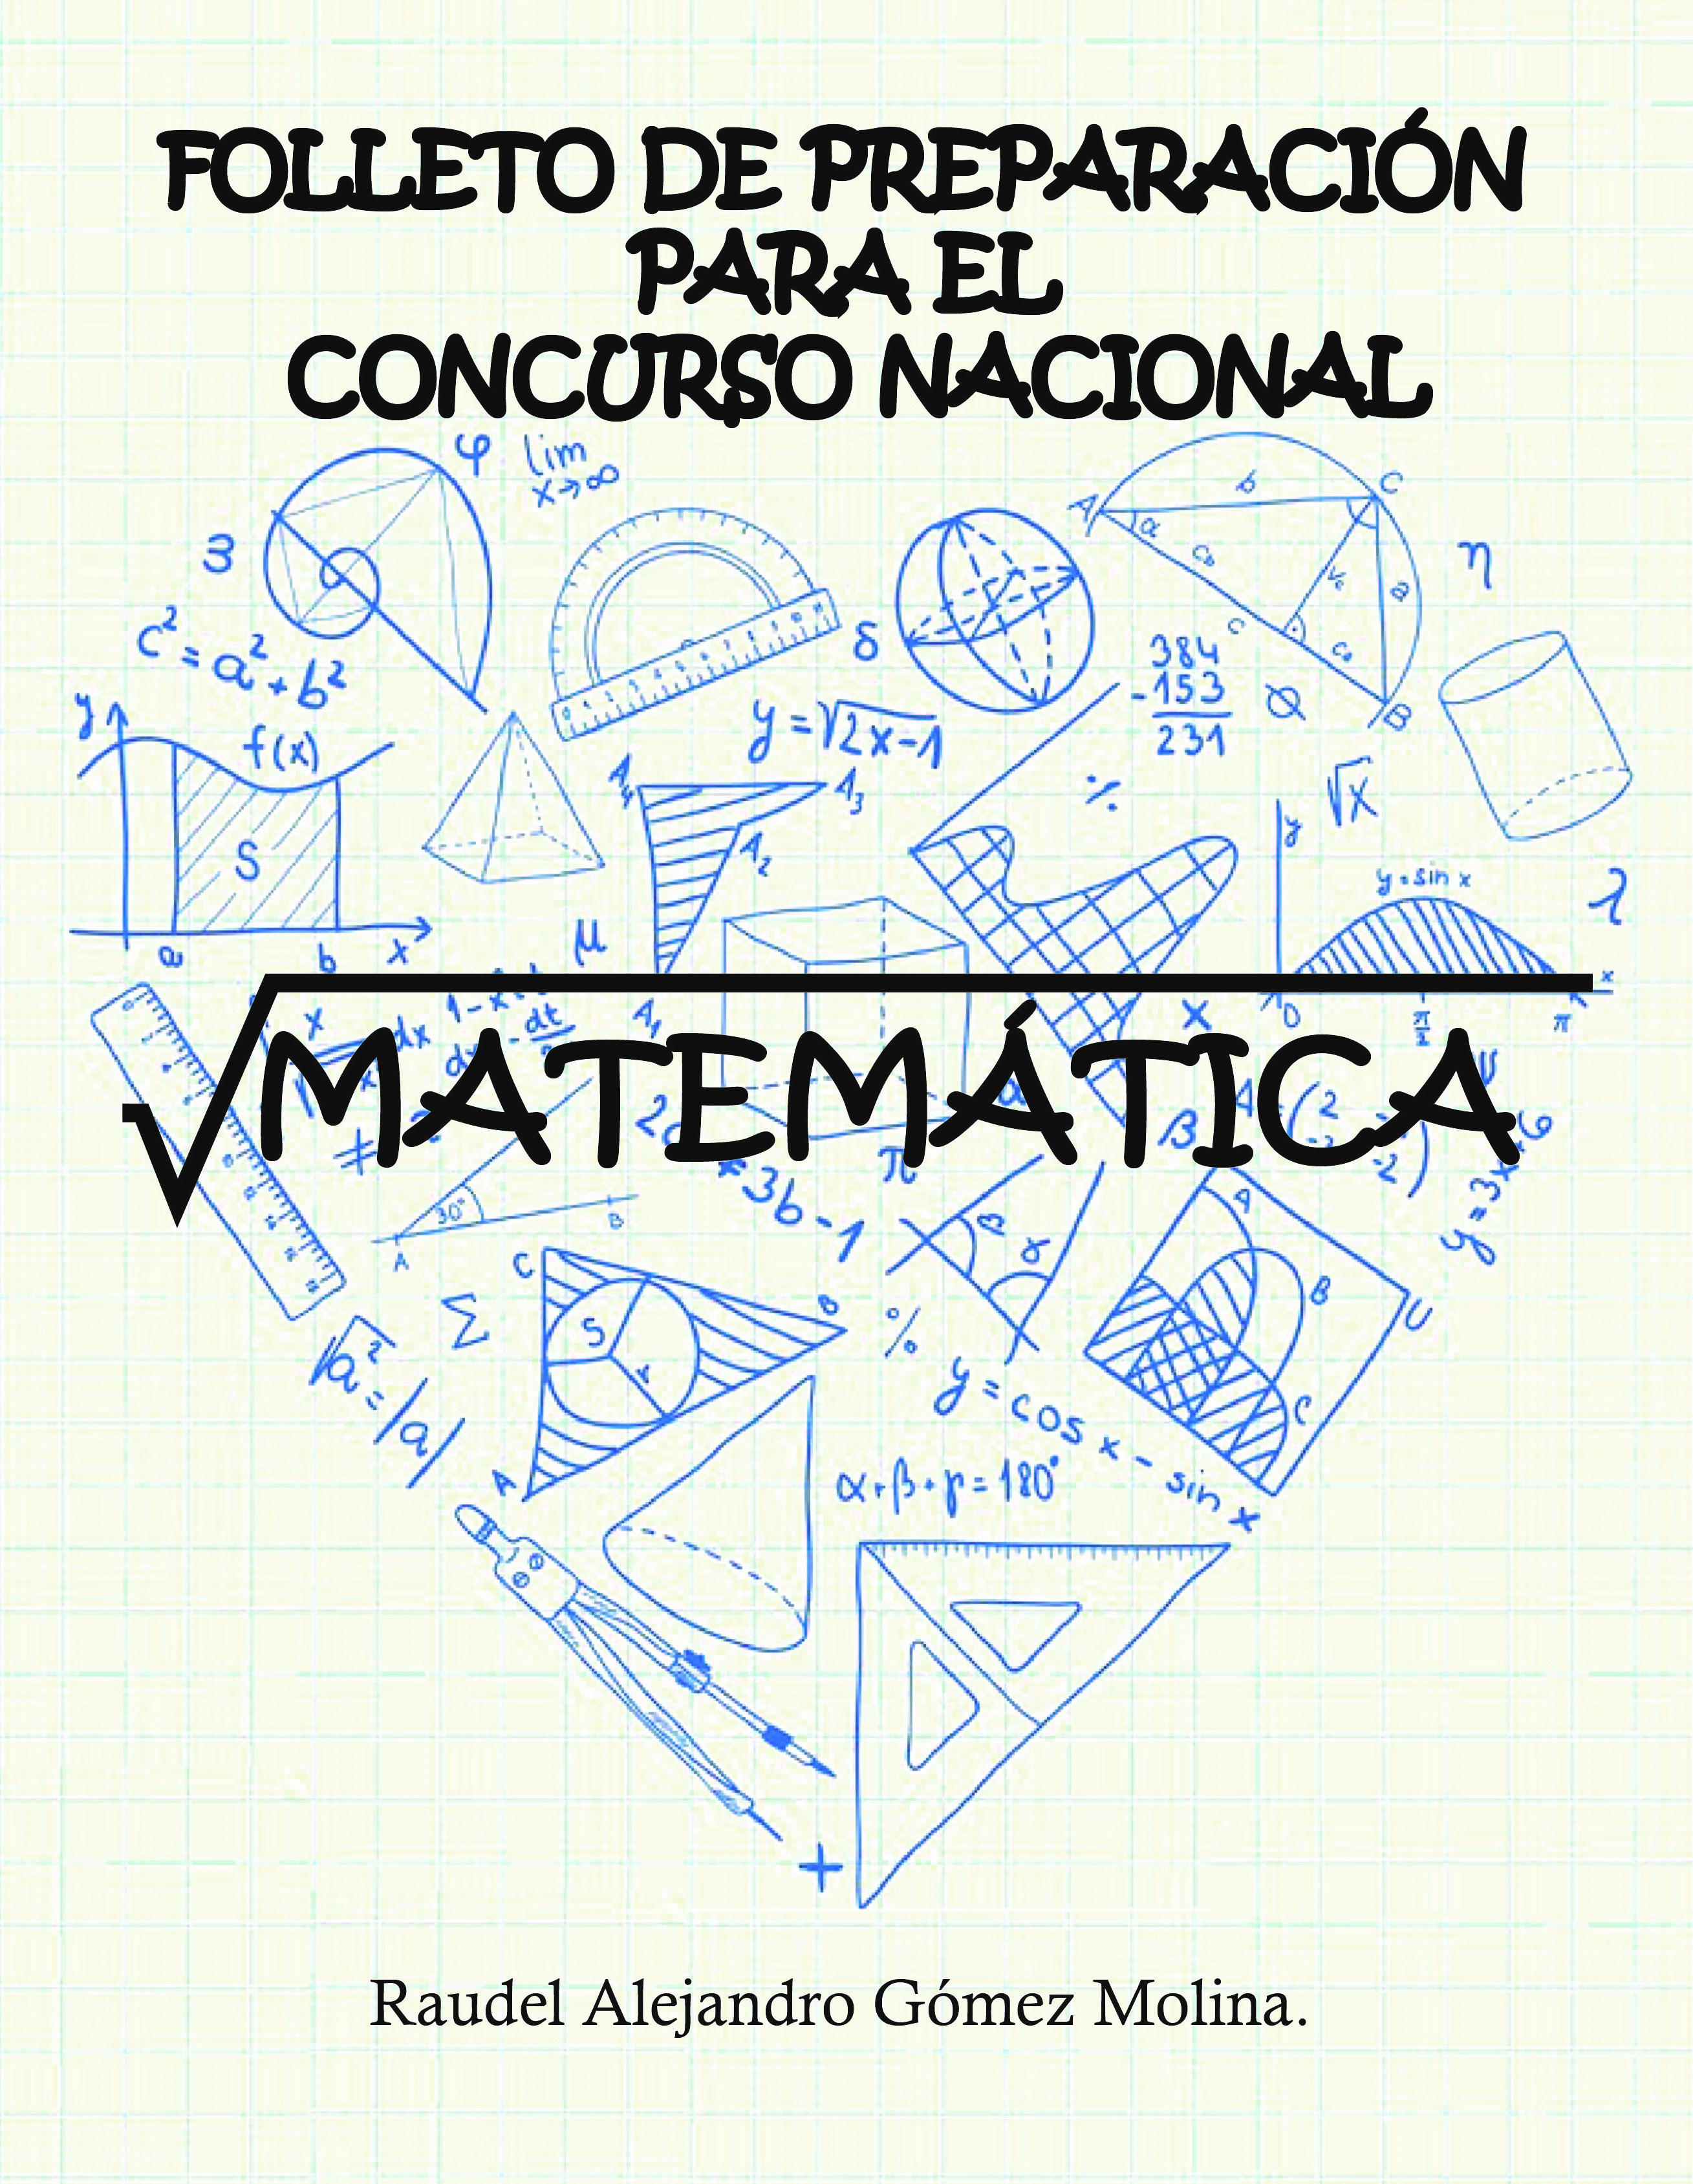
\includepdf[pages=-]{f.jpg}
\tableofcontents


\chapter{Teoría de Números}


\section{Ejercicios (Teoría de Números)}
\begin{enumerate}
    \item Diremos que un número entero positivo es exquisito, si es múltiplo del número de sus divisores.
          \begin{enumerate}
              \item  Hallar el mayor número exquisito de dos cifras.
              \item Pruebe que no existe un número exquisito cuyo último digito es 3.
          \end{enumerate}
    \item  Para todo $n$ entero positivo, sea $D(n)$ el número de divisores enteros positivos de $n$. Encuentre todos los enteros positivos $n$ para los cuales:
          \begin{enumerate}
              \item $n$ es múltiplo de 7.
              \item $n$ tiene al menos 4 factores primos.
              \item $2D(n)={[D(D(n))]}^2$ y este número divide a $n$.
              \item  $D_{(n)}= p^qq^p$ para dos primos $ p \neq q  $.
          \end{enumerate}
    \item Determine los enteros positivos $n$ tal que el número $N$ sea entero donde:
          $$N=\frac{2\cdot1}{\sqrt{1^2+1+4}+\sqrt{1^2-1+4}}+\frac{2\cdot2}{\sqrt{2^2+2+4}+\sqrt{2^2-2+4}}+ \ldots+                                \frac{2\cdot n}{\sqrt{n^2+n+4}+\sqrt{n^2-n+4}}$$
    \item Resolver en enteros $(a+1)(b-1)=a^2b^2$
    \item La sucesión $a_n$ está definida por $a_1 = 0$ y para todo $n\geq 1$:
          $$2a_n+1 = 5a_n + \sqrt{21{a_n}^2 + 4}$$
          Demostrar que todos los términos de la sucesión son enteros y determinar los valores de $n$ para los cuales $a_n$                       es divisible por 15.
    \item Determinar todos los primos $p,q,r,k$ tales que $pq+qr+rp= 12k + 1$.
    \item Si el entero $n^2 + 11$ es primo, probar que $n + 4$ no puede ser un cubo perfecto.
    \item Halle todas las parejas de enteros positivos $(m,n)$ tales que $m$ tiene dos dígitos, $n$ tiene tres dígitos, $m$ y                    $n$ tienen el mismo dígito de las unidades y $p$ es un número primo donde:
          $$p=\frac{mn}{m+n}$$
    \item Halle todos los primos $p,q$ tales que ${(p+q)}^2 = p^3+q^5$
    \item Sean $a,b\in \Z$ tales que $a-b=5b^2+4a^2$ demuestre que $a-b$ es un cuadrado perfecto.
    \item Decimos que un entero positivo $N$ es matedelicioso si existen tres divisores positivos distintos $a,b,c$ de $N$ tales que $N = a^2 + b^2 + c^2$.
          \begin{enumerate}
              \item Demuestre que existen a lo sumo 33 números matedeliciosos menores que 100.
              \item Demuestre que existen infinitos números matedeliciosos.
          \end{enumerate}
    \item Sean $a,b,c,d$ números reales tales que $a-b+c-d$ es impar y divide a $a^2-b^2+c^2-d^2$. Demuestre que
          $a-b+c-d$ divide a $a^n-b^n+c^n-d^n$ para todo entero positivo $n$.
    \item Encuentre todos los enteros positivos $a,b$ tales que $ab^2+b+7$ divide a $a^2b+a+b$.
    \item Encuentra todos los enteros positivos $a,b$ tal que los números
          \begin{center}
              $\displaystyle\frac{a^2b+a}{a^2+b}$ y $\displaystyle\frac{ab^2+b}{b^2-a}$
          \end{center}
          Son enteros.
    \item Encuentra para cuales enteros positivos $a,b$ es entera la fracción:
          $$\frac{b^2+a+b-1}{a^2+a+b+1}$$
          Es entera.
    \item Resuelva en enteros $3^x+4^y=5^z$
    \item Resolver en enteros no negativos: $7^a=4^b+5^c+6^d$
    \item Resolver en enteros positivos con $p$ primo: $x^2-3xy+p^2y^2=12p$
    \item Determina todos los pares de números naturales $(x,y)$ para los cuales se cumple que $x^2=4y+3mcm(x,y)$
    \item Resolver en enteros positivos: $x^2(x^2+y)=y^{m+1}$
    \item Determine todos los primos $p,q,r$ tales que: $p$ | $2qr+r$, $q$ | $2pr+p$ y $r$ | $2pq+q$.
    \item Encuentre todos los enteros positivos $n$ tales que:$2^n+n^2$ es un cuadrado perfecto.
    \item Encuentre todos los $n,k,p$ con $p$ primo tales que:
          $$n^5+n^4+1=p^k$$
    \item Sean $d_1<d_2< \ldots  <d_k$  los divisores positivos de $n$ . Encuentre todos los enteros positivos $k$  tales que                        $n=d_2d_3+d_2d_5+d_5d_3$.
    \item Pruebe que si $m,n$  y $r$  son enteros positivos, no nulos, que satisfacen que:
          $$m+1+n\sqrt{3}={\big(2+\sqrt{3}\big)}^{2r-1}$$
\end{enumerate}
\newpage


\section{Soluciones (Teoría de Números)}
\begin{enumerate}
    \item Diremos que un número entero positivo es exquisito, si es múltiplo del número de sus divisores.
          
          \begin{enumerate}
              \item  Hallar el mayor número exquisito de dos cifras.
              \item Pruebe que no existe un número exquisito cuyo último digito es 3.
          \end{enumerate}
          Respuesta:
          \begin{enumerate}
              \item Probemos con los números más grandes de dos cifras:\\
                    99$\rightarrow$4 divisores.\\
                    98$\rightarrow$4 divisores.\\
                    97$\rightarrow$2 divisores.\\
                    96$\rightarrow$12 divisores.\\
                    $ \therefore$ De aquí se concluye que el mayor número de dos cifras exquisito es 96 $\blacksquare$
              \item  Como el número termina en 3 el número de sus divisores debe ser impar y los únicos números que tienen un número de divisores impar son los cuadrados perfectos. \\
                    $\therefore$ No existe ningún cuadrado perfecto que termine en 3 $\blacksquare$ \\
          \end{enumerate}
    \item  Para todo $n$ entero positivo, sea $D(n)$ el número de divisores enteros positivos de $n$. Encuentre todos los enteros positivos $n$ para los cuales:
          \begin{enumerate}
              \item $n$ es múltiplo de 7.
              \item $n$ tiene al menos 4 factores primos.
              \item $2D(n)={[D(D(n))]}^2$ y este número divide a $n$.
              \item  $D_{(n)}= p^qq^p$ para dos primos $ p \neq q  $.
          \end{enumerate}
          Respuesta:\\
          Se tiene que:
          $$2p^qq^p = {[D(p^qq^p)]}^2$$
          $$2 p^qq^p = {(p + 1)}^2{(q + 1)}^2$$
          Entonces tenemos que $2 p^qq^p$ es un cuadrado perfecto esto implica que uno de los dos primos es igual a 2 ya que este aparece como factor lineal. Por lo tanto digamos sin pérdida de la generalidad que $p= 2$.
          $$\Rightarrow 2^{q+1}q^2 = 3^2(q + 1)^2$$
          Pero como $mcd(q;q + 1) = 1 \Rightarrow q = 3$, luego $D(n) = 72$. Entonces $n = 2^a3^b7^cm^d$ con $a,b,c,d$ enteros, $a \geq 3 ,b\geq  2$ y $m$ primo, porque $n$ no puede tener 5 factores primos diferentes, ya que los únicos 5 números que multiplicados dan 72 son:$2\cdot 2\cdot 2\cdot 3\cdot 3$ y uno de los exponentes debe ser mayor que 3. \\
          Pero $(a + 1)(b + 1)(c + 1)(d + 1) = 72$. Ahora busquemos los divisores de 72 mayores que 4 y veamos las posibilidades para $a + 1$.\\
          Para $a + 1 = 4$ se tiene que:
          $$(b + 1)(c + 1)(d + 1) = 18 \Rightarrow b + 1 = 3,c + 1 = 3,d + 1 = 2
              \vee  b + 1 = 3,c + 1 = 2,d + 1 = 3$$
          Para $a + 1 = 6$ se tiene que:
          $$(b + 1)(c + 1)(d + 1) = 12 \Rightarrow b + 1 = 3,c + 1 = 2,d + 1 = 2$$
          Para $a + 1 = 8$ se tiene que:\\
          $(b + 1)(c + 1)(d + 1) = 9$ imposible 9 no puede ser expresado como el producto de 3 enteros.\\
          Para $a + 1 = 9$ se tiene que: \\
          $(b + 1)(c + 1)(d + 1) = 8 \Rightarrow b + 1 = c + 1 = d + 1 = 2$  imposible porque $b + 1 \geq 3$. \\
          Para $a + 1 = 12$ se tiene que: \\
          $(b + 1)(c + 1)(d + 1) = 6$ imposible 6 no puede ser expresado como el producto de 3 enteros. \\
          Para $a + 1 = 18$ se tiene que: \\
          $(b + 1)(c + 1)(d + 1) = 4$ imposible 4 no puede ser expresado como el producto de 3 enteros.\\
          Para $a + 1 = 24$ se tiene que: \\
          $(b + 1)(c + 1)(d + 1) = 3$ imposible 3 no puede ser expresado como el producto de 3 enteros.\\
          Para $a + 1 = 36$ se tiene que: \\
          $(b + 1)(c + 1)(d + 1) = 2$ imposible 2 no puede ser expresado como el producto de 3 enteros.\\
          Para $a + 1 = 72$ se tiene que: \\
          $(b + 1)(c + 1)(d + 1) = 1$ imposible 1 no puede ser expresado como el producto de 3 enteros. \\
          $\therefore$ Las soluciones son $n= 2^33^27^2m , n= 2^33^27m^2, n= 2^53^27m$ $\blacksquare$\\
    \item Determine los enteros positivos $n$ tal que el número $N$ sea entero donde:
          $$N=\frac{2\cdot1}{\sqrt{1^2+1+4}+\sqrt{1^2-1+4}}+\frac{2\cdot2}{\sqrt{2^2+2+4}+\sqrt{2^2-2+4}}+ \ldots+                                \frac{2\cdot n}{\sqrt{n^2+n+4}+\sqrt{n^2-n+4}}$$
          Respuesta:\\
          Racionalicemos el último sumando:
          $$\frac{2\cdot n}{\sqrt{n^2+n+4}+\sqrt{n^2-n+4}}=\frac{2\cdot n}{\sqrt{n^2+n+4}+\sqrt{n^2-n+4}}\cdot\frac{\sqrt{n^2+n+4}-\sqrt{n^2-n+4}}{\sqrt{n^2+n+4}-\sqrt{n^2-n+4}}$$
          $$\frac{2\cdot n}{\sqrt{n^2+n+4}+\sqrt{n^2-n+4}}=\frac{2n\big(\sqrt{n^2+n+4}-\sqrt{n^2-n+4}\big)}{n^2+n+4-n^2-n+4}$$
          $$\frac{2\cdot n}{\sqrt{n^2+n+4}+\sqrt{n^2-n+4}}=\frac{2n\big(\sqrt{n^2+n+4}-\sqrt{n^2-n+4}\big)}{2n}$$
          $$\frac{2\cdot n}{\sqrt{n^2+n+4}+\sqrt{n^2-n+4}}=\sqrt{n^2+n+4}-\sqrt{n^2-n+4}$$
          De manera análoga se tiene que:
          $$N=\sqrt{1^2+1+4}-\sqrt{1^2-1+4}+\ldots+\sqrt{{(n-1)}^2+n-1+4}-        \sqrt{{(n-1)}^2-n+1+4}+\sqrt{n^2+n+4}-\sqrt{n^2-n+4}$$
          $$N=\sqrt{1^2+1+4}-\sqrt{1^2-1+4}+\ldots+\sqrt{n^2-2n+1+n-1+4}-\sqrt{n^2-2n+1-n+1+4}+\sqrt{n^2+n+4}-\sqrt{n^2-n+4}$$
          $$N=\sqrt{1^2+1+4}-\sqrt{1^2-1+4}+\ldots+\sqrt{n^2-n+4}-\sqrt{n^2-3n+5}+\sqrt{n^2+n+4}-\sqrt{n^2-n+4}$$
          Así se van cancelando telescópicamente:
          $$N= \sqrt{n^2+n+4} - 2$$
          $$\Rightarrow n^2 + n + 4 = b^2$$
          con $b \in \Z$ \\
          Claramente una solución es $n = 0$. \\Ahora:
          $$n^2\leq n^2 + n + 4 \leq {(n+2)}^2$$
          $$\Rightarrow  n^2 + n + 4 ={(n+1)}^2$$
          $$n^2 + n + 4=n^2+2n+1$$
          $$n=3$$
          $\therefore$ Las soluciones son $n = 3$ y $n = 0$ $\blacksquare$\\
    \item  Resolver en enteros $(a+1)(b-1)=a^2b^2$\\
          Respuesta:\\
          Nótese que $mcd[(a + 1);a] = mcd[(b - 1);b] = 1 \Rightarrow b - 1 = a^2 \wedge a + 1 = b^2$\\
          Despejando y sustituyendo se tiene que:
          $$a + 1 = a^4 + 2a^2 + 1$$
          $$a(a^3 + 2a - 1) = 0 \Rightarrow a = 0$$
          Las demás soluciones no son enteras. Falta considerar cuando $b= 0$\\
          $\therefore$ Las soluciones son $a= 0 \; b= 1, b= 0\; a= -1$ $\blacksquare$\\
    \item La sucesión $a_n$ está definida por $a_1 = 0$ y para todo $n\geq 1$:
          $$2a_n+1 = 5a_n + \sqrt{21{a_n}^2 + 4}$$
          Demostrar que todos los términos de la sucesión son enteros y determinar los valores de $n$ para los cuales $a_n$                       es divisible por 15.\\
          Repuesta:
          $$2a_{n+1} - 5a_n = \sqrt{21{a_n}^2 + 4}$$
          $${(4a_n+1)}^2 - 20a_{n+1}a_n + 25{a_n}^2 = 21{a_n}^2 + 4$$
          $$(1)\; {a_{n+1}}^2 - 5a_{n+1}a_n + {a_n}^2 = 1$$
          Sustituyamos  $n$ por $n - 1$ :
          $$(2)\;{a_n}^2 - 5a_n a_{n-1} + {a_{n-1}}^2 = 1$$
          Restemos (1) y (2) :
          $$a_n+12 - a_n-12 - 5a_{n+1}a_n + 5a_na_{n-1} = 0$$
          $$(a_{n+1} - a_{n-1})(a_{n+1} + a_{n-1} - 5a_n) = 0$$
          Pero como $a_{n+1} - a_{n-1} \neq 0$ ya que la sucesión sería constante.
          $$\Rightarrow a_{n+1} + a_{n-1} - 5a_n = 0$$
          De aquí se concluye que todos los términos de la sucesión son enteros.\\
          Aplicando congruencia módulo 5 queda que:
          \begin{center}
              $a_{n+1} \equiv a_{n-1}$(mód 5)
          \end{center}
          Pero como $a_1 = 0$ y $a_2 = 1$ se concluye que:
          \begin{center}
              $a_{2k} \equiv 1$(mód 5) y $a_{2k+1} \equiv 0$(mód 5)
          \end{center}
          Aplicando congruencia módulo 3 queda que:
          \begin{center}
              $a_{n+1} + a_{n-1} + a_n \equiv 0$(mód 3)
          \end{center}
          Pero como $a_3 \equiv 2$(mód 3) se concluye que: $a_{3k+1} \equiv 0$(mód 3),  $a_{3k+2} \equiv 1$(mód 3) y  $a_{3k+3} \equiv 2$(mód 3). \\
          $\therefore$ Para $n = 6k + 1$, $a_n$ es divisible por 15 $\blacksquare$\\
    \item Determinar todos los primos $p,q,r,k$ tales que $pq+qr+rp= 12k + 1$.\\
          Respuesta:\\
          Supongamos que $p,q,r,k$ son diferentes de 2 y 3. Entonces dejan resto 1 ó - 1 en el módulo 4 y en el módulo 3 . Se nos presentan los siguientes casos:
          \begin{center}
              $1 \cdot 1 + 1 \cdot 1 + 1 \cdot 1 \equiv 1$(mód 3) \\
              $-1 \cdot 1 + (-1) \cdot 1 + 1 \cdot 1 \equiv 1$(mód 3)\\
              $-1 \cdot (-1) + 1 \cdot (-1) + 1 \cdot (-1) \equiv 1$(mód 3)\\
              $1 \cdot 1 + 1 \cdot 1 + 1 \cdot 1 \equiv 1$(mód 4)\\
              $-1 \cdot 1 + (-1) \cdot 1 + 1 \cdot 1 \equiv 1$(mód 4) \\
              $-1 \cdot (-1) + 1 \cdot (-1) + 1 \cdot (-1) \equiv 1$(mód 4) \\
          \end{center}
          Las demás posibilidades se obtienen de permutar estas expresiones. Ahora todos estos casos nos arrojan contradicciones eso implica uno es 2 y otro es 3.\\
          Sin pérdida de la generalidad digamos que $p= 2$ y $q= 3$ $\Rightarrow$ $2r + 3r + 6 = 12k + 1$
          $$5r + 5 = 12k \Rightarrow k = 5 \wedge r= 11$$
          $\therefore$ Las soluciones son $p= 2, q= 3, r= 11$ y sus permutaciones con $k= 5$ $\blacksquare$ \\
    \item Si el entero $n^2 + 11$ es primo, probar que $n + 4$ no puede ser un cubo perfecto.\\
          Respuesta:\\
          Digamos que $n + 4 \Rightarrow k^3\Rightarrow n = k^3 - 4$. Sustituyendo nos queda que:
          $$\big(k^3 - 4\big)^2 + 11 = k^6 - 8k^3 + 27$$
          $$\big(k^3 - 4\big)^2 + 11 = k^6 - 9k^3 + k^3 + 27$$
          $$\big(k^3 - 4\big)^2 + 11 = \big(k^2\big)^3 + 3^3 + k^3 - 3 \cdot 3k^2k$$
          Que se factoriza de acuerdo a la identidad:
          $$a^3 + b^3 + c^3 - 3abc = (a + b + c)(a^2 + b^2 + c^2 - ab - bc - ca)$$
          $$\big(k^3 - 4\big)^2 + 11 = \big(k^2 + k + 3\big)\big(\big(k^2\big)^2 + k^2 + 3^2 - 3k - 3k^2 - k^2k\big)$$
          Lo cual es una contradicción. \\
          $\therefore$ Queda demostrado que $n + 4$ no puede ser un cubo perfecto $\blacksquare$\\
    \item  Halle todas las parejas de enteros positivos $(m,n)$ tales que $m$ tiene dos dígitos, $n$ tiene tres dígitos, $m$ y                    $n$ tienen el mismo dígito de las unidades y $p$ es un número primo donde:
          $$p=\frac{mn}{m+n}$$
          Respuesta:\\
          Digamos que $mcd(m;n) = d, m = ad$ y $n = bd$ con $mcd(b;a) = 1$:
          $$adp + bdp = abd^2$$
          $$ap + bp = abd$$
          $$\Rightarrow a |bp    \wedge   b| ap $$
          $$\Rightarrow a| p    \wedge   b |p $$
          porque $mcd(b;a) =1$. \\
          Suponiendo que $a$ y $b$ son diferentes de uno.
          $$\Rightarrow a=b=p$$
          Lo cual es absurdo ya que $n > m \Rightarrow a = 1 \wedge b=p$. $\Rightarrow                b + b^2 = bd$
          $\Rightarrow b + 1 = d$ Luego $m = b + 1$ y $n = b(b + 1)$. Ahora $b^2 + b                        \geq 100 \Rightarrow b \geq 10$. Pero además tenemos que:
          \begin{center}
              $b^2 + b \equiv b + 1$(mód 10)\\
              $b^2 \equiv 1$(mód 10)\\
              $b \equiv 1 \vee 9$(mód 10)\\
          \end{center}
          Para $b= 11 \Rightarrow m = 12 \wedge n = 132$. \\
          Para $b = 19 \Rightarrow m = 20 \wedge n = 380$. \\
          Para $b = 29 \Rightarrow m = 30 \wedge n = 870$. \\
          Para $b = 31 \Rightarrow m = 32 \wedge n = 992$. \\
          Para $ b = 41 \Rightarrow m= 42 \wedge n = 1772$ pero $n > 1000$ lo cual es imposible. \\
          $\therefore$ Las soluciones son $m= 12$ y $n= 132$, $m= 20$ y $n= 380$, $m= 30$ y $n= 870$ y $m= 32$ y $n= 992$ $\blacksquare$\\
    \item Halle todos los primos $p,q$ tales que ${(p+q)}^2 = p^3+q^5$ \\
          Respuesta:\\
          Supongamos que $p$,$q$ son distintos de 3.
          \begin{center}
              $p\equiv 1 \vee -1$(mód 3)  y $q\equiv 1 \vee -1$(mód 3)
          \end{center}
          Para $p\equiv 1$(mód 3)  y $q\equiv 1 $(mód 3):
          \begin{center}
              $1\equiv 1-1$(mód 3)
          \end{center}
          Para $p\equiv 1 $(mód 3)  y $q\equiv -1 $(mód 3):
          \begin{center}
              $0\equiv 1+1$(mód 3)
          \end{center}
          Para $p\equiv -1 $(mód 3)  y $q\equiv 1 $(mód 3):
          \begin{center}
              $0\equiv -1-1$(mód 3)
          \end{center}
          Para $p\equiv -1 $(mód 3)  y $q\equiv -1 $(mód 3):
          \begin{center}
              $1\equiv -1+1$(mód 3)
          \end{center}
          Todos los casos arrojan contradicciones esto nos dice que $p=3$ ó  $q=3$.
          Para $q=3$:
          $$p^2+6p+9=p^3-243 \Rightarrow p=7$$
          Para $p=3$:
          $$q^2+6q+9=27-q^5 $$  no tiene soluciones enteras.\\
          $\therefore$ Las soluciones son $p=7$ y $q=3$ $\blacksquare$\\
          
          
    \item Sean $a,b\in \Z$ tales que $a-b=5b^2+4a^2$ demuestre que $a-b$ es un cuadrado perfecto.\\
          Respuesta:\\
          Factoricemos:
          $$a - b + 4(a - b)(a + b) = b^2$$
          $$(a-b)(1 + 4a + 4b) = b^2$$
          Digamos que $mcd(a;b) = d$, $a = a_1d$ y $b = b_1d$ con $mcd(a_1;b_1) = 1$.                    $$(a_1d - b_1d)(1 + 4a_1d + 4b_1d) = (b_1d)^2$$
          $$(a_1 - b_1)(1 + 4a_1d + 4b_1d) = (b_1)^2d$$
          Pero $mcd(1 + 4a_1d + 4b_1d;d) = 1$ y $mcd(a)1 - b_1;b_1) = 1$
          $$\Rightarrow 1 + 4a_1d + 4b_1d = (b_1)^2 \wedge a_1 - b_1 = d$$
          $\therefore (a_1 - b_1)d = a - b \Rightarrow d^2 = a - b$ $\blacksquare$ \\
    \item Decimos que un entero positivo $N$ es matedelicioso si existen tres divisores positivos distintos $a,b,c$ de $N$ tales que $N = a^2 + b^2 + c^2$.
          \begin{enumerate}
              \item Demuestre que existen a lo sumo 33 números matedeliciosos menores que 100.
              \item Demuestre que existen infinitos números matedeliciosos.
          \end{enumerate}
          Respuesta:\\
          Supongamos que $N$ no es múltiplo de 3. Luego esto implica que ninguno de sus divisores es múltiplo de 3:
          \begin{center}
              $N\equiv a^2 + b^2 + c^2$ (mód 3)
              $N\equiv  1 + 1 + 1$ (mód 3)
          \end{center}
          Por lo que hemos llegado a una contradicción. Luego $N$ es múltiplo de 3 y sólo hay 33 múltiplos de 3 menores que 100. Por otro lado tenemos que $30 = 1^2 + 2^2 + 5^2$ luego tomemos el número: $30k^2$ se cumple que $k,2k$ y $5k$ son divisores de este número y además se cumple que: $30k^2 = 1^2k^2 + 2^2k^2 + 5^2k^2$.\\
          $\therefore$ Quedan demostrados los dos incisos $\blacksquare$ \\
    \item Sean $a,b,c,d$ números reales tales que $a-b+c-d$ es impar y divide a $a^2-b^2+c^2-d^2$. Demuestre que
          $a-b+c-d$ divide a $a^n-b^n+c^n-d^n$ para todo entero positivo $n$.\\
          Respuesta:\\
          Nótese que:
          $$a-b + c-d| (a + c - b - d)(a + b + c + d)$$
          $$ \Rightarrow a-b + c-d |(a+ c)^2 - (b + d)^2 $$
          $$a-b+ c-d |a^2 + 2ac + c^2 - b^2 - 2bd - d^2$$
          $$ \Rightarrow a-b + c-d| 2(ac - bd)$$
          Luego   $\Rightarrow a-b + c-d|(ac + bd) $  porque $a-b + c-d$ es impar. \\
          Tomemos $n= 1$ y $n= 2$ como inicio de inducción:
          $$a-b + c-d| a-b +c-d $$
          $$a-b +c-d |a^2  -b^2 + c^2 - d^2$$
          Supongamos hasta  $n=k$ y demostremos para $n=k + 1$:
          $$a-b + c-d| (a + c)(a^n + c^n) - (a+ c)(b^n + d^n)$$
          Pero se cumple que:
          $$a-b + c-d |(a + c - b - d)(b^n + d^n)$$
          $$\Rightarrow a-b + c-d |(a + c)(a^n + c^n) - (a + c)(b^n + d^n) + (a + c - b -d)(b^n + d^n)$$
          $$a-b + c-d| (a + c)(a^n + c^n) - (b + d)(b^n + d^n)$$
          $$a-b + c-d |a^{n+1} - b^{n+1} + c^{n+1} - d^{n+1} + ca^n + ac^n - bd^n - db^n$$
          $$a-b + c-d| a^{n+1} - b^{n+1} + c^{n+1} - d^{n+1} + ac(a^{n-1} + c^{n-1}) -bd(d^{n-1} + b^{n-1})$$
          Pero se cumple que:
          $$a-b + c-d| (ac - bd)(a^{n-1} + c^{n-1})$$
          $$\Rightarrow a-b + c-d| a^{n+1} - b^{n+1} + c^{n+1} - d^{n+1} + ac(a^{n-1} + c^{n-1}) - bd(d^{n-1} + b^{n-1}) -(ac - bd)(a^{n-1} + c^{n-1})$$
          $$a-b + c-d| a^{n+1} - b^{n+1} + c^{n+1} - d^{n+1} + bd(a^{n-1} + c^{n-1} - d^{n-1} - b^{n-1})$$
          Pero por hipótesis de inducción:
          $$a-b + c-d| (a^{n-1} + c^{n-1} - d^{n-1} - b^{n-1})$$
          $$\Rightarrow a-b + c-d| a^{n+1} - b^{n+1} + c^{n+1} - d^{n+1}$$
          $\therefore$ Se cumple que:  $a-b + c-d| a^n - b^n + c^n - d^n $   para todo  $n$  entero $\blacksquare$\\
    \item Encuentre todos los enteros positivos $a,b$ tales que $ab^2+b+7$ divide a $a^2b+a+b$.\\
          
          Respuesta:\\
          Nótese que:
          $$ab^2 + b + 7| (a^2b + a + b)b - (ab^2 + b + 7)a$$
          $$ \Rightarrow ab^2 + b + 7 |b^2 - 7a$$
          $$\Rightarrow |b^2 7a| \geq ab^2 + b + 7 $$
          $$\Rightarrow (1)\;b^2 - 7a \geq ab^2 + b + 7      \vee   (2)\; - (b^2 - 7a) \geq ab^2 + b + 7 $$
          $$(1)\; - 7a \geq ab^2 - b^2 + b + 7$$
          Pero $ab^2 \geq b^2$ por lo tanto: $ab^2 -b^2 + b + 7 \geq 0 \Rightarrow 0 \geq a$ lo cual es una contradicción.
          $$(2)\; - (b^2 - 7a) \geq ab^2 + b + 7$$
          $$ 7a - ab^2 \geq b^2 + b + 7 \geq 0$$
          $$ 7a \geq ab^2$$
          $$7 \geq b^2$$
          Entonces se nos presentan los siguientes casos $b= 1$ y $b= 2$
          Para $b= 1$:
          $$a + 8| 7a - 1$$
          $$a + 8| 7a + 56 - 57$$
          $$\Rightarrow a + 8| -57 \Rightarrow a= 49\vee a= -7 $$
          porque 57 es primo
          Para $b= 2$:
          $$4a + 9| 7a- 4$$
          
          $$\Rightarrow 4a + 9 |3a- 13$$
          $$ \Rightarrow a- 13 \geq 4a + 9$$
          $$-22 \geq a $$
          Lo cual es una contradicción
          $\therefore$ Las soluciones son $a= 49$ y $   b = 1$ $\blacksquare$  \\
    \item Encuentra todos los enteros positivos $a,b$ tal que los números
          \begin{center}
              $\displaystyle\frac{a^2b+a}{a^2+b}$ y $\displaystyle\frac{ab^2+b}{b^2-a}$
          \end{center}
          Son enteros.\\
          Respuesta:\\
          Se cumple que:
          $$a^2 + b |a^2b + a\wedge b^2 - a| b^2a+ b $$
          $$ \Rightarrow a^2 + b| a^2b + a - a^2b - b^2 \wedge b^2 -a| b^2a + b - b^2a + a^2 $$
          $$ \Rightarrow a^2 + b| -(b^2 - a)  \wedge  b^2 - a |a^2 + b $$
          $$\Rightarrow a^2 + b = \pm(b^2 - a)$$
          Para $a^2 + b = b^2 - a$ se tiene que:
          $$(a + b)(a - b + 1) = 0$$
          $$\Rightarrow a=-b \vee a = b- 1$$
          Para $a^2 + b = -b^2 + a $ se tiene que:
          $$a^2 -a = -b^2 -b$$
          Como los números son enteros positivos eso significa que el MI es negativo.
          $$\Rightarrow a^2 \leq a$$
          $$\Rightarrow a= 1  \vee a= 0$$
          Pero como son enteros positivos las soluciones son:  $a= 1$  y $a= b- 1$
          Para $a= 1$ se tiene que:
          $$\frac{b + 1}{1 + b}=1$$
          $$\frac{b^2 + b}{b^2 - 1} =\frac{b}{b-1}$$
          Esto implica que $b= 2$ porque $mcd(b;b-1) = 1$ \\
          Para $a + 1 =b$ se tiene que:
          $$\frac{a^2(a + 1) + a}{ a^2 + a + 1}=a $$
          $$\frac{{(a + 1)}^2 a + a + 1}{{(a + 1)}^2 - a}=\frac{a^3 + 2a^2 + 2a + 1}{ a^2 + a + 1}= a + 1$$
          $\therefore$ Las soluciones son $a + 1 =b$ y $a$ para todo entero $a$ y $a= 1$ y $b= 2$ $\blacksquare$ \\
    \item  Encuentra para cuales enteros positivos $a,b$ es entera la fracción:
          $$\frac{b^2+a+b-1}{a^2+a+b+1}$$
          Es entera.\\
          Respuesta:\\
          Tenemos que: $$a^2 + ab + 1| b^2 + ab + a + b - 1$$
          $$\Rightarrow a^2 + ab + 1| b^2 + ab + a + b - 1 + a^2 + ab + 1 $$
          $$\Rightarrow a(a + b) + 1 |{(a + b)}^2 + a + b$$
          $$a(a + b) + 1| (a + b)(a + b + 1)$$
          Pero $mcd(a(a + b) + 1;a + b) = 1$:
          $$a(a + b) + 1| a + b + 1 $$
          $$\Rightarrow a + b + 1 \geq (a + b)a + 1$$
          $$\Rightarrow a + b \geq (a + b)a$$
          $$\Rightarrow 1 \geq a$$
          $$\Rightarrow 1 = a $$
          Sustituyendo:
          $$b + 2| b^2 + 2b$$
          $$ b + 2 |b(b + 2)$$
          $\therefore$ Las soluciones son $a = 1$ y $b$ puede ser cualquier entero positivo $\blacksquare$\\
    \item Resuelva en enteros $3^x+4^y=5^z$.\\
          Respuesta:\\
          Trabajemos con los módulos 3 y 4:
          \begin{center}
              $4^y \equiv 5^z$(mód 3) \\
              $1^y \equiv (-1)^z$(mód 3)$ \Rightarrow z= 2c$\\
              $ 3^x \equiv 5^z$(mód 4)\\
              $ (-1)^x \equiv 1^z$(mód 4) $\Rightarrow x= 2a$\\
          \end{center}
          Entonces la ecuación nos queda así $3^{2a} + 2^{2y} = 5^{2c} $. Ahora estamos en presencia de un trío pitagórico primitivo, por tanto se cumple que:
          $$3^a = m^2 - n^2$$
          $$2^y = 2mn$$
          $$5^c = m^2 + n^2$$
          con $m$ y $n$ primos relativos y $m > n$.
          Como $2^y = 2mn$ implica que $m$ y $n$ son potencias de 2 y como son primos relativos $\Rightarrow m= 2^{y-1} \wedge n= 1$. \\
          $3^{2a} = (2y-1 + 1)(2y-1 - 1)$ por lo que los dos factores son potencias de 3 cuya diferencia es 2 y las únicas potencias que cumplen esto son 3 y 1 $\Rightarrow y= 2\wedge m= 2$.\\
          Solo nos falta considerar cuando $x=0$ y $y=0$.\\
          Para $x=0$ tenemos que:
          $$1+4^y=5^z$$
          $$1+4^y={(4+1)}^z$$
          $$1+4^y=4^z+{z\choose 1}4^{z-1}+ {z\choose 2}4^{z-2}+\ldots+4^1+1$$
          $$4^{y-1}=4^{z-1}+{z\choose 1}4^{z-2}+ {z\choose 2}4^{z-3}+\ldots+4+1$$
          $$\Rightarrow y=1\Rightarrow z=1$$
          Para $y=0$ tenemos que:
          $$3^x+1=5^z$$
          $$3^x=(5-1)(5^{z-1}+5^{z-2}+\ldots+5+1)$$
          lo cual es imposible.\\
          $\therefore$ Las soluciones son $x=y=z=2$ y $x=0$ y $y=z= 1$ $\blacksquare$ \\
    \item Resolver en enteros no negativos: $7^a=4^b+5^c+6^d$\\
          Respuesta:\\
          Analicemos las terminaciones:
          \begin{center}
              $7^a\equiv 7 ,9 ,3 ,1$ (mód 10)\\
              $4^b\equiv 4 ,6$ (mód 10)\\
              $5^c\equiv 5$ (mód 10)\\
              $6^d\equiv 6$ (mód 10)\\
          \end{center}
          Analicemos congruencia módulo 4:
          \begin{center}
              $3^a\equiv 4^b+1+2^d$  (mód 4)\\
          \end{center}
          Asumamos que $d\geq 2$:
          \begin{center}
              $3^a\equiv 4^b+1+0$ (mód 4)
          \end{center}
          $$\Rightarrow b>0 \wedge a=2k$$
          Analicemos la terminaciones:
          \begin{center}
              $9\equiv 4+5+6$ (mód 4)
              $9\equiv 6+5+6$ (mód 4)
              $1\equiv 4+5+6$ (mód 4)
              $1\equiv 6+5+6$ (mód 4)
          \end{center}
          Todos los casos arrojan contradicciones, luego $d<2$.\\
          Para $d=1$:\\
          Analicemos congruencia módulo 6:
          \begin{center}
              $$1\equiv{(-2)}^b+{(-1)}^c$$  (mód 6)\\
          \end{center}
          Demostremos que:
          \begin{center}
              $2^n\equiv 4$ (mód 6) para todo $n\geq2$.\\
          \end{center}
          Inicio de inducción $n=2$:
          \begin{center}
              $4\equiv 4$ (mód 6)\\
          \end{center}
          Supongamos para $n=k$:
          \begin{center}
              $2^k\equiv 4$ (mód 6)\\
          \end{center}
          Demostremos para $n=k+1$:
          \begin{center}
              $2^{(k+1})\equiv 2\cdot 2^k$  (mód 6)\\
              $2^{(k+1)}\equiv 2\cdot 4$ (mód 6)\\
              $2^{(k+1)}\equiv 4$ (mód 6)\\
          \end{center}
          Con lo cual queda demostrado.
          \begin{center}
              $\Rightarrow 1\equiv \pm 4+{(-1)}^c$  (mód 6)\\
          \end{center}
          Esto es una contradicción lo cual implica que $d=0$:\\
          $$7^a=4^b+5^c+1$$
          Analicemos las terminaciones:
          $$\Rightarrow b=0 \wedge a=4k+1$$
          $$7^a=1+5^c+1$$
          Demostremos que:
          \begin{center}
              $7^{(4k+1)}\equiv 7$ (mód 100)\\
          \end{center}
          Inicio de inducción $k=1$:
          \begin{center}
              $16807\equiv 7$ (mód 100)\\
          \end{center}
          Supongamos para $k=m$:
          \begin{center}
              $7^{(4m+1)}\equiv 7$ (mód 100)\\
          \end{center}
          Demostremos para $k=m+1$:
          \begin{center}
              $7^{(4m+5)}\equiv 2401\cdot 7^{(4m+1)}$  (mód 100)\\
              $7^{(4m+5)}\equiv 1\cdot 7$ (mód 100)\\
          \end{center}
          Con lo cual queda demostrado.\\
          Ahora si $c\geq 2\Rightarrow 5^c\equiv 25$ (mód 100). De aquí se deduce que $c=1$.\\
          $\therefore$ Las soluciones son $a=1$, $b=0$, $c=1$, y $c=0$ $\blacksquare$\\
    \item Resolver en enteros positivos con $p$ primo: $x^2-3xy+p^2y^2=12p$ \\
          Respuesta:\\
          Analicemos la congruencia módulo 3:
          \begin{center}
              $\Rightarrow x^2+p^2 y^2\equiv 0$ (mód 3)
          \end{center}
          Ahora supongamos que $p\neq3$:
          $$\Rightarrow x=3a \wedge y=3b$$
          con a y b enteros positivos. \\
          Sustituyendo:
          $${(9a)}^2-27ab+{(9p)}^2 a^2=12p$$
          $${(3a)}^2-9ab+{(3p)}^2 a^2=4p$$
          Esto nos dice que p es divisible entre 3, luego $p=3$ y lo que supusimos anteriormente fue falso.\\
          Sustituyendo $p=3$:
          $$x^2-3xy+9y^2=36$$
          De aquí se deduce que $x=3c$, con $c$ entero positivo.
          $${(9c)}^2-9cy+9y^2=36$$
          $$c^2-cy+y^2=4$$
          Fijemos $y$ y utilicemos el discriminante que tiene que ser un cuadrado perfecto.
          $$D=y^2-4y^2+16$$
          $$0\leq y^2-4y^2+16$$
          $${(3y)}^2\leq 16$$
          $$y^2\leq 4$$
          Para y=2:
          $$c^2-2c+4=4$$
          $\Rightarrow c=2 \wedge c=0$
          Para y=1:
          $$c^2-c-3=0$$
          No hay solución entera.\\
          Para y=0:
          $$c^2-4=0$$
          $$\Rightarrow c=2 \wedge c=-2$$
          $\therefore$ Las soluciones enteras positivas son: $y=0$, $x=6$ y $p=3$; $y=2$, $x=6$ y $p=3$ y $y=2$, $x=0$ y $p=3$ $\blacksquare$\\
    \item Determina todos los pares de números naturales $(x,y)$ para los cuales se cumple que $x^2=4y+3mcm(x,y)$\\
          Respuesta:\\
          Digamos que el $mcd(x,y)=d$,$x=ad$,$y=bd$ y $mcd(a,b)=1$ con $a,b,d$ naturales.
          $${(da)}^2  = 4db +3adb$$
          $$da^2  = 4b +3ab$$
          $$\Rightarrow a|4b \Rightarrow a=1,a=2 \vee a=4$$
          Para a=1:
          $$d = 7b\Rightarrow x=7b \wedge y=7b^2$$
          Para a=2:
          $$2d = 2b +3b$$
          Entonces $b$ es par pero entonces no se cumple que $mcd(a,b)=1$.\\
          Para a=4:
          $$4d =b+3b\Rightarrow d=b\Rightarrow x=4b \wedge y=b^2$$
          $\therefore$ Las soluciones son $x=4b$,$y=b^2$ y $x=7b$,$y=7b^2$ $\blacksquare$\\
    \item Resolver en enteros positivos: $x^2(x^2+y)=y^{m+1}$\\
          Respuesta:\\
          Digamos que $mcd(x;y)=d$ y $x=ad$,$y=bd$ con $mcd(a;b)=1$.
          $${(ad)}^2 ({(ad)}^2+bd)={(bd)}^{(m+1)}$$
          $$a^2 (a^2 d+b)=b^{(m+1)} d^{(m-2)}$$
          Pero tenemos que:
          $$ b|(a^2 d+b )  \Rightarrow  b|(a^2 d) \Rightarrow b|d$$
          porque $mcd(a;b)=1$.
          Entonces digamos que $d=kb$ con $b$ entero positivo.
          Sustituyendo:
          $$a^2 (a^2 kb+b)=b^{(m+1)} {(kb)}^{(m-2)}$$
          $$a^2 (a^2 k+1)=b^{(2m-2)} k^{(m-2)}$$
          Ahora tenemos que $a^2|k^{(m-2)}$  pero además se tiene que $mcd(a^2 k+1);k )=1$.\\
          $$\Rightarrow k^{(m-2)}|a^2 \Rightarrow k^{(m-2)}=a^2\Rightarrow m=2c$$
          Sustituyendo:
          $$k^{(2c-2)} \big(k^{(2c-2)} k+1\big)=b^{(4c-2)} k^{(2c-2)}$$
          $$k^{(2c-1)}+1=b^{(4c-2)}$$
          $$1=b^{(2(2c-1))}-k^{(2c-1)}$$
          $$1=\big(b^2-k)(b^{(2(2c-2))}+\ldots+k^{(2c-2)}\big)$$
          En el MD un factor con $2c-1$ sumandos mayores que 1 y como ese factor debe ser igual a 1. Se deduce que $2c-1=1\Rightarrow c=1$.
          $$\Rightarrow 1=b^2-k$$
          $$\sqrt{(k+1)}=b$$
          Luego $a=1$ y $d=k\sqrt{k+1}$.\\
          $\therefore$ Las soluciones son $x=k\sqrt{k+1}$ y $y=k(k+1)$ con $k+1$ cuadrado perfecto y $k$ entero positivo $\blacksquare$\\
    \item Determine todos los primos $p,q,r$ tales que: $p$ | $2qr+r$, $q$ | $2pr+p$ y $r$ | $2pq+q$.\\
          Respuesta:\\
          Analicemos el ejercicio por casos\\
          1er Caso: \\
          $(p,q,r)$ son diferentes dos a dos.\\
          $$\Rightarrow p|(2q + 1)  ,   q|(2r + 1)  \wedge  r|(2p + 1)$$
          Ahora digamos que todos los números $\displaystyle{\frac{p}{2q + 1}  ,   \frac{q}{2r + 1}  ,  \frac{r}{2p + 1}}$son mayores e iguales que 3.
          $$ 2q + 1\geq 3p$$
          $$2r + 1\geq 3q$$
          $$2p + 1\geq 3r$$
          $$\Rightarrow 3\geq q+r+p$$
          Lo cual es una contradicción. De ahí que uno de los 3 sea menor que 3. Entonces sin pérdida de la generalidad digamos que:
          $$2q + 1<3p$$
          $$\Rightarrow 2q + 1=2p   \vee   2q + 1=p$$
          La primera variante es imposible, luego:
          $$2q + 1=p$$
          Sustituyendo en los demás:
          $$q|(2r + 1)$$   $$r|(4q + 3)$$
          Ahora digamos que todos los números $\frac{q}{2r + 1},\frac {r}{4q + 3}$ son mayores e iguales que 4.
          $$ 4q + 3\geq 4r$$
          $$ 2r + 1\geq 4q$$
          $$\Rightarrow 4 \geq 2r$$
          Lo cual se cumple para $r=2$. Con $r=2$ nos queda que $q=5$ y $p=11$. Pero 2 no divide a 23. Esto nos dice que lo que asumimos es falso.
          $$\Rightarrow 4q + 3<4r   \vee   2r + 1<4q$$
          Para $4q + 3<4r$   se tiene que:
          $$4q + 3=3r   \vee   4q + 3=2r   \vee   4q + 3=r$$
          La segunda posibilidad es imposible. Analicemos cuando:
          $$4q + 3=3r$$
          $$\Rightarrow q=3 \wedge r=5$$
          Pero 3 no divide a 11.\\
          Analicemos cuando:
          $$4q + 3=r $$
          $$\Rightarrow q|(8q + 7) \Rightarrow q=7\Rightarrow r=31$$
          Pero  $2\cdot 7 + 1=p$ y 15 no es primo.\\
          Para $2r + 1<4q$   se tiene que:
          $$2r + 1=3q   \vee   2r + 1=2q   \vee   2r + 1=q$$
          La segunda posibilidad es imposible. Analicemos cuando:
          $$2r + 1=3q$$
          $$\Rightarrow ( r)|(4((2r + 1)/3) + 3)$$
          $$( r)|((8r+13)/3)$$
          $$\Rightarrow r=13$$
          Pero cuando $r=13\Rightarrow 2\cdot13 + 1=3q\Rightarrow q=9$ y 9 no es primo.\\
          Analicemos cuando:
          $$2r + 1=q$$
          $$\Rightarrow r|(8r + 7) \Rightarrow r=7$$
          Pero cuando $r=7\Rightarrow 2\cdot7 + 1=q\Rightarrow q=15$ y 15 no es primo.\\
          Todas las posibilidades de este caso nos arrojan contradicciones ahora nos queda evaluar los restantes casos.\\
          2do Caso: \\
          De la terna $(p,q,r)$  dos son iguales y el otro diferente. Entonces sin pérdida de la generalidad: $p=q$ y $p\neq r$:
          $$p|(2qr + r)$$
          $$\Rightarrow p|(2pr + r)  \Rightarrow  p|r\Rightarrow p=r$$
          Lo cual es una contradicción.\\
          3er Caso:\\
          $p=q=r$.\\
          $$p|(2p^2 + p)$$
          Lo cual es verdad para todos los primos $p$.\\
          $\therefore$ Las solución es $p=q=r$ para todo los primos $p$ $\blacksquare$\\
    \item Encuentre todos los enteros positivos $n$ tales que:$2^n+n^2$ es un cuadrado perfecto.\\
          Respuesta:\\
          Igualemos nuestra expresión al cuadrado de un entero positivo $k$.
          $$2^n+n^2=k^2$$
          Claramente una solución es $n=0$.
          Ahora sin pérdida de la generalidad digamos que: $n=2^a p$ y $k=2^b q$ con $p$ y $q$ números impares y $a$ y $b$ enteros no negativos.\\
          Sustituyendo:
          $$2^n+p^2 2^{2a}=q^2 2^{2b}$$
          Analicemos 3 casos dependiendo de cual de los números $2a, 2b,n$ es menor.\\
          1er Caso:\\
          $n$ es el menor de los 3.
          $$\Rightarrow n\leq 2a$$
          $$2^ap\leq 2a$$
          $$2^{a-1}p\leq a$$
          Ahora nótese que al irle dando valores a $a$, el MI crece más rápido que el MD, entonces empecemos a darle valores a $a$:\\
          Para $a=1$:
          $$p\leq 1$$
          $$\Rightarrow p=1$$
          Para $a=2$:
          $$2p\leq 2$$
          $$p\leq 1$$
          $$\Rightarrow p=1$$
          Para $a=4$:
          $$8p\leq 4$$
          Para $a=4$ el MI es más grande que el MD y el MI crece más rápido que el MD, luego para los demás valores de $a$ el MI será más grande que el MD.
          $$\Rightarrow a=2\wedge p=1$$
          $$\Rightarrow 2^2+2^2=8$$
          y 8 no es un cuadrado perfecto.\\
          $$\Rightarrow a=2\wedge p=1$$
          $$\Rightarrow 2^4+4^2=32$$
          y 32 no es un cuadrado perfecto.\\
          2do Caso:\\
          $2a$ es el menor de los 3:
          $$2^{(n-2a)}+p^2=q^2 2^{(2b-2a)}$$
          Pero demos tramos anteriormente que :$n\neq 2a$. Ahora supongamos que $b\neq a$:
          $$\Rightarrow 2|p$$
          Lo cual es una contradicción. De aquí concluimos que $a=b$.\\
          3er Caso:\\
          $2b$ es el menor de los 3:
          $$2^{(n-2b)}+p^2 2^{(2a-2b)}=q^2$$
          Supongamos que $n=2b$:
          $$\Rightarrow 2^ap=2b$$
          Ahora analicemos que al irle dando valores a $b$ y a $a$  el MI crece más rápido que el MD. Entonces para que se cumpla la igualdad tiene que cumplirse que:
          $$b\geq a$$
          Lo cual es una contradicción. Solo falta analizar cuando $a=b$, que se cumple cuando $a=b=p=1$ ó $a=b=2\wedge p=1$ pero ya vimos anteriormente que para $a=p=1$ y para $a=2\wedge p=1$ no se cumple. Entonces $n>2b$. \\
          Supongamos que $a\neq b$:
          $$\Rightarrow 2|q$$
          Lo cual es una contradicción. De aquí concluimos que $a=b$.\\
          Todos los casos demuestran que $a=b$ y como demostramos anteriormente $n>2a$:
          $$2^{(n-2a)}+p^2=q^2$$
          $$2^{(n-2a)}=(q-p)(p+q)$$
          Esto implica que $q-p$ y $p+q$ son ambos potencias de dos:
          $$q-p=2^c$$
          $$p+q=2^{(n-c)}$$
          Con $n-c\geq c$.
          $$\Rightarrow 2^c|(q-p+p+q)$$
          $$2^c|2q$$
          Como q es impar se concluye que $c=1$:
          $$\Rightarrow q=p+2$$
          Sustituyendo:
          $$2^{(n-2a)=}2\cdot 2(p+1)$$
          $$2^{(2^a p-2a-2)}=p+1$$
          Observemos que al ir aumentando $p$ y $a$ crece más rápido el MD que el MI. Entonces empecemos a darle valores a $p$ y a $a$.
          Para $p=1$ y $a=1$:
          $$2^{(-2)}=2$$
          No se cumple.\\
          Para $p=1$ y $a=2$:
          $$2^{(-2)}=2$$
          No se cumple.\\
          Para $p=1$ y $a=3$:
          $$2^0=2$$
          No se cumple.\\
          Para $p=1$ y $a=4$:
          $$2^6=2$$
          No se cumple. Pero ya aquí se empieza a dispar el MD.\\
          Para $p=3$ y $a=14$:
          $$2^2=4$$
          Si se cumple.\\
          Para $p=3$ y $a=2$:
          $$2^6=4$$
          No se cumple. Pero ya aquí se empieza a dispar el MD.\\
          Para $p=7$ y $a=1$:
          $$2^{10}=8$$
          No se cumple. Pero ya aquí se empieza a dispar el MD. Por tanto para cualquier otro valor de $p$ más grande se va a continuar disparando el MD.\\
          $\therefore$ Las soluciones son $n=0$ y $n=6$ $\blacksquare$\\
    \item Encuentre todos los $n,k,p$ con $p$ primo tales que:
          $$n^5+n^4+1=p^k$$\\
          Respuesta:\\
          Nótese que una solución trivial sería $ n=0$,$k=0$  y  $p$ cualquier primo
          $$n^5+n^4+1=n^5+n^4+n^3-n^3+1$$
          $$n^5+n^4+1=n^3 (n^2+n+1)-(n^3-1)$$
          $$n^5+n^4+1=(n^2+n+1)(n^3-n+1)$$
          $$\Rightarrow p^k=(n^2+n+1)(n^3-n+1)$$
          Ahora se nos presentan dos casos cuando uno de los dos factores es igual a uno o cuando los dos factores son potencias de $p$.
          1er Caso
          $(n^2+n+1)=p^a$ y $(n^3-n+1)=p^{(k-a)}$ con $a\in\N$:
          $$\Rightarrow p|(n^2+n+1)  \wedge  p|(n^3-n+1)$$
          $$\Rightarrow p|(n^3-n+1-n^2+n+1)$$
          $$p|n(n-2)(n+1)$$
          Pero como$ n^2+n+1$ es divisible entre $p$ $\Rightarrow mcd(p;n)=1\wedge mcd(p;n+1)=1$
          $$\Rightarrow p|(n-2)$$
          $$\Rightarrow p|(3n-6)$$
          $$\Rightarrow p|(n^2+n+1+3n-6)$$
          $$\Rightarrow p|(n+5)(n-1)$$
          Pero como $n^3-n+1$ es divisible por $n^3-(n-1)\Rightarrow mcd(p;n-1)=1$
          $$\Rightarrow p|((n+5) )$$
          $$\Rightarrow p|(n+5-n+2)$$
          $$\Rightarrow p|7$$
          De aquí obtenemos que $p=7$.\\
          Ahora demostremos que $k\leq 2$. Para ello analicemos congruencia módulo 49.
          \begin{center}
              $\Rightarrow n-2\equiv 0$(mód 49)\\
              $n\equiv 2$(mód 49)
          \end{center}
          pero $n^2+n+1\equiv 0$ (mód 49) y al sustituir $4+2+3\equiv 0$ (mód 49) lo cual es una contradicción.\\ Luego $k\leq 2$.\\
          Para $k=1$ n no es natural, para $k=2\Rightarrow     n=2$.\\
          2do Caso\\
          $n^2+n+1=1$\\
          $n=0,n=-1 \Rightarrow k=2$ y $p $ cualquier primo.
          $$n^3-n+1=1$$
          $$n=0,n=1\Rightarrow p=3\wedge k=1$$
          $\therefore$ Las soluciones son $n=2,k=2$ y $p=7$; $n=0,k=0$ y $ p$ cualquier primo; $n=-1,k=0$ y $p$ cualquier primo y $n=1$,$k=1$ y $p=3$ $\blacksquare$\\
    \item Sean $d_1<d_2< \ldots  <d_k$  los divisores positivos de $n$ . Encuentre todos los enteros positivos $k$  tales que                        $n=d_2d_3+d_2d_5+d_5d_3$.\\
          Respuesta:\\
          Nótese que $d_1=1$ y $d_k=n$, luego $d_2=p_1$ con $p_1$  el menor primo en la descomposición canónica de $n$.\\
          Ahora para $d_3$ tenemos dos posibilidades, que $d_3=p_2$ con $p_2$ el primo más pequeño después de $p_1$ en la descomposición canónica de $n$ ó $d_3={p_1}^2$.\\
          1er Caso\\
          $d_3=p_2$:
          $$\Rightarrow n=p_1 p_2+p_2 d_5+d_5 p_1$$
          $\Rightarrow d_5|p_1 p_2$ y como los divisores son diferentes $\Rightarrow d_5=p_1 p_2$.\\
          Para $d_4$  tenemos dos posibilidades, $d_4={p_1}^2$ ó $d_4= p_3$ con $p_3$ primo y $p_2<p_3<p_1 p_2$.\\
          Para $d_4=p_3$ :\\
          $$n=p_ 1 p_2 p_3 a$$ con $a\in\Z$.
          $$p_1 p_2 p_3 a=p_1 p_2+p_2 p_1 p_2+p_1 p_2 p_1$$
          $$p_3 a=p_1+p_2+1$$
          $$p_3=\frac{p_1+p_2+1}{a}$$
          $$\Rightarrow p_2<\frac{p_1+p_2+1}{a}<p_2 p_1$$
          $$\Rightarrow p_2 a<p_1+p_2+1$$
          pero $p_1+1\leq p_2 \Rightarrow a=1$.
          $$n=p_1 p_ 2 p_ 3  \wedge k=8$$
          Para $d_4={p_1}^2$:
          $$n={p_ 1}^2 p_2 a$$ con $a\in\N$
          $${p_ 1}^2 p_ 2 a=p_1 p_2+p_2 p_1 p_2+p_1 p_2 p_1$$
          $$p_ 1 a=1+p_2+p_1$$
          Pero tenemos que $p_2<{p_ 1}^2\Rightarrow p_1 a<1+{p_ 1}^2+p_1\Rightarrow p_1 a\leq(p_1 +1) p_1 +1\Rightarrow a\leq p_1+1$ .\\
          Pero $p_1 $ es el menor primo en la descomposición canónica de $n\Rightarrow a= p_1,a= p_1+1$.\\
          Para $a= p_1$ se tiene que:
          $$n={p_ 1}^3 p_2  \wedge k=8$$
          Para $a= p_1 +1$ se tiene que:
          $$(p_1+1) p_1 =1+p_2+p_1$$
          $$(p_1 +1)(p_1 -1)=p_2$$
          $$\Rightarrow p_1-1=1 \Rightarrow p_1 =2 \wedge p_2 =3$$
          Entonces $n=2^2 3^2=36$ y $k=9$.\\
          2do Caso\\
          $d_3={p_1}^2$:
          $$n={p_1}^3+{p_1}^2 d_5+d_5 p_1$$
          $$\Rightarrow d_5|{p_1}^3   \Rightarrow d_5={p_1}^3$$
          porque todos los divisores son diferentes.
          Ahora esto nos dice que $d_4= p_2$ con $p_2$ el primo más pequeño después de $p_1$ en la descomposición canónica de $n$ y ${p_1}^2<p_2<{p_1}^3$.
          $$n={p_1}^3 p_2 a$$
          con $a\in\Z$.
          $${p_1}^3 p_2 a ={p_1}^3+{p_1}^5+{p_1}^4$$
          $$p_2 a ={p_1}^2+p_1+1$$
          $$p_2  =\frac{{p_1}^2+p_1+1}{a}$$
          $$\Rightarrow {p_1}^2<\frac{{p_1}^2+p_1+1}{a}<{p_1}^3$$
          $$\Rightarrow {p_1}^2 a<{p_1}^2+p_1+1$$ pero ${p_1}^2>p_1+1\Rightarrow a=1$.\\
          Luego $n={p_1}^3 p_2$  y $k=8$.\\
          $\therefore$ Las soluciones que nos arrojan todos los casos son $k=8$ y $k=9$ $\blacksquare$\\
    \item Pruebe que si $m,n$  y $r$  son enteros positivos, no nulos, que satisfacen que:
          $$m+1+n\sqrt{3}={\big(2+\sqrt{3}\big)}^{2r-1}$$
          Respuesta:\\
          Como $m$ y $n$ son enteros cuando abramos el binomio, $m+1$ será la parte entera de la expresión y $n$ el coeficiente del término que contiene a la $\sqrt{3}$ .\\
          Pero como los binomios ${\big(2+\sqrt{3}\big)}^{2r-1}$ y ${\big(2-\sqrt{3}\big)}^{2r-1}$ tienen la misma parte entera y uno es el conjugado del otro se cumple que:
          $$2(m+1)={\big(2+\sqrt{3}\big)}^{2r-1}+{\big(2-\sqrt{3}\big)}^{2r-1}$$
          $$2(m+1)={\big(2+\sqrt{3}\big)}^{2r-1}+{\big(2-\sqrt{3}\big)}^{2r-1}\cdot\frac{{\big(2+\sqrt{3}\big)}^{2r-1}}{{\big(2+\sqrt{3}\big)}^{2r-1}}$$
          $$2(m+1)={\big(2+\sqrt{3}\big)}^{2r-1}+\frac{{\big(2+\sqrt{3}\big)\big(2+\sqrt{3}\big)}^{2r-1}}{{\big(2+\sqrt{3}\big)}^{2r-1}} $$
          $$2(m+1)={\big(2+\sqrt{3}\big)}^{2r-1}+\frac{{(4-3)}^{2r-1}}{{\big(2+\sqrt{3}\big)}^{2r-1}} $$
          $$2(m+1)={\big(2+\sqrt{3}\big)}^{2r-1}+\frac{1}{{\big(2+\sqrt{3}\big)}^{2r-1}}$$
          $$2(m+1)=\frac{{\big(2+\sqrt{3}\big)}^{4r-2}+1)}{{\big(2+\sqrt{3}\big)}^{2r-1}}$$
          $$m+1=\frac{{\big(2+\sqrt{3}\big)}^{4r-2}+1}{2\big(2+\sqrt{3}\big){\big(2+\sqrt{3}\big)}^{2r-2}}$$
          $$m=\frac{{\big(2+\sqrt{3}\big)}^{4r-2}-2{\big(2+\sqrt{3}\big)}^{2r-1}+1}{\big(4+2\sqrt{3}\big){\big(2+\sqrt{3}\big)}^{2r-2} }$$
          $$m=\frac{{\Big({\big(2+\sqrt{3}\big)}^{2r-1}-1\Big)}^2}{ \big(4+2\sqrt{3}\big){\big(2+\sqrt{3}\big)}^{2r-2} }$$
          $$m=\frac{{\Big({\big(2+\sqrt{3}\big)}^{2r-1}-1\Big)}^2}{ \big(3+2\sqrt{3}+1\big){\big(2+\sqrt{3}\big)}^{2r-2}}$$
          $$m=\frac{{\Big({\big(2+\sqrt{3}\big)}^{2r-1}-1\Big)}^2}{{\big(\sqrt{3}+1\big)}^2{\big(2+\sqrt{3}\big)}^{2r-2}}$$
          $$m={\Bigg[\frac{\Big({\big(2+\sqrt{3}\big)}^{2r-1}-1\Big)}{\big(\sqrt{3}+1\big){\big(2+\sqrt{3}\big)}^{r-1}}\Bigg]}^2$$
          Ahora solo nos queda probar que:
          $$\frac{{\big(2+\sqrt{3}\big)}^{2r-1}-1}{\big(\sqrt{3}+1\big){\big(2+\sqrt{3}\big)}^{r-1}}$$
          es entero.
          $$\frac{{\big(2+\sqrt{3}\big)}^{2r-1}-1}{\big(\sqrt{3}+1\big){\big(2+\sqrt{3}\big)}^{r-1}}=\frac{{\big(2+\sqrt{3}\big)}^{2r-1}-1}{\big(\sqrt{3}+1\big){\big(2+\sqrt{3}\big)}^{r-1}}\cdot\frac{{\big(2-\sqrt{3}\big)}^{r-1}}{{\big(2-\sqrt{3}\big)}^{r-1}}$$
          $$\frac{{\big(2+\sqrt{3}\big)}^{2r-1}-1}{\big(\sqrt{3}+1\big){\big(2+\sqrt{3}\big)}^{r-1}}=\frac{{\big(2+\sqrt{3}\big)}^{2r-1}{\big(2-\sqrt{3}\big)}^{r-1}-{\big(2-\sqrt{3}\big)}^{r-1}}{\sqrt{3}+1}$$
          $$\frac{{\big(2+\sqrt{3}\big)}^{2r-1}-1}{\big(\sqrt{3}+1\big){\big(2+\sqrt{3}\big)}^{r-1}}=\frac{{\big(2+\sqrt{3}\big)}^{r}-{\big(2-\sqrt{3}\big)}^{r-1}}{\sqrt{3}+1}$$
          Ahora demostremos que:
          $$\frac{{\big(2+\sqrt{3}\big)}^{r}-{\big(2-\sqrt{3}\big)}^{r-1}}{\sqrt{3}+1}$$
          es entero para todo $r$ entero positivo.\\
          Inicio de inducción $r=1$:
          $$\frac{2+\sqrt{3}+1}{1+\sqrt{3}}=1$$
          Se cumple.\\
          Para $r=2$:
          $$\frac{4+4\sqrt{3}+3-2+\sqrt{3}}{1+\sqrt{3}}=\frac{5+51+\sqrt{3}}{1+\sqrt{3}}=5$$
          Se cumple.\\
          Supongamos hasta $r=k$:\\
          $$\frac{{\big(2+\sqrt{3}\big)}^{k}-{\big(2-\sqrt{3}\big)}^{k-1}}{\sqrt{3}+1}=a$$
          con $a$ entero positivo.
          Demostremos para $r=k+1$:
          $$\frac{{\big(2+\sqrt{3}\big)}^{k}-{\big(2-\sqrt{3}\big)}^{k-1}}{\sqrt{3}+1}=a$$
          $$\frac{4}{4}\cdot\frac{{\big(2+\sqrt{3}\big)}^{k}-{\big(2-\sqrt{3}\big)}^{k-1}}{\sqrt{3}+1}=a$$
          $$\frac{\big(2+\sqrt{3}\big)+\big(2-\sqrt{3}\big)}{\sqrt{3}+1}=4a$$
          $$\frac{{\big(2+\sqrt{3}\big)}^{k+1}-{\big(2-\sqrt{3}\big)}^{k}+\big(2-\sqrt{3}\big){\big(2+\sqrt{3}\big)}^{k}-\big(2-\sqrt{3}\big){\big(2-\sqrt{3}\big)}^{k-1}}{\sqrt{3}+1}=4a$$
          $$\frac{{\big(2+\sqrt{3}\big)}^{k+1}-{\big(2-\sqrt{3}\big)}^{k}}{\sqrt{3}+1}+\frac{{\big(2+\sqrt{3}\big)}^{k-1}-{\big(2-\sqrt{3}\big)}^{k-2}}{\sqrt{3}+1}=4a$$
          Pero como anteriormente supusimos hasta $r=k$, se tiene que:
          $$\frac{{\big(2+\sqrt{3}\big)}^{k-1}-{\big(2-\sqrt{3}\big)}^{k-2}}{\sqrt{3}+1}$$
          es entero. Entonces para todo $r$ entero positivo se cumple que:
          $$\frac{{\big(2+\sqrt{3}\big)}^{r}-{\big(2-\sqrt{3}\big)}^{r-1}}{\sqrt{3}+1}$$
          es entero. Luego por el principio de inducción completa hemos demostrado que:
          $$\frac{{\big(2+\sqrt{3}\big)}^{r}-{\big(2-\sqrt{3}\big)}^{r-1}}{\sqrt{3}+1}$$
          es entero para todo $r$ entero positivo.\\
          $\therefore$ Queda demostrado que $m$ es un cuadrado perfecto $\blacksquare$
\end{enumerate}


\chapter{Álgebra}


\section{Ejercicios (Álgebra)}
\begin{enumerate}
    \item Demostrar que si los números $a,b,c$ forman una progresión aritmética entonces los números:
          $$\frac{1}{\sqrt{b}+\sqrt{c}},\frac{1}{\sqrt{c}+\sqrt{a}},\frac{1}{\sqrt{a}+\sqrt{b}}$$
          También forman una progresión aritmética.
    \item Demostrar que:
          $$ \sum_{k=0}^{n-1}\cos{\bigg(\frac{2\pi k}{n}\bigg)}=0$$
          $$ \sum_{k=0}^{n-1}\sen{\bigg(\frac{2\pi k}{n}\bigg)}=0$$
    \item Resolver el siguiente sistema de ecuaciones:
          $$x^2+xy+y^2=4$$
          $$x+xy+y=2$$
    \item Sean $x,y$ reales positivos diferentes de uno tales que existe un entero $a$ diferente de uno que cumle que:
          $$\log_{x}a+\log_{y}a=4\log_{xy}a$$
          Demuestre que $x=y$.
    \item Resuelva el siguiente sistema de ecuaciones:
          $$\sqrt{x^2-2x+6}\log_{3}{(6-y)}=x$$
          $$\sqrt{y^2-2y+6}\log_{3}{(6-z)}=y$$
          $$\sqrt{z^2-2z+6}\log_{3}{(6-x)}=z$$
    \item Resuelva el siguiente sistema de ecuaciones:
          $$y+z=\sqrt{4x-1}$$
          $$z+x=\sqrt{4y-1}$$
          $$x+y=\sqrt{4z-1}$$
    \item Encuentre todas las soluciones reales y positivas del siguiente sistema de ecuaciones:
          $$x=\frac{1}{y^2+y-1}$$
          $$y=\frac{1}{z^2+z-1}$$
          $$z=\frac{1}{x^2+x-1}$$
    \item Para cada entero $k$ y $n\geq$  hallar las soluciones enteras del siguiente sistema de ecuaciones:
          $$x_1={(x_2+x_3+\cdots+x_n)}^{2k}$$
          $$x_2={(x_1+x_2+\cdots+x_n)}^{2k}$$
          $$\vdots$$
          $$x_n={(x_1+x_2+\cdots+x_{n-1})}^{2k}$$
    \item Halla todos los números reales $a,b,c$ números reales, con $ab+bc+ca=1$ tales que:
          $$a^2b+c=b^2c+a=c^2a+b$$
    \item Los números reales $x,y$ satisfacen las condiciones:
          $$x^2+xy+y^2=4$$
          $$x^4+x^2y^2+y^4=8$$
          probar que $x^6 + x^3y^3 + y^6$ es un número entero y calcularlo.
    \item Sean $a < b < c$ las raíces de la ecuación cúbica $3x^2-3x+1=0$. Calcula:
          $$\frac{a}{b}+\frac{b}{c}+\frac{c}{a}$$
    \item Determina todas las funciones $f:\R\rightarrow\R$ $x + f(xf(y))=f(y) + yf(x)$ para todo $x,y\in\R$.
    \item Determina todas las funciones $f:\R\rightarrow\R$ tales que $f(xy + f(x)) = xf(y) + f(x)$ para todos los números reales $x,y$.
    \item Hallar todas las funciones de $\Z_+\rightarrow\Z_+$ tales que:
          $$f(x+1)>f(f(x))$$
          para todo $x\geq1$.
    \item Hallar todas las funciones $f:\R\rightarrow\R$   tal que:
          \begin{enumerate}
              \item[(I)] $f(2u) = f(u+v)f(v-u) + f(u-v)f(-u-v)$ para todo $u,v$
                  \item[(II)]$f(u) \geq  0$ para todo $u\in \R$.
          \end{enumerate}
          
    \item Halle todos los polinomios $P(x)$ tales que:
          $$P\big(x^k\big)-P(kx)=x^kP(x)$$
    \item Sean $P(x),Q(x)$ y $R(x)$ polinomios que satisfacen:
          $$2xP\big(x^3\big)+Q\big(-x-x^2\big)=\big(1+x+x^2\big)R(x)$$
    \item El polinomio $T(x) = x^3 - 21x + 35$ tiene tres raíces reales diferentes. Halle reales $a$ y $b$ tales que el polinomio $P(t) = t^2 + at + b$ permute cíclicamente las raíces de $T$, es decir que si $u,v$ y $w$ son las raíces de $T$ (en cierto orden) entonces $P(u) = v,P(v) = w$ y $P(w) = u$.
    \item Determine todos los polinomios $P(x)$ de grado $n>1$ con coeficientes enteros tales que para todo número natural $x$ se cumple que:
          $$P(x)=(x-P(0))(x-P(1))\ldots(x-P(n-1))$$
    \item Sean $x,y,z$ números reales cuya suma es 271828182845904523536. Halle el máximo valor posible de la siguiente expresión:
          $$\frac{\big(x^2+y^2+z^2\big)\big(x^3+y^3+z^3\big)}{x^4+y^4+z^4}$$
    \item Sean $a,b,c$ reales positivos pruebe que:
          $$\bigg(1+\frac{a}{b}\bigg)\bigg(1+\frac{b}{c}\bigg)\bigg(1+\frac{c}{a}\bigg)=2\bigg(1+\frac{a+b+c}{\sqrt[3]{abc}}\bigg)$$
    \item Sean $a,b,c$ reales positivos tales que $abc=1$ pruebe que:
          $$\frac{ab}{a^5+b^5+ab}+\frac{bc}{b^5+c^5+bc}+\frac{ca}{c^5+a^5+ca}\leq 1$$
    \item Sean $a,b,c$ reales positivos pruebe que:
          $$\frac{a}{{(b+c)}^2}+\frac{b}{{(c+a)}^2}+\frac{c}{{(a+b)}^2}\geq\frac{9}{4(a+b+c)}$$
    \item Sean $a,b,c$ reales positivos tales que $abc= 2$ pruebe que:
          $$a^3+b^3+c^3\geq a\sqrt{b+c}+b\sqrt{c+a}+c\sqrt{a+b}$$
    \item Demuestre que para todos los tríos de números reales positivos $(x,y,z)$ tales que $x+y+z= 3$ se cumple que:
          $$\sqrt{\frac{x^2+2y+2z+1}{y+z+1}}+\sqrt{\frac{y^2+2z+2x+1}{z+x+1}}+\sqrt{\frac{z^2+2x+2y+1}{x+y+1}}\geq3\sqrt{2}$$
\end{enumerate}
\newpage


\section{Soluciones (Álgebra)}
\begin{enumerate}
    \item Demostrar que si los números $a,b,c$ forman una progresión aritmética entonces los números:
          $$\frac{1}{\sqrt{b}+\sqrt{c}},\frac{1}{\sqrt{c}+\sqrt{a}},\frac{1}{\sqrt{a}+\sqrt{b}}$$
          También forman una progresión aritmética.\\
          Respuesta:\\
          Como los números $a,b,c$ forman una progresión aritmética entonces se cumple que:
          $$b-a=c-b$$
          Luego demostremos que:
          $$\frac{1}{\sqrt{c}+\sqrt{a}}-\frac{1}{\sqrt{b}+\sqrt{c}}=\frac{1}{\sqrt{a}+\sqrt{b}}-\frac{1}{\sqrt{c}+\sqrt{a}}$$
          $$\frac{\sqrt{b}+\sqrt{c}-\sqrt{c}-\sqrt{a}}{\big(\sqrt{c}+\sqrt{a}\big)\big(\sqrt{b}+\sqrt{c}\big)} =\frac{\sqrt{c}+\sqrt{a}-\sqrt{a}-\sqrt{b}}{\big(\sqrt{a}+\sqrt{b}\big)\big(\sqrt{c}+\sqrt{a}\big)} $$
          $$\frac{\sqrt{b}-\sqrt{a}}{\sqrt{b}+\sqrt{c}}=\frac{\sqrt{c}-\sqrt{b}}{\sqrt{a}+\sqrt{b}}$$
          $$b-a=c-b$$
          Resultado que ya conocíamos.\\
          $\therefore$ Se demuestra que:
          $$\frac{1}{\sqrt{b}+\sqrt{c}},\frac{1}{\sqrt{c}+\sqrt{a}},\frac{1}{\sqrt{a}+\sqrt{b}}$$
          forman una progresión aritmética $\blacksquare$\\
    \item Demostrar que:
          $$ \sum_{k=0}^{n-1}\cos{\bigg(\frac{2\pi k}{n}\bigg)}=0$$
          $$ \sum_{k=0}^{n-1}\sen{\bigg(\frac{2\pi k}{n}\bigg)}=0$$
          Respuesta:\\
          Consideremos el número complejo $z$:
          $$\sum_{k=0}^{n-1}\cos{\bigg(\frac{2\pi k}{n}\bigg)} +i\sum_{k=0}^{n-1}\sen{\bigg(\frac{2\pi k}{n}\bigg)} =z$$
          Ahora definamos $z_a$ como:
          $$z_a=\cos{\bigg(\frac{2\pi a}{n}\bigg)} +i\sen{\bigg(\frac{2\pi a}{n}\bigg)}$$
          con $a \in {0;1;2;…;n-1}$.\\
          Ahora utilicemos la ecuación:
          $$x^n-\rho cis\theta=0$$
          Donde:
          $$x=\sqrt[n]{\rho cis\theta}=\sqrt[n]{\rho}cis\bigg(\frac{\theta+2k\pi}{n}\bigg)$$
          con $k \in {0;1;2;…;n-1}$.
          $$x=\sqrt[n]{\rho}cis\bigg(\frac{\theta+2k\pi}{n}\bigg)$$
          Ahora si escogemos $\theta=0$ y $\rho=1$ y obtendremos:
          $$x=\cos{\bigg(\frac{2\pi k}{n}\bigg)} +i\sen{\bigg(\frac{2\pi k}{n}\bigg)}$$
          $$\Rightarrow x=z_k$$
          De aquí obtenemos que las $z_a$ son las raíces de la ecuación:   $x^n-1=0$. Apliquemos el teorema de Vieta:
          $$z_0+z_1+\ldots+z_(n-1)=0$$
          $$\sum_{k=0}^{n-1}\cos{\bigg(\frac{2\pi k}{n}\bigg)} +i\sum_{k=0}^{n-1}\sen{\bigg(\frac{2\pi k}{n}\bigg)}=z_0+z_1+\ldots+z_{(n-1)}=0$$
          $$\Rightarrow z=0$$
          Luego si un número complejo es igual a 0 es porque su parte real y su parte imaginaria son iguales a 0:
          $$\Rightarrow \sum_{k=0}^{n-1}\cos{\bigg(\frac{2\pi k}{n}\bigg)} =0$$
          $$\sum_{k=0}^{n-1}\sen{\bigg(\frac{2\pi k}{n}\bigg)}=0$$
          $\therefore$ Queda demostrado el ejercicio $\blacksquare$\\
    \item Resolver el siguiente sistema de ecuaciones:
          $$x^2+xy+y^2=4$$
          $$x+xy+y=2$$
          Respuesta:\\
          Sumemos las dos ecuaciones:
          $$x^2+xy+y^2+x+xy+y=6$$
          $${(x+y)}^2+x+y-6=0$$
          $$(x+y+3)(x+y-2)=0$$
          $$x+y=-3$$
          $$x+y=2$$
          Para $x+y=-3$:
          $$xy=5$$
          $$y=-3-x$$
          Sustituyendo:
          $$x(-3-x)=5$$
          $$x^2+3x+5=0$$
          Obsérvese que aquí el discriminante es negativo.
          $$D=9-20$$
          Para $x+y=2$:
          $$xy=0$$
          $$y=2-x$$
          Sustituyendo:
          $$x(2-x)=0$$
          $$x=0  \vee  x=2$$
          $\therefore$ Las soluciones son $x=0$, $y=2$  y  $x=2$, $y=0$ $\blacksquare$\\
    \item Sean $x,y$ reales positivos diferentes de uno tales que existe un entero $a$ diferente de uno que cumle que:
          $$\log_{x}a+\log_{y}a=4\log_{xy}a$$
          Demuestre que $x=y$.\\
          Respuesta:\\
          Realicemos el cambio de bases:
          $$\frac{\log_{a}a}{\log_{a}x}+\frac{\log_{a}a}{\log_{a}y}=4  \frac{\log_{a}a}{\log_{a}xy}  $$
          $$\frac{1}{\log_{a}x} +\frac{1}{\log_{a}y}=4 \frac{1}{\log_{a}xy} $$
          $$\frac{\log_{a}y+\log_{a}x}{\log_{a}x\log_{a}y} =4 \frac{1}{\log_{a}y+\log_{a}x }$$
          $${\log_{a}y}^2+2 \log_{a}x \log_{a}y +{\log_{a}x}^2=4\log_{a}x \log_{a}y$$
          $${\log_{a}y}^2-2 \log_{a}x \log_{a}y +{\log_{a}x}^2=0$$
          $${(\log_{a}x -\log_{a}y )} ^2=0$$
          $$\log_{a}x =\log_{a}y $$
          $\therefore$ Queda demostrada la ecuación $\blacksquare$\\
    \item Resuelva el siguiente sistema de ecuaciones:
          $$\sqrt{x^2-2x+6}\log_{3}{(6-y)}=x$$
          $$\sqrt{y^2-2y+6}\log_{3}{(6-z)}=y$$
          $$\sqrt{z^2-2z+6}\log_{3}{(6-x)}=z$$\\
          Respuesta:\\
          Supongamos que $x>3$:
          $$\Rightarrow 6-x<3\Rightarrow \log_{3}(6-x)<1$$
          Sustituyendo:
          $$\frac{z}{\sqrt{z^2-2z+6}}<1$$
          $$z^2<z^2-2z+6$$
          $$3>z$$
          $$\Rightarrow 6-z>3\Rightarrow \log_{3}(6-z)>1$$
          Sustituyendo:
          $$\frac{y}{\sqrt{y^2-2y+6}}>1$$
          $$y^2>y^2-2y+6$$
          $$3<y$$
          $$6-y<3\Rightarrow\log_{3}(6-y)<1$$
          Sustituyendo:
          $$\frac{x}{\sqrt{x^2-2x+6}}<1$$
          $$x^2<x^2-2x+6$$
          $$3>x$$
          Lo cual es una contradicción de lo que supusimos anteriormente.\\
          Ahora supongamos que $x<3$:
          $$\Rightarrow 6-x>3\Rightarrow \log_{3}(6-x)>1$$
          Sustituyendo:
          $$\frac{z}{\sqrt{z^2-2z+6}}>1$$
          $$z^2>z^2-2z+6$$
          $$3<z$$
          $$\Rightarrow 6-z<3\Rightarrow \log_{3}(6-z)<1$$
          Sustituyendo:
          $$\frac{y}{\sqrt{y^2-2y+6}}<1$$
          $$y^2<y^2-2y+6$$
          $$3>y$$
          $$6-y>3\Rightarrow\log_{3}(6-y)>1$$
          Sustituyendo:
          $$\frac{x}{\sqrt{x^2-2x+6}}>1$$
          $$x^2>x^2-2x+6$$
          $$3<x$$
          Lo cual es una contradicción de lo que supusimos anteriormente. De aquí obtenemos que $x=3$.
          $$\Rightarrow\frac{z}{\sqrt{z^2-2z+6}}=1$$
          $$z^2=z^2-2z+6$$
          $$3=z$$
          $$\Rightarrow \frac{y}{\sqrt{y^2-2y+6}}=1$$
          $$y^2=y^2-2y+6$$
          $$3=y$$
          $\therefore$ Las soluciones son: $x=y=z=3$ $\blacksquare$\\
    \item Resuelva el siguiente sistema de ecuaciones:
          $$y+z=\sqrt{4x-1}$$
          $$z+x=\sqrt{4y-1}$$
          $$x+y=\sqrt{4z-1}$$
          Respuesta\\
          Sumemos las ecuaciones:
          $$2x+2y+2z=\sqrt{4x-1}+\sqrt{4y-1}+\sqrt{4z-1}$$
          $$4x-1+1+4y-1+1+4z-1+1=2\sqrt{4x-1}+2\sqrt{4y-1}+2\sqrt{4z-1}$$
          $$4x-1-2\sqrt{4x-1}+1+4y-1-2\sqrt{4y-1}+1+4z-1-2\sqrt{4z-1}+1=0$$
          $${\big(\sqrt{4x-1}-1\big)}^2+{\big(\sqrt{4y-1}-1\big)}^2+{\big(\sqrt{4z-1}-1\big)}^2=0$$
          Ahora como todos los cuadrados son mayores e iguales que 0:
          $$\Rightarrow 4x-1=1$$
          $$\Rightarrow 4y-1=1$$
          $$\Rightarrow 4z-1=1$$
          $\therefore$ Las soluciones son $\displaystyle{x=y=z={1\over 2}}$ $\blacksquare$\\
    \item Encuentre todas las soluciones reales y positivas del siguiente sistema de ecuaciones:
          $$x=\frac{1}{y^2+y-1}$$
          $$y=\frac{1}{z^2+z-1}$$
          $$z=\frac{1}{x^2+x-1}$$
          Respuesta:\\
          Nótese que:
          $$y^2+y-1={1\over x}$$
          $$y^2+y={1\over x+1}$$
          $$y(y+1)={x+1\over x}$$
          $$yx=\frac{x+1}{y+1}$$
          De manera similar como el sistema es cíclico se tiene que:
          $$yz=\frac{y+1}{z+1}$$
          $$zx=\frac{z+1}{x+1}$$
          Ahora multiplicando las tres ecuaciones se tiene que:
          $$x^2 y^2 z^2=\frac{x+1}{y+1}\cdot\frac{y+1}{z+1}\cdot\frac{y+1}{z+1}$$
          $$\Rightarrow xyz=1$$
          porque $x,y,z$ son reales positivos.\\
          Luego se cumple que:
          $$\frac{1}{z}=\frac{x+1}{y+1}$$
          $$y+1=xz+z$$
          De manera similar como el sistema es cíclico se tiene que:
          $$z+1=xy+x$$
          $$x+1=yz+y$$
          Ahora sumando las tres ecuaciones se tiene que:
          $$x+y+z+3=xy+yz+xz+x+y+z$$
          $$\Rightarrow 3=xy+yz+xz$$
          Apliquemos la desigualdad MA-MG:
          $$xy+yz+xz\geq 3\sqrt[3]{x^2 y^2 z^2}$$
          Sustituyendo:
          $$3\geq 3\sqrt[3]{1}$$
          Por tanto se cumple que los dos miembros de la desigualdad son iguales esto implica que:
          $$xy=yz=xz$$
          $$\Rightarrow x=y=z={1\over 3}$$
          $\therefore$ Las soluciones son $\displaystyle{x=y=z={1\over 3}}$ $\blacksquare$\\
    \item Para cada entero $k$ y $n\geq$  hallar las soluciones enteras del siguiente sistema de ecuaciones:
          $$x_1={(x_2+x_3+\cdots+x_n)}^{2k}$$
          $$x_2={(x_1+x_2+\cdots+x_n)}^{2k}$$
          $$\vdots$$
          $$x_n={(x_1+x_2+\cdots+x_{n-1})}^{2k}$$
          Respuesta:\\
          Llamemos  $S=x_1+x_2+\ldots+x_n$ .Nótese que todas las variables son cuadrados perfectos y por tanto positivas.
          $$\Rightarrow x_1\geq S-x_1$$
          $$\Rightarrow x_2\geq S-x_2$$
          $$\vdots$$
          $$\Rightarrow x_n\geq S-x_n$$
          $$x_1+\ldots+x_n\geq nS-x_1-\ldots-x_n$$ sumando miembro a miembro.
          $$S\geq S(n-1)$$
          Supongamos que  $S> 0 \Rightarrow  1\geq n-1 \Rightarrow  2\geq n $ lo cual nos dice que $n=2$ ya que según los datos del problema $n\geq 2$.\\
          Para $n=2$ se tiene que:
          $$x_1={x_2}^{2k}$$
          $$x_2={x_1}^{2k}$$
          $$\Rightarrow x_1={x_1}^{2k\cdot 2k}\Rightarrow  x_1=x_2=1,x_1=x_2=0$$
          Para $S\leq 0$ se tiene que $S=0$ y $x_1=x_2=\ldots=x_n=0$ ya que todas las variables son positivas.\\
          $\therefore$ $x_1=x_2=\ldots=x_n=0$, $x_1=x_2=1$ y $n=2$ $\blacksquare$\\
    \item Halla todos los números reales $a,b,c$ números reales, con $ab+bc+ca=1$ tales que:
          $$a^2b+c=b^2c+a=c^2a+b$$
          Respuesta:\\
          Agrupando y factorizando convenientemente
          $$b^2 c+a=c^2 a+b$$
          $$c(1-ab-bc)+b=b^2 c+a$$
          $$c-abc-bc^2+b=b^2 c+a$$
          $$0=b^2 c+abc+bc^2+a-c-b$$
          $$0=bc(a+b+c)+a-c-b$$
          Análogamente se cumple que:
          $$0=ca(a+b+c)+b-c-a$$
          $$0=ab(a+b+c)+c-a-b$$
          Luego:
          $$bc(a+b+c)+a-c-b=ca(a+b+c)+b-c-a$$
          $$c(b-a)(a+b+c)+2(a-b)=0$$
          $$(b-a)(c(a+b+c)-2)=0$$
          Análogamente se cumple que:
          $$(c-b)(a(a+b+c)-2)=0$$
          $$(a-c)(b(a+b+c)-2)=0$$
          De estas 3 ecuaciones se obtiene que:
          $$a=b \vee c(a+b+c)=2$$
          $$c=b \vee a(a+b+c)=2$$
          $$a=c \vee b(a+b+c)=2$$
          Analicemos cuando dos variables son iguales $a=b$ pero como el sistema es cíclico al analizar las soluciones de este caso permutamos y hallaremos las soluciones de ver cuando $c=b$ y $a=c$.\\
          Para $a=b$:
          $$a^3+c=a^2 c+a=c^2 a+a$$
          $$a^2 c+a=c^2 a+a$$
          $$ca(a-c)=0$$
          $$\Rightarrow a=c \vee a=0 \vee c=0$$
          Para $a=c$:
          $$a^2+a^2+a^2=3$$
          $$a=\pm\frac{\sqrt{3}}{3}$$
          Para $a=0$:
          $$a^3+c=a^2 c+a$$
          $$0+c=0$$
          $$c=0$$
          $$ab+bc+ca=1$$
          $$0+0+0=1$$
          No se cumple.\\
          Para $c=0$:
          $$a^3+c=a^2 c+a$$
          $$a^3+0=a$$
          $$a(a-1)(a+1)=0$$
          Ya vimos que para $a=0$ no se cumple. Luego $a=\pm 1$.\\
          Ahora nos falta por analizar cuando $c(a+b+c)=2$,$b(a+b+c)=2$ y $a(a+b+c)=2$:
          $$c(a+b+c)=a(a+b+c)=b(a+b+c)$$
          $$a=b=c$$
          $$a=\pm\frac{\sqrt{3}}{3}$$
          Pero en este caso no se cumple.\\
          $\therefore$ Las soluciones son $(a;b;c)$:
          $$\bigg(\pm\frac{\sqrt{3}}{3};\pm\frac{\sqrt{3}}{3};\pm\frac{\sqrt{3}}{3}\bigg)$$
          $$(\pm 1; \pm 1;0)$$
          $$(\pm 1;0;\pm 1)$$
          $$(0;\pm 1;\pm 1)\;\blacksquare$$ \\
    \item Los números reales $x,y$ satisfacen las condiciones:
          $$x^2+xy+y^2=4$$
          $$x^4+x^2y^2+y^4=8$$
          probar que $x^6 + x^3y^3 + y^6$ es un número entero y calcularlo.\\
          Respuesta:\\
          Calculemos:
          $${( x^2 + xy + y^2 )}^2=x^4 +x^2 y^2 +y^4+2x^2 y^2+2x^3 y+2xy^3$$
          $$16=8+2xy( x^2 + xy + y^2  )$$
          $$8=8xy$$
          $$1=xy$$
          Luego:
          $$ x^2 + y^2=3$$
          $${(x^2 + y^2 )}^3=x^6+3x^4 y^2+3x^2 y^4+y^6$$
          $$27=x^6+3x^2 y^2 (x^2+y^2 )+y^6$$
          $$x^6 + y^6=18$$
          $\therefore$ $x^6 + x^3 y^3 + y^6=19$ $\blacksquare$\\
    \item Sean $a < b < c$ las raíces de la ecuación cúbica $3x^2-3x+1=0$. Calcula:
          $$\frac{a}{b}+\frac{b}{c}+\frac{c}{a}$$
          Respuesta:\\
          Apliquemos el teorema de Vieta:
          $$a+b+c=0$$
          $$ab+bc+ca=-1$$
          $$abc=-{1\over 3}$$
          Digamos que:
          $$x={a\over b}+{b\over c}+{c\over a}$$
          $$y={b\over a}+{c\over b}+{a\over c}$$
          Calculemos $x+y$:
          $$x+y={a\over b}+{b\over c}+{c\over a}+{b\over a}+{c\over b}+{a\over c}$$
          $$x+y=\sum_{cyc}^{a,b,c}{a^2 b\over abc}$$
          $$x+y=\frac{\sum_{cyc}^{a,b,c}a^2 b+3abc-3abc}{abc}$$
          $$x+y=\frac{(a+b+c)(ab+bc+ca)-3abc}{abc}$$
          Sustituyendo:
          $$x+y=\frac{0\cdot(-1)-3\cdot(-\frac{1}{3})}{-\frac{1}{3}}$$
          $$x+y=-3$$
          Calculemos $xy$:
          $$xy=\bigg({a\over b}+{b\over c}+{c\over a}\bigg)\bigg({b\over a}+{c\over b}+{a\over c}\bigg)$$
          $$xy=3+\sum_{cyc}^{a,b,c}{ac\over b^2} +\sum_{cyc}^{a,b,c}{ a^2\over bc}$$
          $$xy=3+\sum_{cyc}^{a,b,c}\frac{a^3 c^3}{a^2 b^2 c^2}+\sum_{cyc}^{a,b,c}{ a^3\over abc}$$
          Pero:
          $${(a+b+c)}^3=a^3+b^3+c^3+3(a+b+c)(ab+bc+ca)-3abc$$
          $$0=a^3+b^3+c^3+0+1$$
          $$-1=a^3+b^3+c^3$$
          y:
          $${(ab+bc+ca)}^2=a^2 b^2+b^2 c^2+c^2 a^2+2abc(a+b+c)$$
          $$1=a^2 b^2+b^2 c^2+c^2 a^2+0$$
          $$1=a^2 b^2+b^2 c^2+c^2 a^2$$
          $$(a^2 b^2+b^2 c^2+c^2 a^2 )(ab+bc+ca)=\sum_{cyc}^{a,b,c}a^3 c^3+\sum_{cyc}^{a,b,c}a^3 c^2 b$$
          $$(a^2 b^2+b^2 c^2+c^2 a^2 )(ab+bc+ca)=\sum_{cyc}^{a,b,c}a^3 c^3+abc\bigg(\sum_{cyc}^{a,b,c}c^2 b \bigg)$$
          Sustituyendo:
          $$1\cdot(-1)=\sum_{cyc}^{a,b,c}a^3 c^3 +\bigg(-{1\over 3}\bigg)\cdot 1$$
          $$-{2\over 3}=\sum_{cyc}^{a,b,c}a^3 c^3$$
          Sustituyendo:
          $$xy=3+\frac{-{2\over 3}}{{1\over 9}}+{(-1)\over-({1\over 3})}$$
          $$xy=3-6+3$$
          $$xy=0$$
          Calculemos:
          $$y-x=(b^2 c+a^2 b+c^2 a-c^2 b-a^2 c-b^2 a)/abc$$
          $$y-x=\frac{b^2 (c-a)+ac(c-a)+b(a-c)(a+c)}{abc}$$
          $$y-x=\frac{(c-a)(b^2+ac-ab-bc)}{abc}$$
          $$y-x={(c-a)(b(b-c)+a(c-b))}{abc}$$
          $$y-x=\frac{(c-a)(b-c)(a-b)}{(-abc)}$$
          Como $a<b<c$ y  $\displaystyle{abc=-{1\over 3}}$ se cumple que:
          $$y-x>0$$
          $\therefore$ Como $y>x$ entonces $\displaystyle{-3={a\over b}+{b\over c}+{c\over a}}$ $\blacksquare$\\
    \item Determina todas las funciones $f:\R\rightarrow\R$ $x + f(xf(y))=f(y) + yf(x)$ para todo $x,y\in\R$.\\
          Respuesta:\\
          Sustituyamos por $x=0$:
          $$f(0) = f(y)+ yf(0)$$
          $$f(y)=f(0)- yf(0)$$
          Sustituyamos por $y=f(0)$ en la ecuación que obtuvimos:
          $$f(f(0))=f(0)-{f(0)}^2$$
          Sustituyamos por $x=1$ y $y=0$ en la ecuación original:
          $$1+ f(f(0)) = f(0)$$
          $$1+ f(0)-{f(0)}^2= f(0)$$
          $$\pm 1= f(0)$$
          Luego:
          $$f(y)=-1+ y$$
          $$f(y)=1- y$$
          Sustituyamos en la ecuación original para $f(y)=1- y$:
          $$x+ f(x-xy)= 1-y+y-xy$$
          $$x+1-x+xy= 1-y+y-xy$$
          No se cumple.
          Sustituyamos en la ecuación original para $f(y)=y- 1$:
          $$x+ f(xy-x)= y-1+xy-y$$
          $$x+xy-x-1= y-1+xy-y$$
          $$xy-1=xy-1$$
          Se cumple.\\
          $\therefore$ La solución es $f(y)=y-1 $ $\blacksquare$\\
    \item Determina todas las funciones $f:\R\rightarrow\R$ tales que $f(xy + f(x)) = xf(y) + f(x)$ para todos los números reales $x,y$.\\
          Respuesta:\\
          Sustituyamos $y=0$:
          $$f( f(x)) = xf(0)+ f(x)$$
          Supongamos que existen $a$ y $b$ tales que $a\neq b$ y $f(a)=f(b)$:
          $$f( f(a)) = af(0)+ f(a)$$
          $$f( f(b)) = bf(0)+ f(b)$$
          $$\Rightarrow f( f(a))=f( f(b))$$
          $$\Rightarrow af(0)+ f(a)=bf(0)+ f(b)$$
          $$\Rightarrow a=b \vee f(0)$$
          Para $a=b$ es falso luego lo que asumimos es falso y por tanto la función es inyectiva.
          Sustituyamos $x=0$ y $y=0$:
          $$f( f(0)) = f(0)$$
          $$\Rightarrow f(0)=0$$
          porque la función es inyectiva.\\
          Sustituyamos por $y=0$:
          $$f( f(x))= f(x)$$
          $$\Rightarrow f(x)=x \vee f(x)=0$$
          porque la función es inyectiva.\\
          Para $f(0)=0$ tenemos que:
          $$f( f(x)) = f(x)$$
          Sustituyamos $y=f(x)$ en la ecuación original:
          $$f(xf(x)+f(x))=xf(x)+f(x)$$
          Sustituyamos $x=f(x)$ en la ecuación original:
          $$f(f(x)y+f(x))=f(x)f(y)+f(x)$$
          Sustituyamos $y=x$:
          $$f(f(x)x+f(x))=f(x)^2+f(x)$$
          $$\Rightarrow xf(x)+f(x)=f(x)^2+f(x)$$
          $$xf(x)=f(x)^2$$
          $$f(x)=x\vee f(x)=0$$
          $\therefore$ Las soluciones son $f(x)=x$ y $f(x)=0$ $\blacksquare$\\
    \item Hallar todas las funciones de $\Z_+\rightarrow\Z_+$ tales que:
          $$f(x+1)>f(f(x))$$
          para todo $x\geq1$.\\
          Respuesta:\\
          Supongamos que $k+1>f(k)$:
          $$\Rightarrow 3> f(2) \wedge 2>f(1)$$
          $$\Rightarrow f(1)=1$$
          Está claro que $f(k)=k$ es una solución, demostrémoslo por inducción:\\
          Inicio de inducción $k=1$:
          $$f(1)=1$$
          Supongamos para $k=m$:
          $$f(m)=m$$
          Probemos para $k=m+1$:
          $$f(m+1)>f(f(m))$$
          $$f(m+1)>m$$
          Pero:
          $$m+2>f(m+1)$$
          $$\Rightarrow m+2>f(m+1)>m$$
          $$\Rightarrow f(m+1)=m+1$$
          Con lo queda demostrado.\\
          Ahora analicemos el caso en que $k+1<f(k)$:
          $$\Rightarrow f(a)>f(b)$$
          con $a<b$. Esto nos dice que la función es monótona decreciente lo significa que la imagen decrecerá infinitamente a lo largo del dominio, pero esto es falso ya que la función es de $\Z_+\rightarrow \Z_+$ por lo que la imagen está acotada inferiormente.
          Solo falta el caso en que $k+1=f(k)$:
          $$\Rightarrow k+2>f(k+1)$$
          $$k+2>k+2$$
          Lo cual es falso.\\
          $\therefore$ La solución es $f(k)=k$ $\blacksquare$\\
    \item Hallar todas las funciones $f:\R\rightarrow\R$   tal que:
          \begin{enumerate}
              \item[(I)] $f(2u) = f(u+v)f(v-u) + f(u-v)f(-u-v)$ para todo $u,v$
                  \item[(II)]$f(u) \geq  0$ para todo $u\in \R$.
          \end{enumerate}
          Respuesta:\\
          Sustituyamos por $u=-u$ y $v=-v$:
          $$f(-2u)=f(u-v)f(-u-v)+ f(u + v)f(v - u)$$
          $$\Rightarrow f(2u)=f(-2u)$$
          lo que nos dice que la función es par.
          $$f(2u) = f(u + v)f(v -u) + f(-(v-u))f(-(u+v))$$
          $$f(2u) = 2f(u + v)f(v -u)$$
          Sustituyamos por $v=u$:
          $$f(2u) = 2f(2u)f(0)$$
          Esto nos arroja dos casos.\\
          1er Caso
          $$f(2u) =0$$
          $$\Rightarrow f(x)=0$$
          para todo real $x$.\\
          2do Caso
          $$1 = 2f(0)$$
          $${1\over 2}  = f(0)$$
          Sustituyamos por $u=0$:
          $${1\over 2}= 2{f(v)}^2$$
          $$f(v)=\pm{1\over 2}$$
          $$f(v)=-{1\over 2}$$
          No es solución porque $f(u)\geq  0$.\\
          $\therefore$ Las soluciones son $\displaystyle{f(x)={1\over 2}}$ y $f(x)=0$ $\blacksquare$\\
          
    \item Halle todos los polinomios $P(x)$ tales que:
          $$P\big(x^k\big)-P(kx)=x^kP(x)$$
          Respuesta:\\
          Digamos $P(x)$ es de grado $\alpha$. Luego ambos miembros de la ecuación deben tener el mismo grado:
          $$\alpha k=k+\alpha$$
          $$\Rightarrow k|\alpha \wedge \alpha|k$$
          $$\Rightarrow\alpha=k $$
          ya que los dos números son enteros positivos.
          $$\alpha^2=2\alpha$$
          $$\alpha=2 \vee \alpha=0$$
          Para $\alpha=0$ se tiene que:
          $$P(x)=c$$
          con $c$ real.
          $$c-c=x^0 c$$
          $$0=c$$
          $$\Rightarrow P(x)=0$$
          Para $\alpha=2$ se tiene que:
          $$P(x^2 )-P(2x)=x^2 P(x)$$
          Sustituyamos por $x=2$:
          $$P(4)-P(4)=4P(2)$$
          $$0=P(2)$$
          $$\Rightarrow P(x)=(x-2)(ax+b)$$
          $$(x^2-2)(ax^2+b)-(2x-2)(a2x+b)=x^2 (x-2)(ax+b)$$
          $$ax^4+x^2 (b-2a)-2b-4ax^2+x(4a-2b)+2b=x^2 (ax^2+x(b-2a)-2b)$$
          $$ax^4+x^2 (b-2a-4a)+x(4a-2b)=ax^4+x^3 (b-2a)-2bx^2$$
          Comparemos término a término:
          $$a=a$$
          $$b-2a=0$$
          $$b-2a-4a=-2b$$
          $$4a-2b=0$$
          Resolvamos el sistema de ecuaciones:
          $$b=2a$$
          $$2a-2a-4a=-4a$$
          $$-4a=-4a$$
          El sistema de ecuaciones tiene infinitas soluciones. Luego:
          $$P(x)=(x-2)(ax+2a)$$
          $\therefore$ Las soluciones son $P(x)=a(x-2)(x+2)$ y $P(x)=0$ $\blacksquare$\\
    \item Sean $P(x),Q(x)$ y $R(x)$ polinomios que satisfacen:
          $$2xP\big(x^3\big)+Q\big(-x-x^2\big)=\big(1+x+x^2\big)R(x)$$
          Respuesta:\\
          Calculemos las raíces de la ecuación:
          $$x^3-1=0$$
          $$(x-1)(x^2+x+1)=0$$
          $$x^2+x+1=0$$
          $$x_{1,2}=\frac{-1\pm\sqrt{1-4}}{2}$$
          Las raíces son:
          $$x=\frac{-1+3i}{2}$$
          $$x=\frac{-1-3i}{2}$$
          $$x=1$$
          Sustituyamos por:  $\displaystyle{x=\frac{-1+3i}{2}}$ en (1) y por $\displaystyle{\frac{-1-3i}{2}}$ en (2).
          $$(1) \;   2\bigg(\frac{-1+3i}{2}\bigg)P(1)+Q(1)=0\cdot R\bigg(\frac{-1+3i}{2}\bigg)$$
          $$ (2)\;     2\bigg(\frac{-1-3i}{2}\bigg)P(1)+Q(1)=0\cdot R\bigg(\frac{-1-3i}{2}\bigg)$$
          Sumando (1) y (2):
          $$ 2\bigg(\frac{-1+3i}{2}\bigg)P(1)+2\bigg(\frac{-1-3i}{2}\bigg)P(1)+2Q(1)=0$$
          $$ \bigg(\frac{-1+3i}{2}+\frac{-1-3i}{2}\bigg)P(1)+2Q(1)=0$$
          $$Q(1)=0$$
          Sustituyamos por:  $\displaystyle{x=\frac{-1+3i}{2}}$:
          $$2\bigg(\frac{-1+3i}{2}\bigg)P(1)+Q(1)=0\cdot R \bigg(\frac{-1+3i}{2}\bigg)$$
          $$ 2\bigg(\frac{-1+3i}{2}\bigg)P(1)+0=0$$
          $$P(1)=0$$
          $\therefore$ Como  $P(1)=0$ y $Q(1)=0$ por el teorema del resto se cumple que $x-1$ divide ambos polinomios, luego también divide a $P(x)-Q(x)$ $\blacksquare$\\
    \item El polinomio $T(x) = x^3 - 21x + 35$ tiene tres raíces reales diferentes. Halle reales $a$ y $b$ tales que el polinomio $P(t) = t^2 + at + b$ permute cíclicamente las raíces de $T$, es decir que si $u,v$ y $w$ son las raíces de $T$ (en cierto orden) entonces $P(u) = v,P(v) = w$ y $P(w) = u$.\\
          Respuesta:\\
          Apliquemos el teorema de Vieta:
          $$u+v+w=0$$
          $$uv+uw+vw=-21$$
          $$uvw=-35$$
          Calculemos:
          $$(u+v+w)^2=u^2+v^2+w^2+2uv+2uw+2wv$$
          $$0=u^2+v^2+w^2-42$$
          $$42=u^2+v^2+w^2$$
          Hallemos $P(u)$, $P(v)$ y $P(w)$:
          $$v=u^2+au+b$$
          $$w=v^2+av+b$$
          $$u=w^2+aw+b$$
          Sumando las ecuaciones:
          $$u+v+w=u^2+v^2+w^2+a(u+v+w)+3b$$
          $$0=42+0+3b$$
          $$-14=b$$
          Ahora:
          $$T(x) = x^3  -21x + 35$$
          $$T(x)= x^3+ax^2-14x-ax^2-7x+35$$
          $$T(x)= xP(x)-ax^2-7x+35$$
          Sustituyamos por $u$,$v$ y $w$:
          $$0=uv-au^2-7u+35$$
          $$0=vw-av^2-7v+35$$
          $$0=wu-aw^2-7w+35$$
          Sumando las ecuaciones:
          $$0=uv+uw+vw-a(u^2+v^2+w^2 )-7(u+v+w)+105$$
          $$0=-21-42a+0+105$$
          $$42a=84$$
          $$a=2$$
          $\therefore$ Las soluciones son $a=2$ y $-14=b$ $\blacksquare$\\
    \item Determine todos los polinomios $P(x)$ de grado $n>1$ con coeficientes enteros tales que para todo número natural $x$ se cumple que:
          $$P(x)=(x-P(0))(x-P(1))\ldots(x-P(n-1))$$
          Respuesta:\\
          Sustituyamos por $x=0$:
          $$P(0)=P(0)P(1)\ldots P(n-1)$$
          $$P(0)(1-P(1)\ldots P(n-1))=0$$
          $$\Rightarrow P(0)=0\vee P(1)\ldots P(n-1)=1$$
          Caso 1 \\$P(0)=0$:
              Sustituyamos por $x=1$ en la ecuación original:
              $$P(1)=(1-P(1))\ldots(1-P(n-1))$$
              Ahora como el polinomio es de coeficientes enteros se cumple que: $P(k)\in\Z$ para $k\in \{1;2;3;\ldots;n-1\}$
              $$\Rightarrow 1-P(1)|P(1)$$
              $$\Rightarrow 1-P(1)=\pm 1\vee P(1)=0$$
              Caso 1.1 \\$1-P(1)=1$:
          $$P(1)=0$$
          $$\Rightarrow 0=(1-P(2))\ldots(1-P(n-1))$$
          Luego es nos dice que existe un $m$ con $m\in\{2;3;\ldots;n-1\}$ tal que:
          $$1-P(m)=0$$
          $$P(m)=1$$
          Sustituyamos por $x=m$ en la ecuación original:
          $$1=m^2(m-P(2))\ldots(m-P(n-1))$$
          $\Rightarrow m=1$ lo cual es una contradicción.\\
          Solo falta considerar cuando $n-1<2$:
          $$P(x)=x^2$$
          Sustituyamos por $x=1$:
          $$P(1)=1$$
          Lo cual es una contradicción.\\
          Caso 1.2 \\$1-P(1)=-1$:
              $$P(1)=2$$
              $$\Rightarrow 2=-1(1-P(2))\ldots(1-P(n-1))$$
              Luego esto nos dice que hay un $a$ con $a\in\{2;3;\ldots;n-1\}$ tal que:
              $$1-P(a)=\pm 2$$
              $$\Rightarrow P(a)=-1\vee P(a)=3$$
              Pero como 2 es primo el resto de los factores son 1 o -1. Dividamos el conjunto $\{2;3;\ldots;n-1\}\setminus \{a\}$ dos conjuntos los $a_1$ con cardinal $b$ y los $a_{-1}$ con cardinal $n-3-b$. Ahora sin pérdida de la generalidad digamos que:
              $$1-P(a_1)=1\wedge 1-P(a_{-1})=-1$$
              $$P(a_1)=0\wedge P(a_{-1})=2$$
              Analicemos cuando $P(a)=-1$:
              $$\Rightarrow P(x)=x^{b+1}{(x-2)}^{n-2-b}(x+1)$$
              Sustituyamos por $x=3$:
              $$P(3)=3^{b+2}4$$
              Lo cual solamente puede ser posible si $n-1<3\Rightarrow n<4$.\\
              Para $n=3$:
              $$P(x)=(x-P(0))(x-P(1))(x-P(2))$$
              $$P(x)=x(x-2)(x-P(2))$$
              Sustituyendo $x=2$:
              $$P(2)=2\cdot 0(2-P(2))$$
              $$P(2)=0$$
              $$P(x)=x^2(x-2)$$
              Sustituyendo $x=1$:
              $$2=-1$$
              Lo cual es una contradicción.\\
              Para $n=2$:
              $$P(x)=(x-P(0))(x-P(1))$$
              $$P(x)=x(x-2)$$
              Sustituyendo $x=1$:
              $$2=-1$$
              Lo cual es una contradicción.\\
              Analicemos cuando $P(a)=3$:
              $$P(x)=x^{b+1}{(x-2)}^{n-2-b}(x-3)$$
              Sustituyamos por $x=4$:
              $$P(4)=4^{b+1}{2}^{n-2-b}$$
              Lo cual solamente puede ser posible si $n-1<4\Rightarrow n<5$ ya que $P(4)=2\vee P(4)=0$.\\
              Para $n=4$:
              $$P(x)=(x-P(0))(x-P(1))(x-P(2))(x-P(3))$$
              $$P(x)=x(x-2)(x-P(2))(x-P(3))$$
              Sustituyendo $x=2$:
              $$P(2)=2\cdot 0(2-P(2))(2-P(3))$$
              $$P(2)=0$$
              $$P(x)=x^2(x-2)(x-P(3))$$
              Sustituyendo $x=1$:
              $$2=-(1-P(3))$$
              $$P(3)=3$$
              $$P(x)=x^2(x-2)(x-3)$$
              Sustituyendo $x=3$:
              $$P(3)=9\cdot 0$$
              Lo cual es una contradicción.\\
              Las demás variantes quedaron probadas anteriormente.\\
              Caso 2\\ $P(1)\ldots P(n-1)=1$:\\
              Esto no dice que los $P(i)$ son 1 o -1 con $i\in\{1;2;3;\ldots;n-1\}$
              $$\Rightarrow P(x)=(x-P(0)){(x-1)}^c{(x+1)}^{n-1-c}$$
              Sustituyamos por $x=2$
              $$P(2)=(x-P(0)){3}^{n-1-c}$$
              $$\Rightarrow n-1-c=0$$
              $$n=1+c$$
              Sustituyamos por $x=1$
              $$P(1)=(1-P(0)){(0)}^c$$
              $$\Rightarrow c=0\Rightarrow n=1$$
              Lo cual es una contradicción.\\
              Solo nos queda probar los casos en que $n-1<2$\\
              Para $n=2$
              $$P(x)=(x-P(0))(x-P(1))$$
              $$P(x)=(x-P(0))(x-1)$$
              Sustituyendo $x=1$:
              $$P(1)=0$$
              Lo cual es una contradicción.\\
          $\therefore$ No hay soluciones $\blacksquare$\\
    \item Sean $x,y,z$ números reales cuya suma es 271828182845904523536. Halle el máximo valor posible de la siguiente expresión:
          $$\frac{\big(x^2+y^2+z^2\big)\big(x^3+y^3+z^3\big)}{x^4+y^4+z^4}$$
          Respuesta:\\
          Demostremos que:
          $$\frac{(x^2+y^2+z^2 )(x^3+y^3+z^3 )}{x^4+y^4+z^4 }\leq x+y+z$$
          $$(x^2+y^2+z^2 )(x^3+y^3+z^3 )\leq(x+y+z)(x^4+y^4+z^4 )$$
          $$x^5+y^5+z^5+\sum_{sym}^{x,y,z}x^3 y^2\leq x^5+y^5+z^5+\sum_{sym}^{x,y,z}x^4 y$$
          Digamos que:
          $$\sum_{sym}^{x,y,z}x^i y^j z^k =T(i; j; k)$$
          Sustituyendo:
          $$T(3; 2; 0)\leq T(4;1;0)$$
          $\therefore$ Queda demostrado por la desigualdad de Müirhead $\blacksquare$\\
    \item Sean $a,b,c$ reales positivos pruebe que:
          $$\bigg(1+\frac{a}{b}\bigg)\bigg(1+\frac{b}{c}\bigg)\bigg(1+\frac{c}{a}\bigg)=2\bigg(1+\frac{a+b+c}{\sqrt[3]{abc}}\bigg)$$
          Respuesta:\\
          Sustituyamos $a=x^3$, $b=y^3$ y $c=z^3$:
          $$\bigg(1+{x^3\over y^3} \bigg)\bigg(1+{y^3\over z^3} \bigg)\bigg(1+{z^3\over x^3} \bigg)\geq 2\bigg(1+\frac{x^3+y^3+z^3}{xyz}\bigg)$$
          $$\bigg(\frac{x^3+y^3)}{y^3} \bigg)\bigg(\frac{y^3+z^3}{z^3} \bigg)\bigg(\frac{z^3+x^3}{x^3} \bigg)\geq 2\bigg(\frac{x^3+y^3+z^3+xyz}{xyz}\bigg)$$
          $$\sum_{cyc}^{x,y,z}x^6 y^3+2x^3 y^3 z^3\geq 2\sum_{cyc}^{x,y,z}x^5 y^2 z^2 +2x^3 y^3 z^3$$
          $$\sum_{cyc}^{x,y,z}x^6 y^3\geq 2\sum_{cyc}^{x,y,z}x^5 y^2 z^2 $$
          Demostremos la desigualdad mediante MA-MG:
          $$2x^6 y^3+2x^6 z^3+x^3 z^6+x^3 y^6\geq 6x^5 y^2 z^2$$
          $$2y^6 z^3+2y^6 x^3+y^3 x^6+y^3 z^6\geq 6y^5 x^2 z^2$$
          $$2z^6 y^3+2z^6 x^3+z^3 y^6+z^3 x^6\geq 6z^5 x^2 y^2$$
          Sumando las tres ecuaciones se tiene que:
          $$3\sum_{cyc}^{x,y,z}x^6 y^3\geq 6\sum_{cyc}^{x,y,z}x^5 y^2 z^2$$
          $\therefore$ Queda demostrada la desigualdad $\blacksquare$\\
    \item Sean $a,b,c$ reales positivos tales que $abc=1$ pruebe que:
          $$\frac{ab}{a^5+b^5+ab}+\frac{bc}{b^5+c^5+bc}+\frac{ca}{c^5+a^5+ca}\leq 1$$
          Respuesta:\\
          Transformemos la desigualdad:
          $$1\geq\frac{1}{a^5 c+b^5 c+1}+\frac{1}{b^5 a+c^5 a+1}+\frac{1}{c^5 b+a^5 b+1}$$
          $$3+\sum_{cyc}^{a,b,c}a^{11} b^6 c+\sum_{cyc}^{a,b,c}a^6 b^5 c+\sum_{cyc}^{a,b,c}a^6 b^6+\sum_{cyc}^{a,b,c}a^5 b+\sum_{cyc}^{a,b,c}a^{10} bc\geq 2\sum_{cyc}^{a,b,c}a^6 b^5c+\sum_{cyc}^{a,b,c}a^6 b^6 +\sum_{cyc}^{a,b,c}a^5 b+\sum_{cyc}^{a,b,c}a^{10} bc+3$$
          $$\sum_{cyc}^{a,b,c}a^{11} b^6 c\geq\sum_{cyc}^{a,b,c}a^6 b^5c$$
          $$\sum_{cyc}^{a,b,c}{a^{10} b^5}\geq\sum_{cyc}^{a,b,c}a^5 b^4 $$
          Demostremos la desigualdad mediante MA-MG:
          $$2 a^{10}b^5 +2 b^{10}a^5 +c^{10}b^5 \geq 5 \sqrt[5]{ a^{30}b^{35}c^{10}}$$
          $$2 a^{10}b^5 +2 b^{10}a^5 +c^{10}a^5 \geq 5 \sqrt[5]{ a^{35}b^{30}c^{10}}$$
          $$2 a^{10}c^5 +2 c^{10}a^5 +b^{10}a^5 \geq 5 \sqrt[5]{ a^{30}b^{10}c^{35}}$$
          $$2 a^{10}c^5 +2 c^{10}a^5 +b^{10}c^5 \geq 5 \sqrt[5]{ a^{35}b^{10}c^{30}} $$
          $$2 b^{10}c^5 +2 c^{10}b^5 +a^{10}c^5 \geq 5 \sqrt[5]{ a^{10}b^{30}c^{35}} $$
          $$2 b^{10}c^5 +2 c^{10}b^5 +a^{10}b^5 \geq 5 \sqrt[5]{ a^{10}b^{35}c^{30}}$$
          Sustituyendo por $abc=1$ se tiene que:
          $$2 a^{10}b^5 +2 b^{10}a^5 +c^{10}b^5 \geq 5 b^5 a^4 $$
          $$2 a^{10}b^5 +2 b^{10}a^5 +c^{10}a^5 \geq 5 b^4 a^5 $$
          $$2 a^{10}c^5 +2 c^{10}a^5 +b^{10}a^5 \geq 5 a^5 c^4 $$
          $$2 a^{10}c^5 +2 c^{10}a^5 +b^{10}c^5 \geq 5 a^4 c^5 $$
          $$2 b^{10}c^5 +2 c^{10}b^5 +a^{10}c^5 \geq 5 c^5 b^4 $$
          $$2 b^{10}c^5 +2 c^{10}b^5 +a^{10}b^5 \geq 5 c^4 b^5 $$
          Sumando las 6 ecuaciones se tiene que:
          $$\sum_{cyc}^{a,b,c}{a^{10} b^5}\geq\sum_{cyc}^{a,b,c}a^5 b^4 $$
          $\therefore$ Queda demostrada la desigualdad $\blacksquare$\\
    \item Sean $a,b,c$ reales positivos pruebe que:
          $$\frac{a}{{(b+c)}^2}+\frac{b}{{(c+a)}^2}+\frac{c}{{(a+b)}^2}\geq\frac{9}{4(a+b+c)}$$
          Respuesta:\\
          Definamos la función:
          $$f(x)=\frac{x}{{(d-x)}^2} $$
          Digamos que:
          $$d=a+b+c$$
          Demostremos que $f(x)$ es convexa:
          $$f^{'}(x)=\frac{{(d-x)}^2-x(2x-2d)}{{(d-x)}^4} $$
          $$f^{'}(x)\frac{x^2-2dx+d^2-2x^2+2dx}{{(d-x)}^4}$$
          $$f^{'}(x)=\frac{d^2-x^2}{{(d-x)}^4}$$
          $$f^{'}(x)=\frac{d+x}{{(d-x)}^3} $$
          $$f^{''}(x)=\frac{{(d-x)}^3-(d+x)(-3d^2+6dx-2x^2)}{{(d-x)}^6} $$
          $$f^{''}(x)=\frac{{(d-x)}^3+3(d+x){(d-x)}^2}{{(d-x)}^6} $$
          $$\Rightarrow f^{''}(x)>0$$
          Luego se demuestra que $f(x)$ es convexa. Ahora apliquemos la desigualdad de Jensen:
          $$\frac{f(a)+f(b)+f(c)}{3}\geq f\bigg({a+b+c\over 3}\bigg)$$
          Sustituyendo:
          $$\frac{a}{{(d-a)}^2 +b}{{(d-b)}^2} +\frac{c}{{(d-c)}^2} \geq 3\cdot\frac{{d\over 3}}{{\Big(d-{d\over 3}\Big)}^2} $$
          $$\frac{a}{{(d-a)}^2} +\frac{b}{{(d-b)}^2} +\frac{c}{{(d-c)}^2}  \geq \frac{d}{{{4d}^2\over 9}}$$
          $$\frac{a}{{(d-a)}^2} +\frac{b}{{(d-b)}^2} +\frac{c}{{(d-c)}^2} \geq {9\over 4d}$$
          Sustituyendo $d=a+b+c$:
          $$\frac{a}{{(d-a)}^2} +\frac{b}{{(d-b)}^2} +\frac{c}{{(d-c)}^2} \geq {9\over 4(a+b+c)}$$
          $\therefore$ Queda demostrada la desigualdad $\blacksquare$\\
    \item Sean $a,b,c$ reales positivos tales que $abc= 2$ pruebe que:
          $$a^3+b^3+c^3\geq a\sqrt{b+c}+b\sqrt{c+a}+c\sqrt{a+b}$$
          Respuesta:\\
          Digamos que:
          $$d=a+b+c$$
          Definamos las funciones $g(x)$ y $f(x)$:
          $$g(x)=x^3$$
          $$f(x)=x\sqrt{d-x}$$
          Demostremos que $g(x)$ es convexa:
          $$g^{'}(x)=3x^2$$
          $$g^{''}(x)=6x$$
          $$\Rightarrow g^{''}(x)>0$$
          Por tanto se demuestra que $g(x)$ es convexa.
          Demostremos que $f(x)$ es cóncava:
          $$f^{'}(x)=\sqrt{d-x}+x\cdot \frac{1}{2\sqrt{d-x}}\cdot(-1)$$
          $$f^{'}(x)=\frac{2d-2x-x}{2\sqrt{d-x}}$$
          $$f^{''}(x)=\frac{-12\sqrt{d-x}-(2d-2x-x)\cdot {1\over 4\sqrt{d-x}}\cdot(-1)}{4(d-x)} $$
          $$f^{''}(x)=\frac{\frac{-48d-48x+2d-3x}{4\sqrt{d-x}}}{4(d-x)} $$
          
          $$f^{''}(x)=\frac{-46d-51x}{16(d-x) \sqrt{d-x}}$$
          $$\Rightarrow f^{''}(x)<0$$
          Por tanto se demuestra que $f(x)$ es cóncava.\\
          Ahora apliquemos la desigualdad de Jensen para las dos funciones:
          $$\frac{g(a)+g(b)+g(c)}{3}\geq g\bigg({a+b+c\over 3}\bigg)$$
          $$\frac{f(a)+f(b)+f(c)}{3}\leq f\bigg({a+b+c\over 3}\bigg)$$
          Entonces se cumple que:
          $$a^3+b^3+c^3\geq 3\cdot{{(a+b+c)}^3\over 27}$$
          $$a^3+b^3+c^3\geq {{(a+b+c)}^3\over 9}$$
          y
          $$3\bigg({a+b+c\over 3}\bigg) \sqrt{d-{a+b+c\over 3}}\leq a\sqrt{b+c}+b\sqrt{c+a}+c\sqrt{a+b}$$
          $$(a+b+c) \sqrt{2\cdot{a+b+c\over 3}}\leq a\sqrt{b+c}+b\sqrt{c+a}+c\sqrt{a+b}$$
          Finalmente demostremos que:
          $$a^3+b^3+c^3\geq a\sqrt{b+c}+b\sqrt{c+a}+c\sqrt{a+b}$$
          $$\Leftrightarrow {{(a+b+c)}^3\over 9}\geq (a+b+c) \sqrt{2\cdot{a+b+c\over 3}}$$
          $${{(a+b+c)}^6\over 81}\geq{(a+b+c)}^2\cdot 2\cdot{a+b+c\over 3}$$
          $${(a+b+c)}^3\geq 54$$
          Apliquemos MA-MG:
          $$\Leftrightarrow {(3\sqrt[3]{abc})}^3\geq 54$$
          Sustituyendo:
          $${(3\sqrt[3]{2})}^3\geq 54$$
          $$54\geq 54$$
          $\therefore$ Queda demostrada la desigualdad $\blacksquare$\\
    \item Demuestre que para todos los tríos de números reales positivos $(x,y,z)$ tales que $x+y+z= 3$ se cumple que:
          $$\sqrt{\frac{x^2+2y+2z+1}{y+z+1}}+\sqrt{\frac{y^2+2z+2x+1}{z+x+1}}+\sqrt{\frac{z^2+2x+2y+1}{x+y+1}}\geq3\sqrt{2}$$
          Respuesta:\\
          Apliquemos MG-MA en cada sumando con los términos $x^2$ y $1$:
          $$\sqrt{{2x+2y+2z\over y+z+1}}+\sqrt{\frac{y^2+2z+2x+1}{z+x+1}}+\sqrt{\frac{z^2+2x+2y+1}{x+y+1}}\geq3\sqrt{2}$$
          $$\sqrt{{2x+2y+2z\over y+z+1}}+\sqrt{{2x+2y+2z\over z+x+1}}+\sqrt{{2x+2y+2z\over x+y+1}}\geq 3\sqrt{2}$$
          $$\sqrt{{2x+2y+2z\over y+z+1}}+\sqrt{{2x+2y+2z\over z+x+1}}+\sqrt{\frac{z^2+2x+2y+1}{x+y+1}}\geq3\sqrt{2}$$
          $$\Leftrightarrow\sqrt{{6\over 4-x}}+\sqrt{{6\over 4-y}}+\sqrt{{6\over 4-z}}\geq 3\sqrt{2}$$
          Digamos que:
          $$f(a)=\sqrt{{6\over 4-a}}$$
          Demostremos que $f(a)$ es convexa:
          $$g(a)=\sqrt{a}$$
          $$t(a)={6\over 4-a}$$
          \begin{center}
              $\Rightarrow g$ o $ t(a)=f(a)$
          \end{center}
          Apliquemos la regla de la cadena para derivar:
          $$f^{'} (a)=\frac{-1}{2\sqrt{\frac{6}{4-a}}}\cdot\frac{-6}{{4-a}^2}$$
          $$f^{'} (a)={1\over 2}\cdot\sqrt{\frac{4-a}{6}}\cdot\frac{6}{{4-a}^2} \cdot{\sqrt{6}\over\sqrt{6}}\cdot{\sqrt{4-a}\over\sqrt{4-a}}$$
          $$f^{'} (a)=\frac{\sqrt{6}}{2(4-a) \sqrt{4-a}}$$
          Hallemos la segunda derivada:
          $$f^{''} (a)={\sqrt{6}\over 2}\cdot\frac{1}{{\big((4-a)\sqrt{4-a}\big)}^{'}}$$
          $$f^{''} (a)={6\over 2}\cdot\frac{{-\big((4-a) \sqrt{4-a}\big)}^{'}}{{(4-a)}^3} $$
          $$f^{''} (a)={6\over 2}\cdot\frac{-\Big(-\sqrt{4-a}+(4-a)\cdot\Big(\frac{-1}{2\sqrt{4-a}}\Big)\cdot{(4-a)}^{'} \Big)}{{(4-a)}^3} $$
          $$f^{''} (a)={6\over 2}\cdot\frac{-\Big(-\sqrt{4-a}+\frac{\sqrt{4-a}}{2}\Big)}{{4-a}^3} $$
          $$f^{''} (a)={6\over 2}\cdot\frac{\sqrt{4-a}-\frac{\sqrt{4-a}}{2}}{{4-a}^3} $$
          $$f^{''} (a)={6\over 2}\cdot\frac{\frac{\sqrt{4-a}}{2}}{{(4-a)}^3} $$
          Pero como $(x,y,z)$ son reales positivos y $x+y+z=3$ entonces se cumple que:
          $$a<3$$
          $$\Rightarrow f^{''} (a)>0$$
          Por lo que hemos demostrado que la función es convexa. Ahora por la desigualdad de Jensen se tiene que:
          $${f(x)+f(y)+f(z)\over 3}\geq f\bigg({x+y+z\over 3}\bigg)$$
          Sustituyendo:
          $$\sqrt{{6\over 4-x}}+\sqrt{{6\over 4-y}}+\sqrt{{6\over 4-z}}\geq 3f(1)$$
          $$\sqrt{{6\over 4-x}}+\sqrt{{6\over 4-y}}+\sqrt{{6\over 4-z}}\geq 3\sqrt{2}$$
          $\therefore$ Queda demostrada la desigualdad $\blacksquare$\\
\end{enumerate}


\chapter{Geometría}


\section{Ejercicios (Geometría)}
\begin{enumerate}
    \item Sea $\triangle ABC$ un triángulo y $D$ el punto medio de $AC$. Sea $H$ la intersección de la paralela a $BD$ por $A$ con la paralela a $BA$ por $D$. Sea $E$ el más cercano a $C$ de los puntos que trisecan a $BC$. Pruebe que $ED$ biseca a $AH$.
    \item  Sea $ABCD$ un cuadrilátero cíclico. Sea $P$ la intersección de las rectas $BC$ y $AC$. La recta $AC$ corta a la circunferencia circunscrita del $\triangle BDP$ en $S$ y $T$, con $S$ entre $A$ y $C$. La recta $BD$ corta a la circunferencia circunscrita del $\triangle ACP$ en $U$ y $V$ , con $U$ entre $B$ y $D$. Demuestre que $PS = PT = PU = PV$ .
    \item Dado un $\triangle ABC$, sean $M$ y $N$ puntos variables de los lados $AB$ y $AC$, respectivamente, tales que ni $M$ ni $N$ coinciden con los vértices y, además, $AM \cdot MB = AN \cdot NC$. Pruebe que la mediatriz del segmento $MN$ pasa por un punto fijo.
    \item Sea el $\triangle ABC$ tal que $\angle BAC = 90^0$ y $BA=CA$. Sea $M$ el punto medio de $BC$. Un punto $D\neq A$ es elegido en la semicircunferencia de diámetro $BC$ que contiene a $A$. La circunferencia circunscrita al $\triangle DAM$ intersecta a las rectas $DB$ y $DC$ en los puntos $E$ y $F$, respectivamente. Demostrar que $BE = CF$.
    \item Sea un $\triangle ABC$ con baricentro en $G$, por $G$ se tras una recta $l$ que no contenga a ninguno de los vértices. Sean $P,Q$ y $R$ los pies de las alturas trazadas desde $C,A$ y $B$ a l respectivamente. Pruebe que $PC + RB = QA$.
    \item El punto $D$ está en lado $BC$ del $\triangle ABC$ tal que $\angle ABC = \angle DAC = 30^0$  y $ \angle ADB = 45^0$  .Pruebe que  $BD = DC$.
    \item Sea un $\triangle ABC$ con $AC=AB$ y $\angle ABC = 40^0$. Sobre $BC$ se sitúa un punto $D$ tal que $AB=BD$, por $D$ se traza una paralela a $AB$ que interseca a $AC$ en $E$. Halle la amplitud del $\triangle EBD$.
    \item En el $\triangle ABC$, rectángulo en $C$, sea $F$ el punto de intersección de la altura $CD$ y la bisectriz $AE$ y $G$, el punto de intersección de $ED$ y $BF$. Pruebe que el área del cuadrilátero $CEGF$ es igual al área del $\triangle BDG$.
    \item Sean $x,y$ y $z$ las amplitudes de los ángulos interiores de un triángulo tales que:
          $$\sen{x^2}+\sen{y^2}=\sen{z}$$
          Halle el valor de $z$.
    \item El $\triangle ABC$ está inscrito en una circunferencia $\Gamma$. Los puntos $X,Y,Z$ son los puntos medios de los arcos $\stackrel{\textstyle\frown}{\mathrm{BC}},\stackrel{\textstyle\frown}{\mathrm{CA}}$ y  $\stackrel{\textstyle\frown}{\mathrm{AB}}$ respectivamente en $\Gamma$ (los que no contienen el tercer vértice, en cada caso). Los puntos de intersección de los lados de los triángulos $\triangle ABC$ y $\triangle XYZ$ forman el hexágono $DEFGHK$. Prueba que las diagonales $DG,EH$ y $FK$ son concurrentes.
    \item Sea $M$ el punto de intersección de las diagonales $AC$ y $BD$ del cuadrilátero convexo $ABCD$. Sea $K$ el punto de intersección de la prolongación del lado $AB$ (desde $A$) con la bisectriz del $\angle ACD$. Si $MA\cdot MC + MA\cdot CD =MB \cdot MD$ , demuestre que $\angle BKC = \angle CDB$.
    \item Sea $ABC$ un triángulo acutángulo y $D$ el pie de la altura desde $A$ sobre $BC$,$E$ y $F$ son los puntos medios de $BD$ y $DC$ respectivamente. $O$ y $Q$ son los circuncentros de los triángulos $\triangle ABF$ y $\triangle ACE$ respectivamente. $P$ es la intersección de $OE$ y $QF$, muestra que $PB=PC$.
    \item Sea $ABCD$ un trapecio con $AB > CD$, cuyas bases son $AB$ y $CD$, sobre estas se sitúan los puntos $G$ y $F$ respectivamente tal que:
          $$\frac{CF}{FD}=\frac{AG}{GB}$$
          Sea $X$ y $Y$ los puntos de intersección de los segmentos $CG$ y $AF$, $GD$ y $FB$ respectivamente. Demuestre que $XY \parallel AB$.
    \item En el paralelogramo $ABCD$, la recta paralela a $BC$ corta a $AB$ y $CD$, respectivamente, en los puntos $E$ y $F$, la recta paralela a $AB$ corta a $BC$ y $DA$, respectivamente, en los puntos $G$ y $H$. Demostrar que las rectas $EH,GF$ y $BD$ se intersecan en un punto o son paralelas.
    \item Se inscribe una circunferencia en el interior de un cuadrilátero $ABCD$. Sea $E$ y $F$ los puntos de intersección de las rectas $AD$ y $BC$, y $AB$ y $DC$ respectivamente. Los puntos de tangencia de la circunferencia con los segmentos $AB,DC,AD$ y $BC$ son $P,Q,R$ y $S$ respectivamente. Demuestre que si los puntos $E,P$ y $Q$ están alineados entonces los puntos $F,R$ y $S$ son colineales.
    \item En el $\triangle ABC$, $D ,E$ y $F$ son los pies de las alturas sobres los lados $BC,AC$ y $AB$ respectivamente. Sean $P,Q,R$ y $S$ los pies de las perpendiculares trazadas desde $D$ a $BA, BE, CF$ y $AC$ respectivamente. Probar que $P, Q, R$ y $S$ están sobre una misma recta.
    \item Sea $DA$ la altura de un triángulo acutángulo $\triangle ABC$, con respecto al vértice $A$. Sobre la recta $AD$ se toman puntos distintos $E$ y $F$ tal quede $DE=DF$, con e en el interior del $\triangle ABC$. El circuncírculo del $\triangle BEF$ corta a los segmentos $BC$ y $AB$ en los puntos $K$ y $M$ respectivamente. El circuncírculo del $\triangle CEF$ corta a los segmentos $BC$ y $AC$ en los puntos $L$ y $N$ respectivamente. Demuestre que $AD, KM$ y $LN$ concurren.
    \item Sea $P$ un punto interior del $\triangle ABC$. La circunferencia inscrita en el $\triangle ABC$ toca a los lados $BC,CA$ y $AB$ en los puntos $D,I$ y $F$ respectivamente $L,M$ y $N$ son Ios puntos de intersección de las recta $AP,BP$ y $CP$ con los lados $EF,FD$ y $DE$ del $\triangle DEF$. Muestre que las rectas $DL,EM$ y $FN$ son concurrentes en un punto.
    \item Sea $ABC$ un triángulo y $\Gamma$ su circuncírculo. Sean $D$ el pie de la altura trazada desde $A$ al lado $BC, M$ y $N$ los puntos medios de los segmentos de $AB$ y $AC$ respectivamente, y $Q$ el punto en $\Gamma$ diametralmente opuesto a $A$. Sea $E$ el punto medio de $DQ$. Muestre que las perpendiculares a $EM$ y $EN$ que pasan por $M$ y $N$ respectivamente, se cortan en $AD$.
    \item Sea un $\triangle ABC$, sobre los lados $AB$ y $AC$ se inscriben dos triángulos isorectángulos $ABD$ y $ACE$ respectivamente, de tal manera que $D$ y $E$ son puntos en exterior del $\triangle ABC$. Sea $F$ el punto medio de $BC$, pruebe que el $\triangle DEF$ es isorectángulo.
    \item Sea el $\triangle ABC$  y $O$ su circuncentro, se trazan las alturas $AD, BE$ y $CG$, que se cortan en $K$. Sea $F$ un punto en $AB$ tal que $OF \| BC$, y $M$ el punto medio de $KM$. Halle la amplitud del $\angle FMC$.
    \item Se tiene un $\triangle ABC$ sea $G$ el baricentro y $O$ el circuncentro de dicho triángulo, $AH \bot BC$ y $I$ un punto medio de $AH$ sea $L$ el punto de intersección del circuncírculo del $\triangle ABC$ con $GH$ y sea $T$ el circuncentro del $\triangle BTH$. Pruebe que $AO$ y $BT$ se cortan sobre el circuncírculo del $\triangle ABC$.
    \item Se tiene un $\triangle ABC$ y se trazan las alturas $BD$ y $CE$, cortándose en $H,DE$ y $BC$ se intersecan en $F$, $IA$ es la mediana relativa a $BC$.
          \begin{enumerate}
              \item Demuestre que $ID$ y $IE$ son tangentes al circuncírculo del $\triangle ADE$.
              \item Demuestre que $IA \bot FH$.
          \end{enumerate}
    \item En el $\triangle ABC$ equilátero se inscribe una circunferencia. Demostrar que para todos los puntos $P$ de la circunferecia, el área del triángulo formado por los lados cuyas longitudes son $PA, PB$ y $PC$ es $\displaystyle{\frac{1}{4}}$ del área del $\triangle ABC$.
    \item Sea un $\triangle ABC$ y $\omega$ su circuncírculo. Las tangentes a $\omega$ en $B$ y $C$ se cortan en $T$. Sea $S$ un punto sobre $BC$ tal que $AS \bot AT$. $D$ y $E$ son puntos sobre la recta $ST$ (con $E$ entre $D$ y $S$) tal que $DT = BT =ET$. Pruebe que el $\triangle ABC\sim\triangle ADE$.
\end{enumerate}
\newpage


\section{Soluciones (Geometría)}
\begin{enumerate}
    \item Sea $\triangle ABC$ un triángulo y $D$ el punto medio de $AC$. Sea $H$ la intersección de la paralela a $BD$ por $A$ con la paralela a $BA$ por $D$. Sea $E$ el más cercano a $C$ de los puntos que trisecan a $BC$. Pruebe que $ED$ biseca a $AH$.\\
          Respuesta:
          \begin{center}
              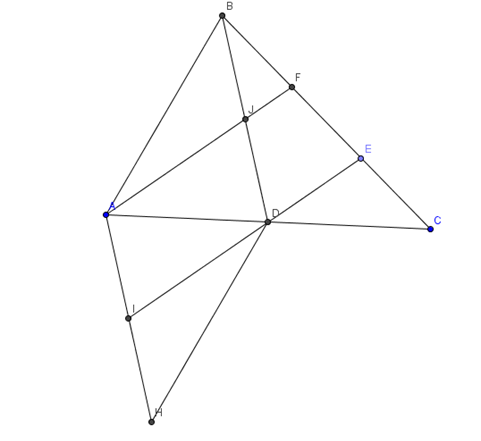
\includegraphics[scale=1]{imagenes/Geometria/1.png}
          \end{center}
          Llamemos $I$ a $ED\cap AH$, $F$ al segundo punto que triseca a $BC$ y $J$ a $AF\cap BD$. Luego se cumple que:\\
          $EC=EF$ y $AD=DC\Rightarrow AF\parallel ED$ ya que $AF$ sería paralela media del $\triangle AFC$.\\
          Apliquemos el teorema de las perpendiculares:
          $${BJ\over JD}={BF\over FE}$$
          $$\Rightarrow BJ=JD$$
          Pero se tiene que $AJDI$ y $ABDH$ son paralelogramos ya que $AJ\parallel ID$, $AB\parallel DH$ y $AH\parallel BD$.
          $BD=AH$ y $AI=JD$ por ser lados opuestos de un paralelogramo.\\
          Pero:
          $$BJ+JD=BD$$
          $$BJ=JD=AI=x$$
          $$\Rightarrow BD=2x$$
          $$AH=AI+HI$$
          Sustituyendo:
          $$2x=x+HI$$
          $$x=HI$$
          $\therefore$ Queda demostrado que $AI=HI$. Luego $ED$ biseca a $AH$ $\blacksquare$\\
    \item  Sea $ABCD$ un cuadrilátero cíclico. Sea $P$ la intersección de las rectas $BC$ y $AC$. La recta $AC$ corta a la circunferencia circunscrita del $\triangle BDP$ en $S$ y $T$, con $S$ entre $A$ y $C$. La recta $BD$ corta a la circunferencia circunscrita del $\triangle ACP$ en $U$ y $V$ , con $U$ entre $B$ y $D$. Demuestre que $PS = PT = PU = PV$ .
          Respuesta:
          \begin{center}
              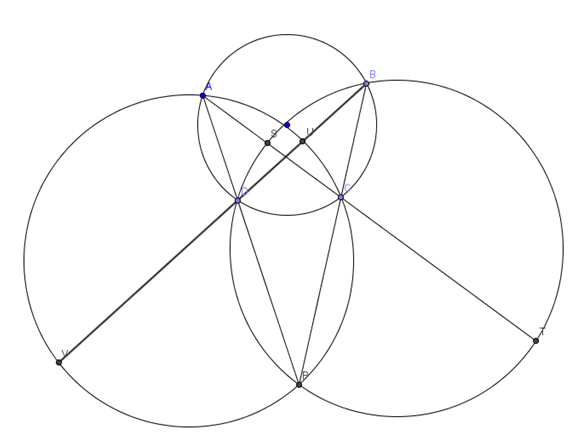
\includegraphics[scale=1]{imagenes/Geometria/2.png}
          \end{center}
          $$\angle DAC=\angle DBC=\alpha$$
          por estar inscritos sobre el mismo arco.\\
          Por ser ángulos exteriores a la circunferencia tenemos que:
          
          $$\angle VBP={\stackrel{\textstyle\frown}{\mathrm{VP}}-\stackrel{\textstyle\frown}{\mathrm{UC}}\over 2}=\alpha$$
          y
          $$\angle PAC={\stackrel{\textstyle\frown}{\mathrm{TP}}-\stackrel{\textstyle\frown}{\mathrm{SD}}\over 2}=\alpha$$
          Pero:
          $$\angle DBP={\stackrel{\textstyle\frown}{\mathrm{DP}}\over 2}=\alpha$$
          $$\angle CAP={\stackrel{\textstyle\frown}{\mathrm{CP}}\over 2}=\alpha$$
          $$\Rightarrow {\stackrel{\textstyle\frown}{\mathrm{DP}}\over 2}={\stackrel{\textstyle\frown}{\mathrm{TP}}-\stackrel{\textstyle\frown}{\mathrm{SD}}\over 2}$$
          $$\stackrel{\textstyle\frown}{\mathrm{DP}}+\stackrel{\textstyle\frown}{\mathrm{SD}}=\stackrel{\textstyle\frown}{\mathrm{TP}}$$
          $$\stackrel{\textstyle\frown}{\mathrm{SP}}=\stackrel{\textstyle\frown}{\mathrm{TP}}$$
          $$SP=TP$$
          y
          $$\Rightarrow {\stackrel{\textstyle\frown}{\mathrm{CP}}\over 2}={\stackrel{\textstyle\frown}{\mathrm{VP}}-\stackrel{\textstyle\frown}{\mathrm{UC}}\over 2}$$
          $$\stackrel{\textstyle\frown}{\mathrm{CP}}+\stackrel{\textstyle\frown}{\mathrm{UC}}=\stackrel{\textstyle\frown}{\mathrm{VP}}$$
          $$\stackrel{\textstyle\frown}{\mathrm{UP}}=\stackrel{\textstyle\frown}{\mathrm{VP}}$$
          $$UP=VP$$
          Digamos que $AC$ y $DB$ se intersecan en $E$. Luego apliquemos potencia del punto $E$ en las tres circunferencias:
          $$AE\cdot EC=DE\cdot EB$$
          $$AE\cdot EC=EV\cdot EU$$
          $$DE\cdot EB=SE\cdot ET$$
          $$\Rightarrow SE\cdot EL=EV\cdot EU$$
          Esto nos dice que $S$,$T$,$U$ y $V$ son concíclicos y como tenemos que $SP=TP$ y $UP=VP$, entonces tenemos que $P$ está en la mediatriz de $UV$ y de $ST$, luego $P$ es la intersección de las dos mediatrices y por tanto el centro de la circunferencia que pasa por $S$,$T$,$U$ y $V$.\\
          $\therefore$ $SP,VP,UP$ y $DP$ son radios y se cumple que $PS = PT = PU = PV$ $\blacksquare$\\
    \item Dado un $\triangle ABC$, sean $M$ y $N$ puntos variables de los lados $AB$ y $AC$, respectivamente, tales que ni $M$ ni $N$ coinciden con los vértices y, además, $AM \cdot MB = AN \cdot NC$. Pruebe que la mediatriz del segmento $MN$ pasa por un punto fijo. \\
          Respuesta:
          \begin{center}
              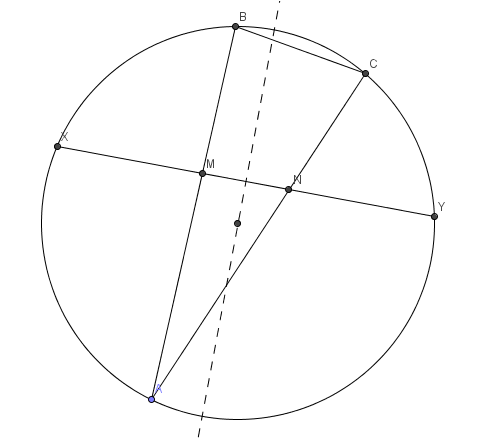
\includegraphics[scale=1]{imagenes/Geometria/3.png}
          \end{center}
          Tracemos el circuncírculo del $\triangle ABC$, luego tracemos la recta $MN$ que corta al circuncírculo en los puntos $X$ y $Y$.
          Ahora apliquemos potencia del punto $M$ y del punto $N$:
          $$XM\cdot MY=AM\cdot MB$$
          $$NY\cdot NX=AN\cdot NB$$
          Pero por datos tenemos que $AM\cdot MB = AN\cdot NC$ luego:
          $$\Rightarrow XM\cdot MY=NY\cdot NX$$
          $$XM(YN+MN)=YN(MN+XM)$$
          $$XM\cdot YN+MN\cdot XM=YN\cdot MN+YN\cdot XM$$
          $$MN\cdot XM=YN\cdot MN$$
          $$XM=YN$$
          $\therefore$ Como $XM=YN$, la mediatriz de $MN$ es la misma que la mediatriz de $XY$ y como esta última es una cuerda se cumple que la mediatriz pasa por el centro de la circunferencia, que es el circuncentro del $\triangle ABC$ $\blacksquare$\\
    \item Sea el $\triangle ABC$ tal que $\angle BAC = 90^0$ y $BA=CA$. Sea $M$ el punto medio de $BC$. Un punto $D\neq A$ es elegido en la semicircunferencia de diámetro $BC$ que contiene a $A$. La circunferencia circunscrita al $\triangle DAM$ intersecta a las rectas $DB$ y $DC$ en los puntos $E$ y $F$, respectivamente. Demostrar que $BE = CF$.\\
          Respuesta:
          \begin{center}
              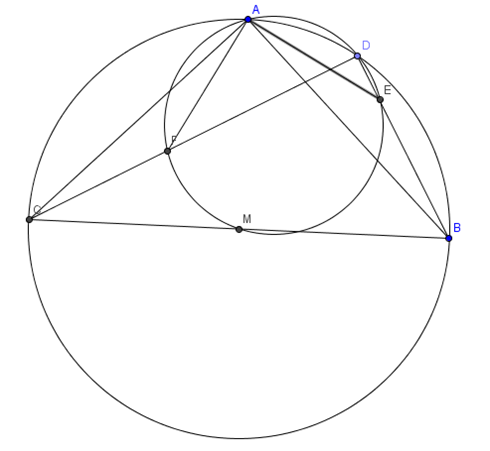
\includegraphics[scale=1]{imagenes/Geometria/4.png}
          \end{center}
          Por el teorema de tales se cumple que $A$ pertenece a la circunferencia con diámetro $BC$.
          Luego tenemos que:
          $$\angle ACD=\angle ABD$$
          $$\angle AFD=\angle AED$$
          por estar inscritos sobre el mismo arco.
          $$\angle AFD+\angle AFC={180}^0$$
          $$\angle AED+\angle AEB={180}^0$$
          por ser ángulos adyacentes.
          $$\Rightarrow\angle AFD+\angle AFC=\angle AED+\angle AEB$$
          $$\angle AFC=\angle AEB$$
          Por tanto se cumple que $\triangle AFC\sim\triangle AEB$ por tener dos ángulos iguales. Pero analicemos la proporción entre los elementos homólogos:
          $${AC\over AB}=1$$
          entonces como la razón de semejanza es 1 se cumple que $\triangle AFC=\triangle AEB$.\\
          $\therefore$ $CF=EB$ por ser elementos homólogos de los $\triangle AFC=\triangle AEB$ $\blacksquare$\\
    \item Sea un $\triangle ABC$ con baricentro en $G$, por $G$ se tras una recta $l$ que no contenga a ninguno de los vértices. Sean $P,Q$ y $R$ los pies de las alturas trazadas desde $C,A$ y $B$ a l respectivamente. Pruebe que $PC + RB = QA$. \\
          Respuesta:
          \begin{center}
              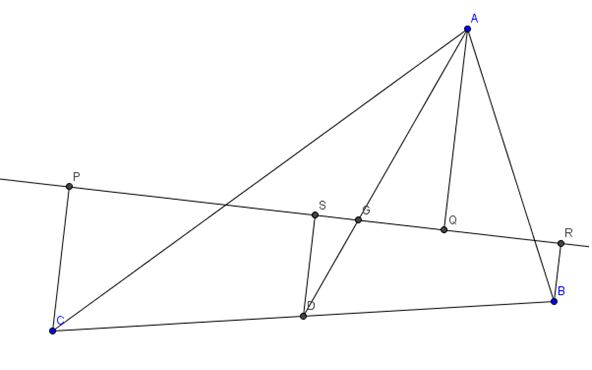
\includegraphics[scale=1]{imagenes/Geometria/5.png}
          \end{center}
          Digamos que $D$ es el punto medio de $BC$ y tracemos la mediana $AD$, luego ubiquemos un punto $S$ en $l$ tal que $DS$ sea perpendicular a $l$. Ahora tenemos que $RB\parallel SD\parallel PC$, por lo que se cumple que $RBCP$ es un trapecio de bases $RB$ y $PC$ y donde $SD$ es su paralela media:
          $$SD={RB+PC\over 2}$$
          $$\angle GSD=\angle GQA={90} ^0$$
          por ser $SD$ y $QA$ perpendiculares a $l$.
          $$\angle SGD=\angle QGA$$
          por estar opuestos por el vértice.\\
          
          Luego por ser $AD$ mediana y $G$ baricentro se cumple que:
          $${DG\over AG}={1\over 2}$$
          Estableciendo la proporcionalidad entre los elementos homólogos tenemos que:
          $${SD\over AQ}={SG\over GQ}={DG\over GA}={1\over 2}$$
          $${SD\over AQ}={1\over 2}$$
          $$2SD=AQ$$
          Sustituyendo:
          $$2\cdot{RB+PC\over 2}=AQ$$
          $$RB+PC=AQ$$
          $\therefore$ Se cumple que $RB+PC=AQ$ $\blacksquare$\\
    \item El punto $D$ está en lado $BC$ del $\triangle ABC$ tal que $\angle ABC = \angle DAC = 30^0$  y $ \angle ADB = 45^0$  .Pruebe que  $BD = DC$. \\
          Respuesta:
          \begin{center}
              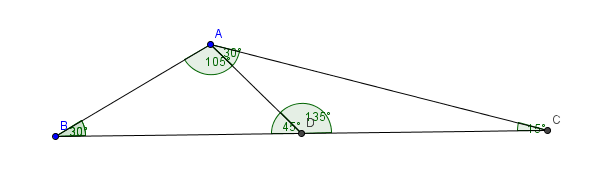
\includegraphics[scale=1]{imagenes/Geometria/6.png}
          \end{center}
          Apliquemos la ley de los senos:
          $$\frac{AD}{\sen{30^0}} =\frac{BD}{\sen{105^0} } $$
          $$\frac{AD}{\sen{15^0}} =\frac{DC}{\sen{30^0} }$$
          Dividiendo las dos ecuaciones:
          $$\frac{AD\cdot\sen{15^0}}{AD\cdot\sen{30^0}}=\frac{BD\cdot\sen{30^0}}{DC\cdot\sen{105^0} } $$
          $$\frac{\sen{105^0}\cdot\sen{15^0}}{\sen{30^0}\cdot\sen{30^0}}=\frac{BD}{DC} $$
          Luego para que $BD= DC$ se tiene que cumplir que:
          $$\frac{\sen{105^0}\cdot\sen{15^0}}{\sen{30^0}\cdot\sen{30^0}}=1 $$
          $$\sen{75^0}\cdot\sen{15^0}={1\over 4}$$
          $$\cos{15^0}\cdot\sen{15^0}={1\over 4}$$
          $$2\cdot\cos{15^0}\cdot\sen{15^0}={1\over 2}$$
          $$\sen{30^0}={1\over 2}$$
          Con lo que queda demostrada la identidad.\\
          $\therefore$ Se cumple que $BD= DC$ $\blacksquare$\\
    \item Sea un $\triangle ABC$ con $AC=AB$ y $\angle ABC = 40^0$. Sobre $BC$ se sitúa un punto $D$ tal que $AB=BD$, por $D$ se traza una paralela a $AB$ que interseca a $AC$ en $E$. Halle la amplitud del $\triangle EBD$.\\
          Respuesta:
          \begin{center}
              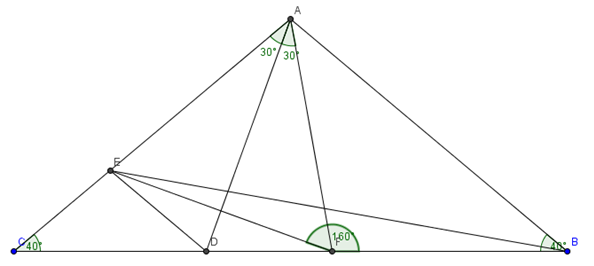
\includegraphics[scale=1]{imagenes/Geometria/7.png}
          \end{center}
          $\angle BDA=\angle DAB$  y $\angle ABC=\angle ACB=40^0$  por ser $\triangle ADB$ y $\triangle ABC$ isósceles de base $DA$ y $CA$ respectivamente.
          $$\angle ABC+\angle ACB=180^0-\angle CAB$$
          $$\angle CAB=100^0$$
          Luego como $\angle ABD=40^0\Rightarrow\angle BDA=\angle DAB=70^0$.
          $$\angle CAD+\angle DAB=\angle CAB$$
          $$\angle DAC=30^0$$
          $\angle DAB=\angle ADE$ por ser ángulos alternos entre paralelas.
          $$\Rightarrow\angle DAB=\angle ADE=\angle BDA=70^0$$
          Ahora ubiquemos en $CB$ un punto $F$ tal que $\angle DAF=\angle DAC=30^0$.
          $$\angle DAF+\angle FAB=\angle DAB$$
          $$\angle FAB=40^0$$
          Luego se cumple que el $\triangle FAB$ es isósceles de base $AB  \Rightarrow  AF=FB$.
          $$\angle FAB+\angle ABF=180^0-\angle AFB$$
          $$\angle AFB=100^0$$
          Entonces como $\angle ADE=\angle BDA$, $\angle DAF=\angle DAC$ y $DA$ lado común se cumple que $\triangle EAD=\triangle DAF$. \\
          $\Rightarrow  EA=AF$ por ser elementos homólogos.\\
          Entonces se cumple que $\triangle EAF$ es isósceles y un triángulo isósceles con un ángulo de $60^0$ es un triángulo equilátero.
          $$\Rightarrow  EA=AF=EF$$
          Ahora tenemos que:
          $$AF=FB \wedge AF=EF$$
          $$\Rightarrow  BF=EF$$
          Luego se cumple que el $\triangle FBE$ es isósceles de base $BF  \Rightarrow \angle FBE=\angle FEB$ .
          $$\angle AFB+\angle AFE=\angle EFB$$
          $$\angle FBE+\angle FEB+\angle EFB=180^0$$
          $$2x+160^0=180^0$$
          $$x=10^0$$
          $\therefore$ La amplitud del $\angle EBD$ es de $10^0$ $\blacksquare$\\
    \item En el $\triangle ABC$, rectángulo en $C$, sea $F$ el punto de intersección de la altura $CD$ y la bisectriz $AE$ y $G$, el punto de intersección de $ED$ y $BF$. Pruebe que el área del cuadrilátero $CEGF$ es igual al área del $\triangle BDG$.\\
          Respuesta:
          \begin{center}
              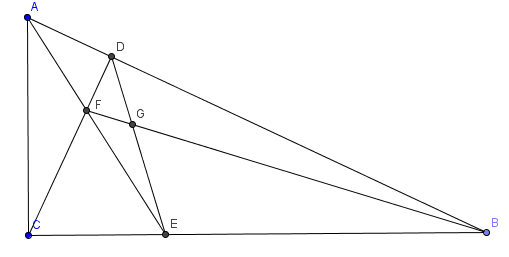
\includegraphics[scale=1]{imagenes/Geometria/8.png}
          \end{center}
          Denotemos $(ABC)$ como área del polígono $ABC$.
          Luego se cumple que:
          $${(FCB)\over(FDB)}={CF\over DF}$$
          porque estos dos triángulos tienen la misma base y la misma altura. Por la misma razón se cumple que:
          $${(CDE)\over(EDB)}={CE\over EB}$$
          Pero:
          $${CA\over AD}={CF\over DF}$$
          $${CD\over DB}={CE\over EB}$$
          por la propiedad de la bisectriz.\\
          Pero como los triángulos $\triangle ACD$ y $\triangle CDB$ son semejantes se tiene que:
          $${CA\over AD}={DB\over CD}$$
          por ser elementos homólogos.
          $$\Rightarrow{(FCB)\over(FDB)}={(EDB)\over(CDE)}$$
          $${(CFGE)+(EGB)\over(DGF)+(DGB)}={(DGB)+(EGB)\over(DFG)+(CFGE)}$$
          $${(CFGE)}^2+(CFGE)\cdot(DFG)+(EGB)\cdot(DFG)+(EGB)\cdot(CFGE)={(DGB)}^2+(DGB)\cdot(EGB)+(DGF)\cdot(EGB)+(DGF)\cdot(DGB)$$
          $$[(CFGE)-(DGB)][(CFGE)+(DGB)]+(DGF)[(CFGE)-(DGB)]+(EGB)[(CFGE)-(DGB)]=0$$
          $$[(CFGE)-(DGB)][(CFGE)+(DGB)+(DGF)+(EGB)]=0$$
          $$\Rightarrow(CFGE)-(DGB)=0 \vee (CFGE)+(DGB)+(DGF)+(EGB)=0$$
          la segunda igualdad es imposible porque una suma de áreas no puede dar cero, ya que las áreas son números positivos.
          $$\Rightarrow(CFGE)-(DGB)=0$$
          $\therefore$ Queda demostrado que el área del cuadrilátero $CEGF$ es igual al área del triángulo $BDG$ $\blacksquare$\\
    \item Sean $x,y$ y $z$ las amplitudes de los ángulos interiores de un triángulo tales que:
          $$\sen{x^2}+\sen{y^2}=\sen{z}$$
          Halle el valor de $z$. \\
          Respuesta:\\
          Dibujemos el triángulo correspondiente a dichos ángulos como se muestra en la figura, $a$,$b$ y $c$ son los segmentos opuestos a los ángulos $x$,$y$ y $z$ respectivamente. Luego tracemos el diámetro desde el vértice del ángulo $z$ y tracemos los segmentos $e$ y $d$ desde los vértices de los otros dos ángulos hasta el otro extremo del diámetro trazado anteriormente.
          Ahora apliquemos la ley de los senos:
          $${\sen {x}\over a}={\sen {y}\over b}={\sen {z}\over c}={1\over 2r}$$
          donde r es el radio de la circunferencia.
          Sustituyendo en la ecuación que teníamos inicialmente se tiene que:
          $${a^2\over 4r^2} +{b^2\over 4r^2} ={c\over 2r}$$
          $$a^2+b^2=2rc$$
          Apliquemos el teorema de Ptolomeo:
          $$be+da=2rc$$
          $$\Rightarrow be+da=a^2+b^2$$
          $$b(e-b)=a(a-d)$$
          \begin{center}
              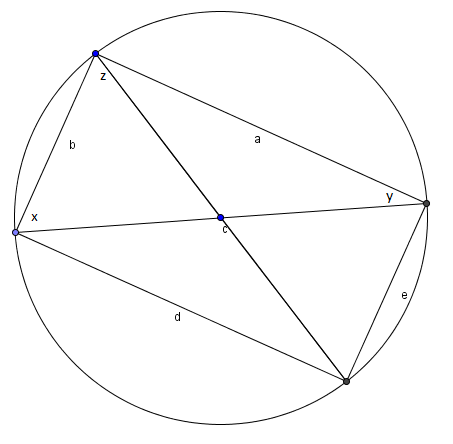
\includegraphics[scale=1]{imagenes/Geometria/9.png}
          \end{center}
          Pero por el teorema de Pitágoras tenemos que:
          $$a^2+e^2=4r^2$$
          y
          $$b^2+d^2=4r^2$$
          $$\Rightarrow a^2+e^2=b^2+d^2$$
          $$(a-d)(a+d)=(b-e)(b+e)$$
          Supongamos que $a\neq d$ y $b\neq e$, entonces se cumple que:
          $$\frac{(a-d)(a+d)}{a(a-d)}=\frac{(b-e)(b+e)}{b(e-b)} $$
          $$-b(a+d)=a(b+e)$$
          Este resultado es una contradicción ya que la ecuación nos dice hay variables negativas y las longitudes de los segmentos son números positivos. Luego tenemos que $a=d$ ó $b=e$ ó ambas igualdades son verdaderas.\\
          Para $a=d$ tenemos que:
          $$0=(b-e)(b+e)$$
          pero $b+e\neq 0$ porque las longitudes de los segmentos son números positivos:
          $$\Rightarrow b=e$$
          De manera análoga pasa lo mismo cuando analizamos el caso $b=e$.
          Entonces tenemos que $a=d$ y $b=e$, esto nos dice que el cuadrilátero formado por los lados $a$,$b$,$e$ y $d$ es un paralelogramo ya que tiene sus lados opuestos iguales y como además es cíclico entonces se cumple que es un rectángulo.\\
          $\therefore$ $z=90^0$ por ser ángulo interior de un rectángulo $\blacksquare$\\
    \item El $\triangle ABC$ está inscrito en una circunferencia $\Gamma$. Los puntos $X,Y,Z$ son los puntos medios de los arcos $\stackrel{\textstyle\frown}{\mathrm{BC}},\stackrel{\textstyle\frown}{\mathrm{CA}}$ y  $\stackrel{\textstyle\frown}{\mathrm{AB}}$ respectivamente en $\Gamma$ (los que no contienen el tercer vértice, en cada caso). Los puntos de intersección de los lados de los triángulos $\triangle ABC$ y $\triangle XYZ$ forman el hexágono $DEFGHK$. Prueba que las diagonales $DG,EH$ y $FK$ son concurrentes. \\
          Respuesta:
          \begin{center}
              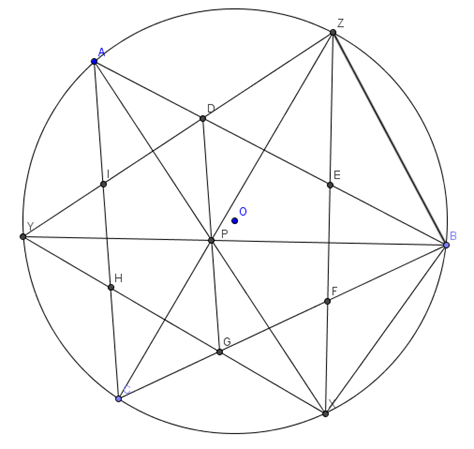
\includegraphics[scale=1]{imagenes/Geometria/10.png}
          \end{center}
          
          Pero por suma de ángulos interiores de un triángulo se tiene que:
          $$\angle XGB+\angle GBX+\angle BXG=180^0$$
          $$\angle XGB+\angle GBX=180^0-\angle BXG$$
          $$\angle ZDB+\angle ZBD+\angle BZD=180^0$$
          $$\angle ZDB+\angle ZBD=180^0-\angle BZD$$
          Sustituyendo:
          $$\angle GPX+\angle XPB=180^0-\angle BXG$$
          $$\angle DPZ+\angle ZPB=180^0-\angle BZD$$
          $$\Rightarrow\angle GPX+\angle XPB+\angle DPZ+\angle ZPB=360^0-\angle BXG-\angle BZD$$
          Pero como $YXBZ$ es cíclico se tiene que:
          $$\angle BXG+\angle BZD=180^0$$
          $$\Rightarrow\angle GPX+\angle XPB+\angle DPZ+\angle ZPB=360^0-180^0$$
          $$\Rightarrow\angle GPX+\angle XPB+\angle DPZ+\angle ZPB=180^0$$
          Luego se demuestra que $D$,$P$ y $G$ son colineales.\\
          Análogamente se demuestra que  $P\in HE$ y $P\in IF$.\\
          $\therefore$ Las diagonales $DG$,$EH$ y $FK$ concurren el incentro $P$ $\blacksquare$\\
    \item Sea $M$ el punto de intersección de las diagonales $AC$ y $BD$ del cuadrilátero convexo $ABCD$. Sea $K$ el punto de intersección de la prolongación del lado $AB$ (desde $A$) con la bisectriz del $\angle ACD$. Si $MA\cdot MC + MA\cdot CD =MB \cdot MD$ , demuestre que $\angle BKC = \angle CDB$. \\
          Respuesta:
          \begin{center}
              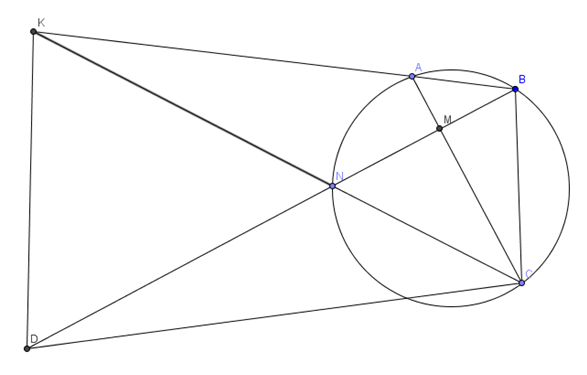
\includegraphics[scale=1]{imagenes/Geometria/11.png}
          \end{center}
          Digamos que $N=DB\cap KC$. Ahora apliquemos la propiedad de la bisectriz:
          $${NM\over MC}={ND\over DC}$$
          $$\Rightarrow{NM\over MC}={ND+MN\over DC+MC}$$
          $${NM\over MC}={MD\over DC+MC}$$
          Pero tenemos que:
          $$MA\cdot MC + MA\cdot CD = MB\cdot MD$$
          $$MA( MC+CD) = MB\cdot MD$$
          $$MC+CD={ MB\cdot MD\over MA}$$
          Sustituyendo:
          $${NM\over MC}=\frac{MD}{{MB\cdot MD\over MA}}$$
          $${NM\over MC}={MA\over MB}$$
          $$\Rightarrow NM\cdot MB=MA\cdot MC$$
          De aquí obtenemos que el cuadrilátero $NABC$ es cíclico ya que se cumple la potencia de un punto, por lo que tenemos que:
          $$\angle MCN=\angle MBA$$
          por estar inscritos sobre el mismo arco.\\
          Pero como $NC$ es bisectriz del $\angle MCD$ se cumple que:
          $$\angle MCN=\angle NCD$$
          $$\Rightarrow \angle MBA=\angle NCD$$
          Luego se cumple que cuadrilátero $DCBK$ es cíclico ya que los ángulos que están en posición de inscritos son iguales.\\
          $\therefore$ $\angle BKC=\angle CDB$ por estar inscritos sobre el mismo arco $\blacksquare$\\
    \item Sea $ABC$ un triángulo acutángulo y $D$ el pie de la altura desde $A$ sobre $BC$,$E$ y $F$ son los puntos medios de $BD$ y $DC$ respectivamente. $O$ y $Q$ son los circuncentros de los triángulos $\triangle ABF$ y $\triangle ACE$ respectivamente. $P$ es la intersección de $OE$ y $QF$, muestra que $PB=PC$. \\
          Respuesta:
          \begin{center}
              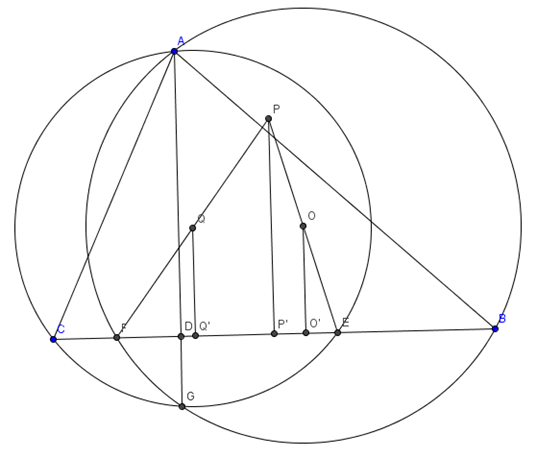
\includegraphics[scale=1]{imagenes/Geometria/12.png}
          \end{center}
          Digamos que $AD$ corta al circuncírculo del $\triangle ABF$ en $G$ y al circuncírculo del $\triangle ACE$ en $G^{'}$, luego por potencia de un punto se cumple que:
          $$AD\cdot DG=FD\cdot DB$$
          $$AD\cdot DG=FD\cdot 2DE$$
          y
          $$AD\cdot DG^{'}=CD\cdot DE$$
          $$AD\cdot DG^{'}=2FD\cdot DE$$
          $$\Rightarrow AD\cdot DG^{'}=AD\cdot DG$$
          $$DG^{'}=DG$$
          $$G^{'}=G$$
          Luego tenemos que AD es el eje radical de los dos circuncírculos:
          $$\Rightarrow AD\perp OQ$$
          $$\Rightarrow OQ\parallel BC$$
          por ser ángulos correspondientes.\\
          Ubiquemos los puntos $P^{'}$,$O^{'}$ y $Q^{'}$ tal que los segmentos $PP^{'}$, $OO^{'}$ y  $QQ^{'}$ sean perpendiculares a $AD$. Ahora apliquemos el teorema de las perpendiculares:
          $${FQ\over QP}={EO\over OP}$$
          $${FQ\over QP}={FQ^{'}\over Q^{'} P^{'} }$$
          $${EO\over OP}={EO^{'}\over O^{'} P^{'} }$$
          $$\Rightarrow{FQ^{'}\over Q^{'} P^{'} }={EO^{'}\over O^{'} P^{'} }$$
          Digamos que:
          $$CF=FD=a$$
          $$DQ^{'}=c$$
          $$Q^{'} P^{'}=d$$
          $$P^{'} O^{'}=e$$
          $$O^{'} E=f$$
          $$EB=c+d+e+f$$
          Sustituyendo:
          $${a+c\over d}={f\over e} $$
          $${f\over e}={a+c+f\over e+d}\;  (1)$$
          Pero como $O$ y $Q$ son los circuncentros $\triangle ABF$ y $\triangle ACE$ respectivamente y $OO^{'}$ y  $QQ^{'}$ son perpendiculares a $AD$ se tiene que:
          $$CQ^{'}=Q^{'} E$$
          $$2a+c=d+e+f\; (2)$$
          y
          $$FO^{'}=O^{'} B$$
          $$c+d+e+2f=a+c+d+e$$
          $$2f=a\; (3)$$
          Sustituyendo (3) en (2):
          $$4f+c=d+e+f $$
          $$3f+c=d+e\; (4)$$
          Sustituyendo (3) y (4) en (1):
          $${f\over e}={2f+c+f\over 3f+c}$$
          $$\Rightarrow f=e\Rightarrow a+c=d$$
          Ahora tenemos que:
          $$a=2f$$
          $$a=e+f$$
          $$2a=2e+2f$$
          $$2a+c+d=e+f+c+d+e+f$$
          $$\Rightarrow CP^{'}=P^{'} B$$
          $\therefore$ Como $P^{'}$ es la base de la perpendicular trazada desde $P$ a $BC$ y $CP^{'}=P^{'} B$ se cumple que el $\triangle PBC$ es isósceles de base $BC$, luego  $PB = PC$ $\blacksquare$\\
    \item Sea $ABCD$ un trapecio con $AB > CD$, cuyas bases son $AB$ y $CD$, sobre estas se sitúan los puntos $G$ y $F$ respectivamente tal que:
          $$\frac{CF}{FD}=\frac{AG}{GB}$$
          Sea $X$ y $Y$ los puntos de intersección de los segmentos $CG$ y $AF$, $GD$ y $FB$ respectivamente. Demuestre que $XY \parallel AB$. \\
          Respuesta:
          \begin{center}
              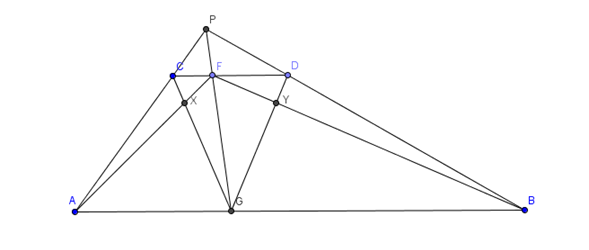
\includegraphics[scale=1]{imagenes/Geometria/13.png}
          \end{center}
          Llamemos $P$ a la intersección de $AC$ y $DB$. Luego tracemos $PG$ y digamos que corta a $CD$ en $F^{'}$ y apliquemos el teorema de las transversales:
          $${CF^{'}\over F^{'} D}={AG\over GB}$$
          $$\Rightarrow {CF\over FD}={CF^{'}\over F^{'} D}$$
          $${CD-FD\over FD}={CD-F^{'} D\over F^{'} D}$$
          $$CD\cdot F^{'} D-FD\cdot F^{'} D=CD\cdot FD-FD\cdot F^{'} D$$
          $$CD\cdot F^{'} D=CD\cdot FD$$
          $$F^{'} D=FD$$
          $$\Rightarrow F^{'}=F$$
          Hemos demostrado que $P$, $F$ y $G$ son colineales, ahora apliquemos el teorema de Menelao:
          $${PD\over DB}\cdot {BY\over YF}\cdot {FG\over GP}=1$$
          $${PC\over CA}\cdot {CX\over XF}\cdot {FG\over GP}=1$$
          Dividiendo las dos ecuaciones se tiene que:
          $${PD\over DB}\cdot {BY\over YF}\cdot {FG\over GP}\cdot {CA\over PC}\cdot {XF\over CX}\cdot {GP\over FG}=1$$
          $${PD\over DB}\cdot{BY\over YF}\cdot {CA\over PC}\cdot {XF\over CX}=1$$
          Pero por el teorema de las transversales se tiene que:
          $${PD\over DB}={PC\over CA}$$
          $${PD\over DB}\cdot{CA\over PC}=1$$
          Sustituyendo:
          $${BY\over YF}\cdot{XF\over CX}=1$$
          $${BY\over YF}={CX\over XF}$$
          $\therefore$ Por el recíproco del teorema de las transversales se cumple que $XY\parallel AB$ $\blacksquare$\\
    \item En el paralelogramo $ABCD$, la recta paralela a $BC$ corta a $AB$ y $CD$, respectivamente, en los puntos $E$ y $F$, la recta paralela a $AB$ corta a $BC$ y $DA$, respectivamente, en los puntos $G$ y $H$. Demostrar que las rectas $EH,GF$ y $BD$ se intersecan en un punto o son paralelas. \\
          Respuesta:
          \begin{center}
              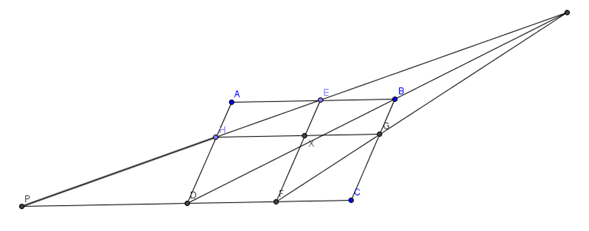
\includegraphics[scale=1]{imagenes/Geometria/14.png}
          \end{center}
          El caso en que las rectas son paralelas se cumple cuando $E$ y $G$ son los puntos medios de los segmentos $AB$ y $BC$ respectivamente, ya que $EH$ y $GF$ son paralelas medias de los $\triangle ABD$ y $\triangle BCD$ por tanto $HE\parallel BD\parallel GF$.\\
          Ahora demostremos la concurrencia. Digamos que $Q=HE\cap FQ$, $P=HE\cap DC$ y$ M=EB\cap QG$.\\
          Entonces apliquemos el teorema de Menelao tomando como puntos meneláicos a $E$,$X$ y $F$:
          $${HE\over EO}\cdot{OF\over FG}\cdot{GX\over XH}=1$$
          Apliquemos el teorema de Menelao tomando como puntos meneláicos a $G$,$X$ y $H$:
          $${FG\over GO}\cdot{OH\over HE}\cdot{EX\over FX}=1$$
          Igualando las dos expresiones:
          $${HE\over EO}\cdot{OF\over FG}\cdot{GX\over XH}={GO\over FG}\cdot{HE\over OH}\cdot{FX\over EX}$$
          $${OF\over EO}\cdot{GX\over XH}={GO\over OH}\cdot{FX\over XE}$$
          Pero por el teorema de las transversales tenemos que:
          $${FX\over XE}={PH\over HE}$$
          $${HP\over HE}={PD\over DF}$$
          $$\Rightarrow{HP\over HE}={PD\over DF}={FX\over XE}$$
          y
          $${OM\over EO}={GO\over OH}$$
          Sustituyendo:
          $${OF\over EO}\cdot{GX\over XH}={OM\over EO}\cdot{PD\over DF}$$
          Luego por ser lados opuestos de un paralelogramo tenemos que:
          $$GX=EB$$
          y
          $$HX=DF$$
          Sustituyendo:
          $${OF\over EO}\cdot{EB\over DF}={OM\over EO}\cdot{PD\over DF}$$
          $${OF\over OM}={PD\over EB}$$
          Ahora por el teorema de las transversales tenemos que:
          $${OF\over OM}={PF\over EM}$$
          $$\Rightarrow{OF\over OM}=\frac{PF-PD}{EM-EB}={DF\over BM}$$
          $$\Rightarrow{DF\over BM}={PD\over EB}$$
          $${EB\over BM}={PD\over DF}$$
          Supongamos que $R=BQ\cap DC$, entonces por transversales se cumple que:
          $${EB\over BM}={PR\over RF}$$
          $$\Rightarrow{PD\over DF}={PR\over RF}$$
          $${PF-DF\over DF}={PF-RF\over RF}$$
          $${PF\over DF}-1={PF\over RF}-1$$
          $$\Rightarrow DF=RF\Rightarrow PD=PR$$
          $$\Rightarrow R=D$$
          $\therefore$ Se cumple que $Q$, $B$ y $D$ son colineales y entonces tenemos que $EH$,$GF$ y $BD$ se intersecan en $Q$ $\blacksquare$\\
    \item Se inscribe una circunferencia en el interior de un cuadrilátero $ABCD$. Sea $E$ y $F$ los puntos de intersección de las rectas $AD$ y $BC$, y $AB$ y $DC$ respectivamente. Los puntos de tangencia de la circunferencia con los segmentos $AB,DC,AD$ y $BC$ son $P,Q,R$ y $S$ respectivamente. Demuestre que si los puntos $E,P$ y $Q$ están alineados entonces los puntos $F,R$ y $S$ son colineales.\\
          Respuesta:
          \begin{center}
              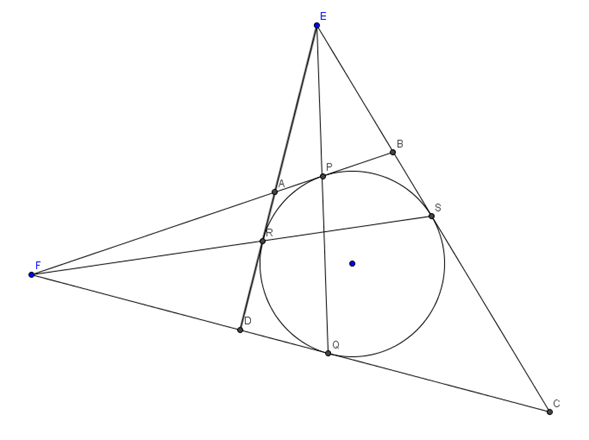
\includegraphics[scale=1]{imagenes/Geometria/15.png}
          \end{center}
          Como las tangentes trazadas desde un punto exterior hacia la circunferencia son iguales se cumple que:
          $$AP=AR=a$$
          $$RD=DQ=b$$
          $$QC=CS=c$$
          $$SB=PB=d$$
          Apliquemos la ley de los senos:
          $${\sen {\angle EAP}\over EP}={\sen {\angle AEP}\over a}$$
          $${\sen {\angle EBP}\over EP}={\sen {\angle PEB}\over d}$$
          $$\Rightarrow\frac{\sen {\angle EAP}}{\sen {\angle EBP}}=\frac{\sen {\angle AEP}\cdot d}{\sen {\angle PEB}\cdot a}\;(1)$$
          Apliquemos la ley de los senos:
          $${\sen {\angle EDQ}\over EQ}={\sen {\angle DEQ}\over b}$$
          $${\sen {\angle ECQ}\over EQ}={\sen {\angle QEC}\over c}$$
          $$\Rightarrow{\sen {\angle EDQ}\over\sen {\angle ECQ}}={\sen {\angle DEQ}\cdot c\over\sen {\angle QEC}\cdot b}\;  (2)$$
          Dividiendo las expresiones (1) y (2) tenemos que:
          $$\frac{\sen {\angle EAP}\cdot\sen {\angle ECQ}}{\sen {\angle EBP}\cdot\sen {\angle EDQ}}={db\over ac}  $$
          $$\frac{\sen {\angle EAP}\cdot\sen {\angle ECQ}\cdot ac}{\sen {\angle EBP}\cdot\sen {\angle EDQ}\cdot bd}=1$$
          Pero:
          $$\sen {\angle EAP}=\sen {\angle FAR}$$
          por ser ángulos opuestos por el vértice y además:
          $$sen {\angle EBP}=sen {\angle FBS}$$
          $$sen {\angle EDQ}=sen {\angle FDR}$$
          Por ser ángulos adyacentes.\\
          Sustituyendo:
          $$\frac{\sen {\angle FAR}\cdot\sen {\angle ECQ}\cdot ad)}{\sen {\angle FDR}\cdot\sen {\angle FBS}\cdot bd}=1\; (3)$$
          Apliquemos la ley de los senos:
          $${\sen {\angle FAR}\over FR}={\sen {\angle AFR}\over a}$$
          $${\sen {\angle FDR}\over FR}={\sen {\angle RFD}\over b}$$
          $$\Rightarrow\frac{\sen {\angle FAR}}{\sen {\angle FDR}}=\frac{\sen {\angle AFR}\cdot b}{\sen {\angle RFD}\cdot a}\;(4)$$
          Apliquemos la ley de los senos:
          $${\sen {\angle FBS}\over FS}={\sen {\angle BFS}\over d}$$
          $${\sen {\angle FCS}\over FS}={\sen {\angle SFC}\over c}$$
          $$\Rightarrow\frac{\sen {\angle FBS}}{\sen {\angle FCS}}=\frac{\sen {\angle BFS}\cdot c}{\sen {\angle SFC}\cdot d}\;(5)$$
          Dividiendo las expresiones (4) y (5) tenemos que
          $$\frac{\sen {\angle FAR}\cdot\sen {\angle FCS}}{\sen {\angle FDR}\cdot\sen {\angle FBS}}=\frac{\sen {\angle AFR}\cdot\sen {\angle SFC}\cdot bd}{\sen {\angle RFD}\cdot\sen {\angle BFS}\cdot ac}$$
          $$\frac{\sen {\angle FAR}\cdot\sen {\angle FCS}\cdot ad}{\sen {\angle FDR}\cdot\sen {\angle FBS}\cdot bd}=\frac{\sen {\angle AFR}\cdot\sen {\angle SFC}}{\sen {\angle RFD}\cdot\sen {\angle BFS}}$$
          Sustituyendo por (3):
          $$1=\frac{\sen {\angle AFR}\cdot\sen {\angle SFC}}{\sen {\angle RFD}\cdot\sen {\angle BFS}}$$
          $$\frac{\sen {\angle BFS}}{\sen {\angle SFC}}=\frac{\sen {\angle AFR}}{
                  sen {\angle RFD}}$$
          $$\frac{\sen {\angle BFC-\angle SFC}}{\sen {\angle SFC}}=\frac{\sen {\angle AFD-\angle RDF}}{\sen {\angle RFD}}$$
          $$\frac{\sen{\angle BFC}\cdot\cos{\angle SFC}-cos{\angle BFC}\cdot\sen {\angle SFC}}{\sen{\angle SFC}}=\frac{\sen{\angle AFD}\cdot\cos{\angle RFD}-\cos{\angle AFD}\cdot\sen{\angle RDF}}{\sen{\angle RFD}}$$
          $$\sen {\angle BFC}\cdot\cot{\angle SFC}-\cos{\angle BFC}=\sen {\angle AFD}\cdot\cot{\angle RDF}-\cos{\angle AFD}$$
          $$\sen {\angle BFC}\cdot\cot{\angle SFC}=\sen {\angle AFD}\cdot\cot{\angle RDF}$$
          $$\cot{\angle SFC}=\cot{\angle RDF}$$
          $$\Rightarrow\angle SFC=\angle RDF$$
          ya que son ángulos del primer cuadrante. Luego por resta de ángulos consecutivos llegamos a:
          $$\angle AFR=\angle BFS$$
          $\therefore$ Como $\angle SFC=\angle RDF$ y $\angle AFR=\angle BFS$, tenemos que $R$ pertenece a la recta $BS$, por lo que $F$,$R$ y $S$ son colineales  $\blacksquare$\\
    \item En el $\triangle ABC$, $D ,E$ y $F$ son los pies de las alturas sobres los lados $BC,AC$ y $AB$ respectivamente. Sean $P,Q,R$ y $S$ los pies de las perpendiculares trazadas desde $D$ a $BA, BE, CF$ y $AC$ respectivamente. Probar que $P, Q, R$ y $S$ están sobre una misma recta.\\
          Respuesta:
          \begin{center}
              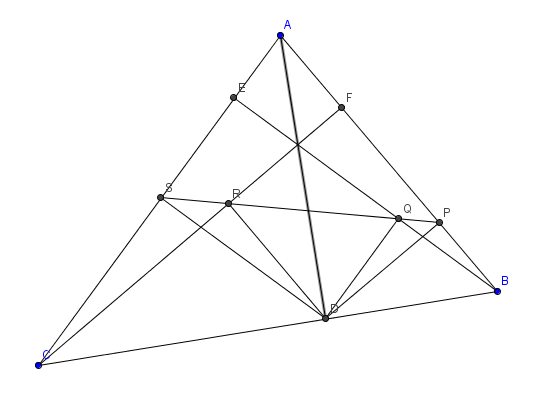
\includegraphics[scale=1]{imagenes/Geometria/16.png}
          \end{center}
          Tenemos que:
          $$\angle CSD=\angle CRD=90^0$$
          $$\angle DQB=\angle DPB=90^0$$
          $$\angle DSA+\angle DPA=90^0+90^0=180^0$$
          $$\angle AEB=\angle ADB=90^0$$
          $$\angle AFC=\angle ADC=90^ 0$$
          Por tanto se cumple que los cuadriláteros $CSRD$, $DQPB$, $APDS$, $AEDB$ y $AFDC$ son cíclicos:
          $$\angle PSD=\angle PAD$$
          $$\angle SPD=\angle SAD$$
          $$\angle RSD=\angle RCD$$
          $$\angle QPD=\angle QBD$$
          $$\angle EAD=\angle EBD$$
          $$\angle FAD=\angle FCD$$
          por sestar inscrito sobre el mismo arco.
          $$\Rightarrow\angle FCD=\angle DAF=\angle PSD=\angle RSD$$
          y
          $$\Rightarrow\angle EBD=\angle EAD=\angle SPD=\angle QPD$$
          $\therefore$ Como $\angle PSD=\angle RSD$ y $\angle SPD=\angle QPD$ se cumple que $R$ y $Q$ pertenecen a al segmento $SP$, entonces $S$,$R$,$Q$ y $P$ están alineados $\blacksquare$\\
    \item Sea $DA$ la altura de un triángulo acutángulo $\triangle ABC$, con respecto al vértice $A$. Sobre la recta $AD$ se toman puntos distintos $E$ y $F$ tal quede $DE=DF$, con e en el interior del $\triangle ABC$. El circuncírculo del $\triangle BEF$ corta a los segmentos $BC$ y $AB$ en los puntos $K$ y $M$ respectivamente. El circuncírculo del $\triangle CEF$ corta a los segmentos $BC$ y $AC$ en los puntos $L$ y $N$ respectivamente. Demuestre que $AD, KM$ y $LN$ concurren.\\
          Respuesta:
          \begin{center}
              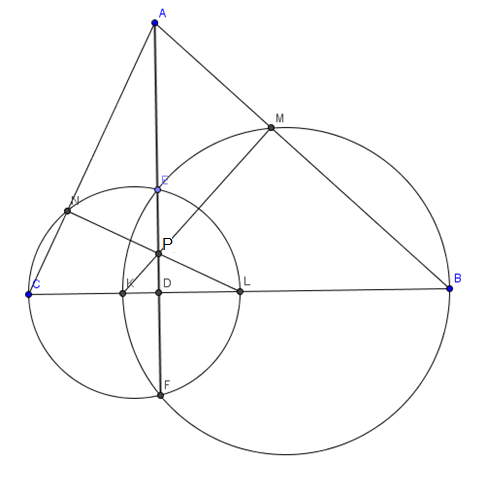
\includegraphics[scale=1]{imagenes/Geometria/17.png}
          \end{center}
          Digamos que:
          $$P=NL\cap KM$$
          $$\angle NLC=x$$
          $$\angle MKB=y$$
          Como $ED=DF$ y $CD$ y $DB$ son perpendiculares a $EF$ entonces tenemos por igualdad de triángulos que los  $\triangle CEF$ y $\triangle EBF$ son isósceles de base $EF$. Pero también se cumple que $CB$ es la mediatriz del segmento $EF$, luego tenemos que los circuncenrtros de los dos triángulos están sobre $BC$, entonces $CL$ y $KM$ son diámetros:
          $$\angle CNL=90^0$$
          $$\angle KMB=90^0$$
          Por ser ángulos complementarios tenemos que:
          $$\angle NLC+\angle NCL=90^0$$
          $$\angle NCL=90^0-x$$
          y
          $$\angle MKB+\angle MBK=90^0$$
          $$\angle MBK=90^0-y$$
          Apliquemos potencia de un punto al punto $A$:
          $$AN\cdot AC=AE\cdot AF$$
          $$AM\cdot AB=AE\cdot AF$$
          $$\Rightarrow AN\cdot AC=AM\cdot AB$$
          Luego se cumple que el cuadrilátero $CNMB$ es cíclico:
          $$\angle CNM+\angle MBC=180^0$$
          $$\angle MNL+90^0+90^0-y=180^0$$
          $$\angle MNL=y$$
          y
          $$\angle NMB+\angle NCB=180^0$$
          $$\angle NMK+90^0+90^0-x=180^0$$
          $$\angle NMK=x$$
          Por ser ángulos complementarios tenemos que:
          $$\angle DCA+\angle CAD=90^0$$
          $$\angle CAD=x$$
          y
          $$\angle BAD+\angle ABD=90^0$$
          $$\angle BAD=y$$
          Ahora nótese que:
          $$\angle PNA+\angle PMA=90^0+90^0=180^0$$
          Luego el cuadrilátero $PNAM$ es cíclico:
          $$\angle NMP=\angle NAP=x$$
          $$\angle MNP=\angle PAM=y$$
          $$\Rightarrow\angle NAÑ=\angle NAD=x$$
          $$\Rightarrow\angle DAM=\angle ÑAM=y$$
          $\therefore$ Se cumple que $P$ está sobre la recta $AD$, luego $AD$,$NL$ y $KM$ concurren $\blacksquare$\\
    \item Sea $P$ un punto interior del $\triangle ABC$. La circunferencia inscrita en el $\triangle ABC$ toca a los lados $BC,CA$ y $AB$ en los puntos $D,I$ y $F$ respectivamente $L,M$ y $N$ son Ios puntos de intersección de las recta $AP,BP$ y $CP$ con los lados $EF,FD$ y $DE$ del $\triangle DEF$. Muestre que las rectas $DL,EM$ y $FN$ son concurrentes en un punto.\\
          Se cumple que:
          $$\angle EMN=\angle CEN$$
          $$\angle NLD=\angle NCD$$
          por ser inscrito y seminscrito sobre el mismo arco.\\
          Apliquemos la ley de los senos:
          $${\sen {\angle ECN}\over NE}={\sen {\angle CEN}\over NC} \; (1)$$
          $${\sen {\angle NDC}\over NC}={\sen {\angle NCD}\over ND} \; (2)$$
          $${NE\over 2r}=\sen {\angle NME}=\sen {\angle CEN}\; (3)$$
          $${ND\over 2r}=\sen {\angle NLD}=\sen {\angle NDC}\; (4)$$
          Multiplicando (1) y (3) se tiene que:
          $${\sen {\angle ECN}\over NE}\cdot{ NE\over 2r}={\sen {\angle CEN}\cdot \sen {\angle NME}\over NC}  $$
          $$NC={\sen^2  {\angle NME}\over\sen {\angle ECN}}\cdot 2r$$
          Multiplicando (2) y (4) se tiene que:
          $${\sen {\angle NCD}\over ND}\cdot{ND\over 2r}={\sen {\angle NDC}\cdot\sen {\angle NLD}\over NC}$$
          $$NC={\sen^2  {\angle NLD}\over\sen {\angle NCD}}\cdot 2r$$
          $$\Rightarrow{\sen^2  {\angle NME}\over\sen {\angle ECN}}={\sen^2  {\angle NLD}\over\sen {\angle NCD}}$$
          $${\sen^2  {\angle NME}\over\sen^2  {\angle NLD}}={\sen {\angle ECN}\over\sen {\angle NCD}}$$
          De manera análoga se cumple que:
          $${\sen^2  {\angle DLM}\over\sen^2  {\angle FNM}}={\sen {\angle DBM}\over\sen {\angle MBF}}$$
          y
          $${\sen^2  {\angle LNF}\over\sen^2  {\angle EML}}={\sen {\angle LAF}\over\sen {\angle LAE}}$$
          Multiplicando miembro a miembro se tiene que:
          $${\sen^2  {\angle NME}\over\sen^2  {\angle NLD}}\cdot{\sen^2  {\angle DLM}\over\sen^2  {\angle FNM}}\cdot{\sen^2  {\angle LNF}\over\sen^2  {\angle EML}}={\sen {\angle ECN}\over\sen {\angle NCD}}\cdot{\sen {\angle DBM}\over\sen {\angle MBF}}\cdot{\sen {\angle LAF}\over\sen {\angle LAE}}$$
          Pero por el teorema de Ceva tenmos que:
          $${\sen {\angle ECN}\over\sen {\angle NCD}}\cdot{\sen {\angle DBM}\over\sen {\angle MBF}}\cdot{\sen {\angle LAF}\over\sen {\angle LAE}}=1$$
          Sustituyendo:
          $${\sen^2  {\angle NME}\over\sen^2  {\angle NLD}}\cdot{\sen^2  {\angle DLM}\over\sen^2  {\angle FNM}}\cdot{\sen^2  {\angle LNF}\over\sen^2  {\angle EML}}=1$$
          $${\sen  {\angle NME}\over\sen  {\angle NLD}}\cdot{\sen  {\angle DLM}\over\sen  {\angle FNM}}\cdot{\sen  {\angle LNF}\over\sen  {\angle EML}}=1$$
          Ya que los ángulos no son ni del tercer ni del cuarto cuadrante.\\
          $\therefore$ Por el teorema de Ceva se cumple que las rectas $DL$,$EM$ y $FN$ son concurrentes en un punto $\blacksquare$\\
    \item Sea $ABC$ un triángulo y $\Gamma$ su circuncírculo. Sean $D$ el pie de la altura trazada desde $A$ al lado $BC, M$ y $N$ los puntos medios de los segmentos de $AB$ y $AC$ respectivamente, y $Q$ el punto en $\Gamma$ diametralmente opuesto a $A$. Sea $E$ el punto medio de $DQ$. Muestre que las perpendiculares a $EM$ y $EN$ que pasan por $M$ y $N$ respectivamente, se cortan en $AD$.  \\
          Respuesta:
          \begin{center}
              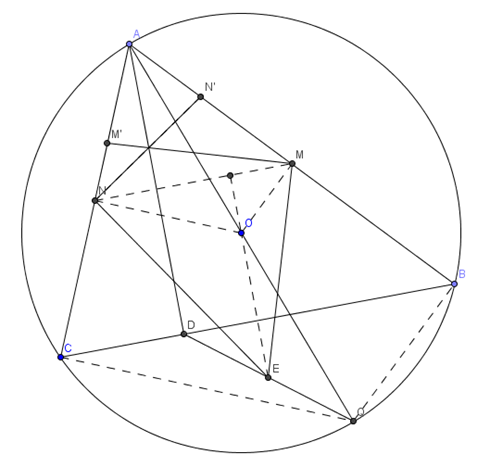
\includegraphics[scale=1]{imagenes/Geometria/19.png}
          \end{center}
          Tracemos los segmentos $MN,CQ,QB,EO,ON$ y $OM$. Luego por Tales:
          $$\angle QCA=90^0$$
          $$\angle QBA=90^0$$
          Ahora como $N,M,O$ y $E$ son puntos medios de los segmentos $CA,AB,QA$ y $DQ$ respectivamente se cumple que $MN,ON,OM$ y $OE$ son paralelas medias de los triángulos $\triangle ABC,\triangle AQC,\triangle AQB$ y $\triangle AQD$ respectivamente. Luego por ángulos correspondientes entre paralelas se tiene que:
          $$\angle ANO=\angle QCA=90^0$$
          $$\angle AMO=\angle QBA=90^0$$
          Además $OE\perp CB\Rightarrow OE\perp MN$.\\
          Llamemos $N^{'}$ a la intersección de la perpendicular a $NE$ por $N$ con $AB$ y  $M^{'}$ a la intersección de la perpendicular a $ME$ por $M$ con $AC$.
          $$\angle N^{'} NE=\angle ANO=90^0$$
          $$\angle M^{'} ME=\angle AMO=90^0$$
          $$\Rightarrow\angle N^{'}NE=\angle ANO$$
          $$\angle N^{'} NO+\angle ONE=\angle ANN^{'}+\angle N^{'} NO$$
          $$\angle ONE=\angle ANN^{'}=x$$
          $$\Rightarrow\angle M^{'} ME=\angle AMO$$
          $$\angle M^{'} MO+\angle OME=\angle AMM^{'}+\angle M^{'} MO$$
          $$\angle OME=\angle AMM^{'}=y$$
          Digamos que:
          $$\angle CAD=\alpha$$
          $$\angle DAB=\beta$$
          Por suma de ángulos interiores de un triángulo se tiene que:
          $$\angle CAD+\angle DCA+\angle ADC=180^0$$
          $$\angle DCA=90^0-\alpha$$
          $$\angle DAB+\angle ABD+\angle BDA=180^0$$
          $$\angle DBA=90^0-\beta$$
          Por ser ángulos correspondientes se cumple que:
          $$\angle ANM=\angle DCA=90^0-\alpha$$
          $$\angle AMN=\angle DBA=90^0-\beta$$
          Por ser ángulos adyacentes se cumple que:
          $$\angle ANM+\angle MNC=180^0$$
          $$\angle MNC=90^0+\alpha$$
          y
          $$\angle AMN+\angle NMB=180^0$$
          $$\angle NMB=90^0+ \beta$$
          Por suma de ángulos se tiene que:
          $$\angle MN0+\angle ONC=90^0+\alpha$$
          $$\angle MN0=\alpha$$
          y
          $$\angle NMO+\angle OMB=90^0+ \beta$$
          $$\angle NMO=\beta$$
          $$\angle ANM=\angle ANN^{'}+\angle N^{'}NM$$
          $$90^0-\alpha-x=\angle N^{'}NM$$
          y
          $$\angle AMN=\angle AMM^{'}+\angle M^{'}MN$$
          $$90^0-\beta-y=\angle M^{'}MN$$
          Por ser ángulos complementarios se tiene que:
          $$\angle MNE+\angle OEN=90^0$$
          $$\angle OEN=90^0-\alpha-x$$
          y
          $$\angle NME+\angle OEM=90^0$$
          $$\angle OEM=90^0-\beta-y$$
          Ahora como $OE,OM$ y $ON$ concurren, apliquemos el teorema de Ceva:
          $${\sen {\angle MNO}\over\sen {\angle ONE}}\cdot{\sen {\angle OEN}\over\sen {\angle OEM}}\cdot{\sen {\angle EMO}\over\sen {\angle OMN}}=1$$
          $${\sen \alpha\over\sen x}\cdot{\sen {90^0-\alpha-x}\over\sen {90^0-\beta-y}}\cdot{sen y\over\sen \beta}=1$$
          Pero sustituyendo:
          $${\sen \alpha\over\sen \beta}\cdot{\sen y\over\sen {90^0-\beta-y}}\cdot{\sen {90^0-\alpha-x}\over\sen x}=1$$
          $${\sen {\angle NAD}\over\sen {\angle DAM}}\cdot{\sen {\angle AMM^{'}}\over\sen {\angle M^{'} MN}}\cdot{\sen {\angle MNN^{'}}\over\sen {\angle N^{'} NA}}=1$$
          $\therefore$ Se cumple por el teorema de Ceva que $MM^{'},NN^{'}$ y $AD$ concurren, entonces se cumple que las perpendiculares a $EM$ y $EN$ que pasan por $M$ y $N$ respectivamente, se cortan en $AD$ $\blacksquare$\\
    \item Sea un $\triangle ABC$, sobre los lados $AB$ y $AC$ se inscriben dos triángulos isorectángulos $ABD$ y $ACE$ respectivamente, de tal manera que $D$ y $E$ son puntos en exterior del $\triangle ABC$. Sea $F$ el punto medio de $BC$, pruebe que el $\triangle DEF$ es isorectángulo.\\
          Respuesta:
          \begin{center}
              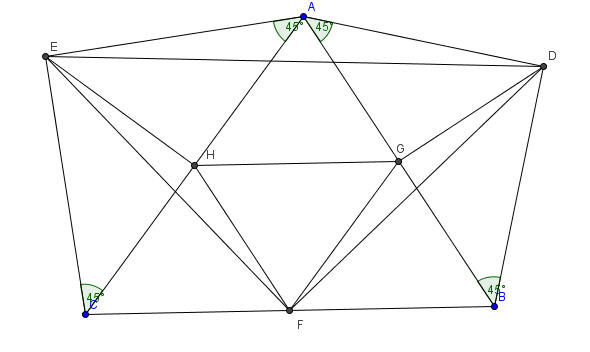
\includegraphics[scale=1]{imagenes/Geometria/20.png}
          \end{center}
          Digamos que $H$ y $G$  son los puntos medios de los segmentos $CA$ y $AB$ respectivamente y tracemos los segmentos $EH$ y $GD$, luego los $\triangle EAH,\triangle EHC,\triangle ADG$ y $\triangle DGB$ son isósceles de base $EA,EC,AD$ y $BD$ respectivamente.
          Tracemos los segmentos $HG,HF$ y $GF$, que son las paralelas medias del $\triangle ABC$, ya que $H,G$ y $F$ son puntos medios de los lados del $\triangle ABC$:
          $$\Rightarrow AG=HF$$
          y
          $$\Rightarrow HA=GF$$
          Pero tenemos que:
          $$EH=HA$$
          y
          $$DG=GA$$
          ser lados de dos triángulos isoréctangulos.
          $$\Rightarrow AG=HF=GD$$
          y
          $$\Rightarrow HA=GF=EH$$
          Por ser ángulos correspondientes tenemos que:
          $$\angle CAB=\angle CHF$$
          y
          $$\angle CAB=\angle FGB$$
          $$\Rightarrow\angle FGB=\angle CHF$$
          Por suma de ángulos tenemos que:
          $$\angle EHF=\angle EHC+\angle CHF$$
          $$\angle EHF=90^0+\angle CHF$$
          y
          $$\angle DGF=\angle DGB+\angle BGF$$
          $$\angle DGF=90^0+\angle BGF$$
          $$\Rightarrow\angle DGF=\angle EHF$$
          Luego como $HF=GD,GF=EH$ y $\angle DGF=\angle EHF$ tenemos que $\triangle EHF=\triangle FGD$ por tener dos lados y el ángulo comprendido respectivamente iguales:
          $$EF=FD$$
          por ser elementos homólogos de los $\triangle EHF$ y $\triangle FGD$. Esto nos dice que el $\triangle EDF$ es isósceles de base $ED$.
          Tenemos que:
          $${HE\over EA}=\sqrt{2}$$
          y
          $${GD\over DA}=\sqrt{2}$$
          por ser hipotenusa y cateto de dos triángulos isoréctangulos.
          $$\Rightarrow{HE\over EA}={HE\over EA}=\sqrt{2}$$
          Por suma de ángulos tenemos que:
          $$\angle EAD=\angle EAC+\angle CAB+\angle BAD$$
          $$\angle EHF=90^0+\angle CAB$$
          $$\Rightarrow\angle EHF=\angle CAB$$
          Luego como $EA$ y $AD$ son proporcionales a $HE$ y a $HF$ respectivamente y $\angle EHF=\angle CAB$ tenemos que $\triangle EHF\sim\triangle EAD$ por tener dos lados proporcionales y el ángulo comprendido respectivamente igual. Con razón de semejanza de $\sqrt{2}$:
          $${ED\over EF}=\sqrt{2}$$
          por ser elementos homólogos de los $\triangle EHF$ y $\triangle EAD$.\\
          $\therefore$ Como el $\triangle EDF$ es isósceles y la razón entre su base $ED$ y los lados iguales es igual a $\sqrt{2}$ entonces el $\triangle DEF$ es isorectángulo $\blacksquare$\\
    \item Sea el $\triangle ABC$  y $O$ su circuncentro, se trazan las alturas $AD, BE$ y $CG$, que se cortan en $K$. Sea $F$ un punto en $AB$ tal que $OF \| BC$, y $M$ el punto medio de $KM$. Halle la amplitud del $\angle FMC$.\\
          Respuesta:\\
          Demostremos el siguiente Lema:
          La distancia desde el ortocentro el triángulo a un vértice es el doble de la distancia del circuncentro al lado opuesto a dicho vértice.\\
          Luego tenemos un $\triangle ABC$ donde $H$ es el hortocentro, $O$ el circuncentro, $AD$ altura, $N$ punto medio de $AH$ y $M$ es el pie de la altura trazada desde $O$ a $BC$.\\
          Prolonguemos $AD$ hasta que corte con el circuncírculo y llamemos a ese punto $X$ y tracemos los segmentos $CX$ y $BX$.
          \begin{center}
              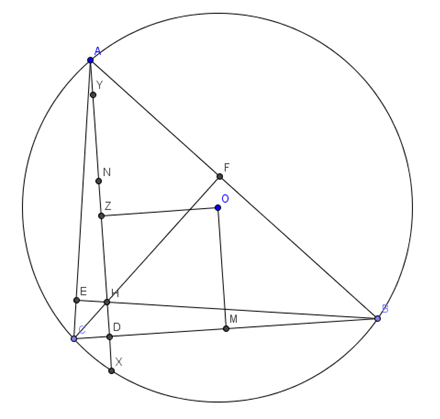
\includegraphics[scale=1]{imagenes/Geometria/21,1.png}
          \end{center}
          Luego se cumple que:
          $$\triangle ABD\sim\triangle BGC$$
          $$\Rightarrow{BC\over GC}={AB\over AD} \; (1)$$
          por ser elementos homólogos.\\
          Como $M$ es el punto medio de la hipotenusa del $\triangle BKA$, entonces es también el circuncentro de dicho triángulo, luego:
          $$\Rightarrow GM=MA$$
          $$\Rightarrow\angle GAM=\angle MGA$$
          Tenemos que:
          $$\angle GAM+\angle ABD=90^0$$
          $$\angle MGA+\angle MGK=90^0$$
          por ser ángulos complementarios.
          $$\Rightarrow\angle ABD=\angle MGK$$
          Por suma de ángulos interiores de un triángulo tenemos que:
          $$\angle CAD+\angle ACD=90^0$$
          $$\angle EBC+\angle ECB=90^0$$
          $$\Rightarrow\angle CAD=\angle EBC$$
          y
          $$\angle DAB+\angle ABD=90^0$$
          $$\angle FCB+\angle CBF=90^0$$
          $$\Rightarrow\angle DAB=\angle FCB$$
          Pero además tenemos que:
          $$\angle CAD=\angle CBX$$
          y
          $$\angle DAB=\angle BCX$$
          por ser ángulos inscritos sobre el mismo arco.
          $$\Rightarrow\angle DAB=\angle BCX=\angle FCB$$
          $$\Rightarrow\angle CAD=\angle CBX=\angle EBC$$
          Ahora como $\angle CBX=\angle EBC$, $\angle BCX=\angle FCB$ y $CB$ lado común se cumple que $\triangle CHB=\triangle CBX$ por tener dos lados y el ángulo comprendido respectivamente iguales:
          $$HD=DX$$
          por ser elementos homólogos.
          \begin{center}
              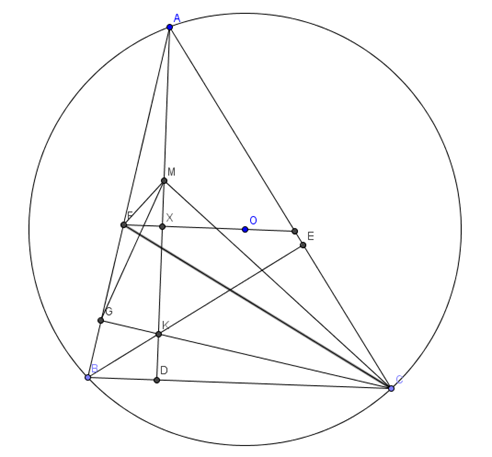
\includegraphics[scale=1]{imagenes/Geometria/21,2.png}
          \end{center}
          Ubiquemos dos puntos $Y$ y $Z$ en $AD$ de tal forma que $AY=DX=HD$ y $OZ\perp AD$.\\ Luego tenemos que:
          $$DA=AH+HD$$
          y
          $$DA=YD+AY$$
          $$\Rightarrow YD=AH$$
          Pero como $O$ es circuncentro se cumple que:
          $$ZD=OM$$
          y
          $$XZ=ZA$$
          $$AY+YZ=ZD+DX$$
          $$\Rightarrow YZ=ZD=OM$$
          Por tanto tenemos $AH=YD=YZ+ZD=2\cdot OM$. Con lo que queda demostrado el lema.\\
          Ahora apliquemos el lema al ejercicio:
          $$\Rightarrow AM=XD$$
          Por el teorema de las transversales tenemos que:
          $${FB\over AB}={XD\over AD}$$
          $${FB\over XD}={AB\over AD}\;(2)$$
          Sustituyendo (1) en (2):
          $${FB\over XD}={BC\over GC}$$
          $${FB\over BC}={AM\over GC}$$
          $$\Rightarrow{FB\over BC}={MG\over GC}$$
          Ahora como ${FB\over BC}={MG\over GC}$   y $\angle FBC=\angle MGC$ se cumple que $\triangle FBC\sim\triangle MGC$ por tener dos lados proporcionales y el ángulo comprendido respectivamente igual.
          $$\Rightarrow\angle GFC=\angle GMC$$
          por ser elementos homólogos.\\
          Esto nos dice que el cuadrilátero $FGCM$ el cíclico:
          $$\angle FGC+\angle FMC=180^0$$
          $$\angle FMC=90^0$$
          $\therefore$ La amplitud del $\angle FMC$ es de $90^0$  $\blacksquare$\\
    \item Se tiene un $\triangle ABC$ sea $G$ el baricentro y $O$ el circuncentro de dicho triángulo, $AH \bot BC$ y $I$ un punto medio de $AH$ sea $L$ el punto de intersección del circuncírculo del $\triangle ABC$ con $GH$ y sea $T$ el circuncentro del $\triangle BTH$. Pruebe que $AO$ y $BT$ se cortan sobre el circuncírculo del $\triangle ABC$. \\
          Respuesta:
          \begin{center}
              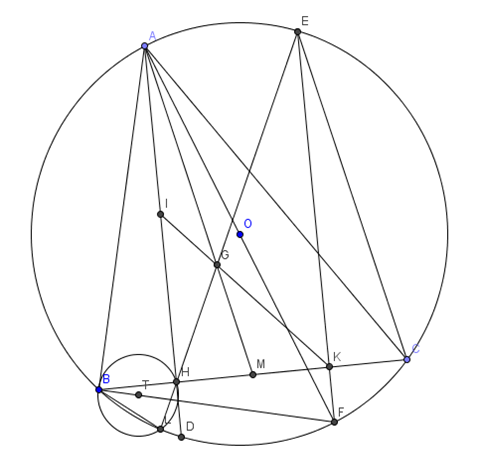
\includegraphics[scale=1]{imagenes/Geometria/22.png}
          \end{center}
          Llamemos $K$ y $M$ a la intersección de $BC$ y $IG$ y a la intersección de $AG$ y $BC$ respectivamente:
          $$\Rightarrow{2GA\over 3}=GM$$
          porque $G$ es el baricentro del $\triangle ABC$. Pero tenemos que $IK$ es mediana de $AH$, luego como $IK$ pasa por $G$ y este punto se ubica en la razón  $\displaystyle{{2\over 3}}$  sobre el segmento $AM$, entonces se cumple que $G$ es también el baricentro del $\triangle AHK$:
          $$\Rightarrow MH=HK$$
          pero como $BM=MC\Rightarrow BH=KC$ por sustracción de segmentos.\\
          Prolonguemos HA hasta tocar la circunferencia en $D$ y tracenos la perpendicular a $BC$ por $K$ que corta a la circunferencia en $E$ y $F$. Luego como $BH=CK$ se cumple por simetría que $EF=AD$ y teníamos que $EF\parallel AD$ entonces $ADFE$ es un paralelogramo pero los únicos paralelogramos cíclicos son los rectángulos, esto nos dice que $ADFE$ es un rectángulo:\\
          $$\Rightarrow DF\parallel BC\parallel AE$$
          Digamos que:
          $$P=AK\cap GH$$
          $$\Rightarrow AP=PH=KP$$
          ya que $G$ es el baricentro $\triangle AKH$ es rectángulo.\\
          Luego $AK$ y $HE$ se cortan en su punto medio por ser diagonales de un rectángulo y $P$ es punto medio de $AK$, lo cual implica que $P$ es también punto medio de $HE$, por tanto $H$,$G$ y $E$ están alineados:
          $$\Rightarrow{\stackrel{\textstyle\frown}{\mathrm{BE}}\over 2}=\angle BLH$$
          $${\stackrel{\textstyle\frown}{\mathrm{CA}}\over 2}=\angle ABC$$
          por inscritos sobre el mismo arco.\\
          Como $BC\parallel AE$ y son cuerdas de la circunferencia se cumple que $AECB$ es un trapecio isósceles:
          $$\Rightarrow AC=BK$$
          por ser diagonales de un trapecio isósceles.
          $$\Rightarrow\angle BLH=\angle ABC$$
          porque a cuerdas iguales, ángulos inscritos iguales.\\
          Ahora en el circuncículo del $\triangle BLH$ se cumple que el $\angle BLH$ es seminscrito sobre $\stackrel{\textstyle\frown}{\mathrm{BH}}$ y el $\angle ABC$ está en posición de seminscrito sobre este mismo arco, luego se cumple que $AB$ es tangente al circuncículo del $\triangle BLH$.\\
          $\therefore$ $BT\perp AB$ por propiedad de la tangente y por el teorema de Tales la perpendicular a $AB$ corta al diámetro $AO$ en el circuncículo del $\triangle ABC$. Con lo cual queda probado $\blacksquare$\\
    \item Se tiene un $\triangle ABC$ y se trazan las alturas $BD$ y $CE$, cortándose en $H,DE$ y $BC$ se intersecan en $F$, $IA$ es la mediana relativa a $BC$.
          \begin{enumerate}
              \item Demuestre que $ID$ y $IE$ son tangentes al circuncírculo del $\triangle ADE$.
              \item Demuestre que $IA \bot FH$.
          \end{enumerate}
          Respuesta:
          \begin{enumerate}
              \item Como $DB$ y $CE$ son alturas tenemos que:
                    $$\angle CDB=\angle CEB=90^0$$
                    Luego se cumple que el cuadrilátero $BEDC$ es cíclico, pero como $I$ es el pnto medio de $BC$ y $\angle CDB=\angle CEB=90^0$ entoces $I$ es el centro del circuncírculo del cuadrilátero $BEDC$:
                    $$\Rightarrow ID=IE$$
                    por ser radios.
                    $$\angle IDE=\angle IED$$
                    Ahora por ser ángulo exterior a la circunferencia tenemos que:
                    $$\angle CAB={\stackrel{\textstyle\frown}{\mathrm{CB}}\over 2}-{\stackrel{\textstyle\frown}{\mathrm{DE}}\over 2}$$
                    $$\angle CAB=90^0-{\stackrel{\textstyle\frown}{\mathrm{DE}}\over 2}$$
                    Pero por ser un ángulo central tenemos que:
                    $$\angle DIE=\stackrel{\textstyle\frown}{\mathrm{DE}}$$
                    Por suma de ángulos interiores de un triángulo se tiene que:
                    $$\angle IDE+\angle DIE+\angle DEI=180^0$$
                    $$\angle IED=90^0-{\stackrel{\textstyle\frown}{\mathrm{DE}}\over 2}$$
                    $$\Rightarrow\angle IED=\angle CAB$$
                    $\therefore$ $IE$ y $ID$ son tangentes al circuncírculo del $\triangle DAE$ ya que el ángulo inscrito y el seminscrito son iguales $\blacksquare$
                    \begin{center}
                        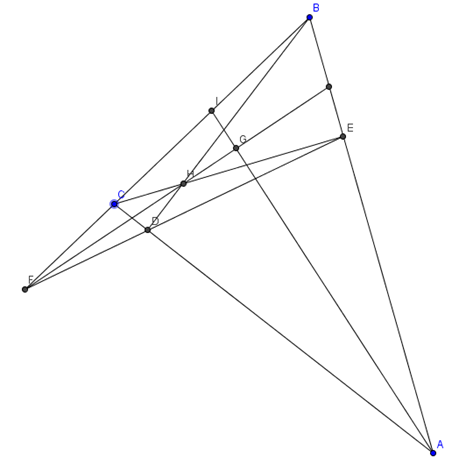
\includegraphics[scale=1]{imagenes/Geometria/23.png}
                    \end{center}
              \item Por ser ángulos opuestos de un cuadrilátero cíclico tenemos que:
                    $$\angle CAB=180^0-\angle DHA$$
                    Pero por ángulos adyacentes tenemos que:
                    $$\angle CHD=180^0-\angle DHA$$
                    $$\Rightarrow\angle CAB=\angle CHD=x$$
                    Llamemos $\alpha=\angle CHD$, $\beta=\angle FHD$, $\gamma =\angle IAE$ y $\theta=\angle IAC$.\\
                    Apliquemos la ley de los senos:
                    $${\sen \alpha\over FC}={\sen {\angle HCF}\over FH}$$
                    y
                    $${\sen \beta\over FD}={\sen {\angle FDH}\over FH}$$
                    Pero por ser ángulos adyacentes tenemos que:
                    $$\sen {\angle HFC}=\sen {\angle HBC}$$
                    y
                    $$\sen {\angle HDF}=\sen {\angle HDE}$$
                    Luego como $\angle HDE=\angle HCB$ por estar inscritos sobre el mismo arco:
                    $$\Rightarrow\sen {\angle HDF}=\sen {\angle HCF}$$
                    $$\Rightarrow{\sen {\angle HCF}\over FH}={\sen {\angle FDH}\over FH}$$
                    $$\Rightarrow{\sen \alpha\over FC}={\sen \beta\over FD}$$
                    $${\sen \alpha\over\sen \beta}={FC\over FD}$$
                    Apliquemos la ley de los senos:
                    $${\sen {\angle DCF}\over FD}={\sen {\angle FDC}\over FC}$$
                    $${\sen {\angle FDC}\over\sen {\angle DCF}}={FC\over FD}$$
                    $$\Rightarrow{\sen \alpha\over\sen \beta}={\sen {\angle FDC}\over\sen {\angle DCF}}$$
                    Ahora se cumple que:
                    $$\angle FCD=180^0-\angle DCB$$
                    $$\sen {\angle BED}=\sen {\angle DEA}$$
                    por ser ángulos adyacentes.\\
                    Pero se tiene que:
                    $$\angle BED=180^0-\angle DCB$$
                    por ser ángulos opuestos de un cuadrilátero cíclico.
                    $$\Rightarrow\angle FCD=\angle BED$$
                    Luego tenemos que:
                    $$\sen {\angle BED}=\sen {\angle DEA}$$
                    por ser ángulos adyacentes.
                    $$\Rightarrow\sen {\angle FCD}=\sen {\angle DEA}$$
                    Por ser ángulos alternos por el vértice tenemos que:
                    $$\angle CDF=\angle EDA$$
                    Ahora por transitividad se tiene que:
                    $${\sen \alpha\over\sen \beta}={\sen {\angle FDC}\over\sen {\angle DCF}}={\sen {\angle EDA}\over\sen {\angle DEA}}$$
                    Apliquemos ley de los senos:
                    $$\sen {\angle EDA}\over\sen {\angle DEA}={EA\over DA}$$
                    Por potencia del punto A tenemos que:
                    $$EA\cdot AB=AD\cdot CD$$
                    $${EA\over DA}={CA\over AB}$$
                    $$\Rightarrow{\sen \alpha\over\sen \beta}={EA\over DA}={CA\over AB}$$
                    Apliquemos nuevamente la ley de los senos:
                    $${\sen \gamma\over IB}={\sen {\angle BIA}\over BA}$$
                    y
                    $${\sen \theta\over IC}={\sen {\angle CIA}\over CA}$$
                    Dividiendo las dos ecuaciones:
                    $${\sen \gamma\over IB}\cdot{IC\over\sen \theta}={\sen {\angle BIA}\over BA}\cdot{CA\over\sen {\angle CIA}}$$
                    $$\Rightarrow{\sen \gamma\over\sen \theta}={CA\over AB}$$
                    $$\Rightarrow{\sen \gamma\over\sen \theta}={\sen \alpha\over\sen \beta}$$
                    Pero tenemos que:
                    $$x=\alpha+\beta=\gamma+\theta$$
                    Sustituyendo:
                    $${\sen {x-\theta}\over\sen \theta}={\sen {x-\beta}\over\sen \beta}$$
                    $$\frac{\sen x\cdot\cos \theta}{\sen \theta}-\frac{\cos x\cdot\sen \theta}{\sen \theta}=\frac{\sen x\cdot\cos \beta}{\sen \beta}-\frac{\cos x\cdot\sen \beta}{\sen \beta}$$
                    $$\sen x\cdot\cot \theta-\cos x=\sen \beta\cdot\cot \beta-\cos x$$
                    $$\cot \theta=\cot \beta$$
                    $$\Rightarrow\theta=\beta$$
                    ya que son ángulos del primer cuadrante.\\
                    Luego:
                    $$\theta=\beta\wedge\alpha=\beta$$
                    Digamos que $G=AI\cap FH$
                    $$\angle GHE=\alpha$$
                    por opuestos por el vértice.
                    $$\Rightarrow\angle GAE=\angle GHE=\alpha$$
                    luego $GHEA$ es cíclico porque los ángulos inscritos son iguales.\\
                    $\therefore$ $\angle HEA=\angle AGH=90^0$ por estar inscritos sobre el mismo arco $\blacksquare$\\
          \end{enumerate}
    \item En el $\triangle ABC$ equilátero se inscribe una circunferencia. Demostrar que para todos los puntos $P$ de la circunferecia, el área del triángulo formado por los lados cuyas longitudes son $PA, PB$ y $PC$ es $\displaystyle{\frac{1}{4}}$ del área del $\triangle ABC$. \\
          Respuesta:\\
          Digamos que el lado de triángulo es $6a$ .Construyamos un $\triangle ABD$ equilátero y supongamos que $A=C$,$D=A$ y $B=B$, ahora ubiquemos un punto $Q$ en la circunferencia circunscrita al $\triangle ABD$ de manera que el nuevo triángulo obtenido y todos sus elementos interiores son iguales.
          Ahora como para ubicar el punto $Q$, primero supusimos que $A=C$,$D=A$ y $B=B$, por simetría tenemos que: $AQ=CP$,$BQ=BP$ y $DQ=AP$, pero también se cumple que: $\triangle ADQ=\triangle CAP$,$\triangle ABQ=\triangle CBP$ y $\triangle DBQ=\triangle ABP$.
          \begin{center}
              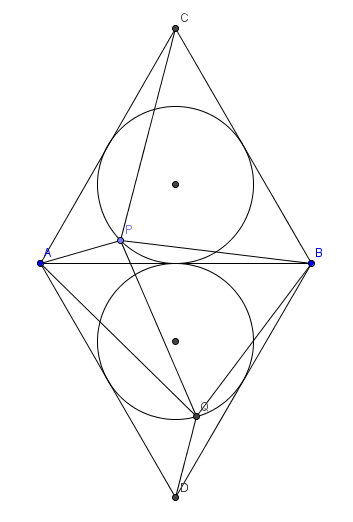
\includegraphics[scale=1]{imagenes/Geometria/24,1.png}
          \end{center}
          Entonces por elementos homólogos tenemos que:
          $$\angle CBP=\angle ABQ$$
          $$\angle PBA=\angle QBD$$
          Ahora por suma de ángulos se tiene que:
          $$\angle PBQ=\angle PBA+\angle ABQ$$
          $$\angle PBQ=\angle PBA+\angle CBP$$
          $$\Rightarrow\angle PBQ=\angle CBA$$
          $$\angle PBQ=60^0$$
          Entonces como $\angle PBQ=60^0$ y $BQ=BP$, entonces el $\triangle BPQ$ es equilátero:
          $$\Rightarrow PQ=PB$$
          Ahora démonos cuenta que el triángulo buscado es el $\triangle APQ$, ya que $PQ=PB$ y $AQ=PC$.\\
          Denotemos $(MNOPQ)$ como área del polígono del $MNOPQ$.
          Luego por suma de área tenemos que:
          $$(APC)+(PCB)+(APQ)+(AQD)+(PQB)+(DQB)=(ABC)+(ABD)$$
          $$(APC)+(PCB)+(APQ)+(APC)+{PB^2\sqrt{3}\over 4}+(APB)=2(ABC)$$
          $$(APQ)+(APC)+(ABC)+{PB^2\sqrt{3}\over 4}=2(ABC)$$
          $$(APQ)+(APC)+{PB^2\sqrt{3}\over 4}=(ABC)$$
          De manera análoga si hacemos el mismo procedimiento con los lados $BC$ y $AC$, obtendremos:
          $$(APQ)+(APB)+{PA^2\sqrt{3}\over 4}=(ABC)$$
          $$(APQ)+(BPC)+{PC^2\sqrt{3}\over 4}=(ABC)$$
          Sumando estas tres ecuaciones tenemos que:
          $$3(APQ)+(APC)+(APB)+(BPC)+{PB^2\sqrt{3}\over 4}+{PA^2\sqrt{3}\over 4}+{PC^2\sqrt{3}\over 4}=3(ABC)$$
          $$3(APQ)+{\sqrt{3}\over 4} (PB^2+PA^2+PC^2 )=2(ABC)$$
          Ahora hallemos el valor de $PB^2+PA^2+PC^2$, para ello ubiquemos el $\triangle ABC$ en un sistema de coordenadas con centro en el centro de la circunferencia inscrita. Luego aplicando las proporciones correspondientes del triángulo equilátero llegamos a que:
          $$A=0 ;2a\sqrt{3}$$
          $$B=3a ; -a\sqrt{3}$$
          $$C=-3a ; -a\sqrt{3}$$
          Luego la ecuación de la circunferencia circunscrita sería:
          $$x^2+y^2=3a^2$$
          Ahora digamos que el punto P tiene coordenadas (m ; n), entonces:
          $$m^2+n^2=3a^2$$
          Hallemos las longitudes de los segmentos $PA$, $PB$ y $PC$:
          $$PA=\sqrt{m^2+{\big(n-2a\sqrt{3}\big)}^2 }$$
          $$PA^2=m^2+n^2-4n2a\sqrt{3}+12a^2$$
          $$PB=\sqrt{{(m-3a)}^2+{\big(n+a\sqrt{3}\big)}^2 }$$
          $$PB^2=m^2-6ma+9a^2+n^2+2na\sqrt{3}+3a^2$$
          $$PC=\sqrt{{(m+3a)}^2+{\big(n+a\sqrt{3}\big)}^2 }$$
          $$PC^2=m^2+6ma+9a^2+n^2+2na\sqrt{3}+3a^2$$
          \begin{center}
              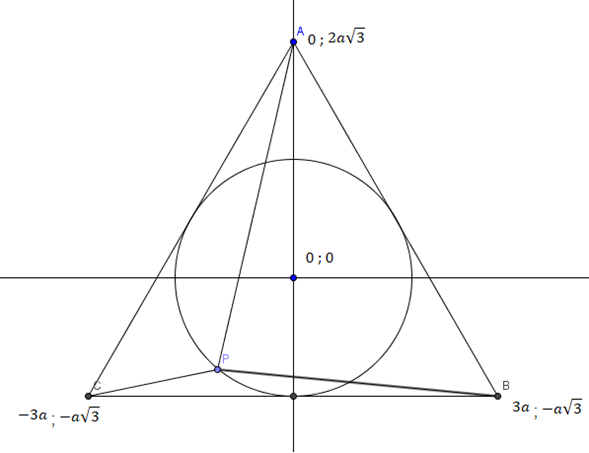
\includegraphics[scale=1]{imagenes/Geometria/24,2.png}
          \end{center}
          Sumando miembro a miembro:
          $$PB^2+PA^2+PC^2=m^2+n^2-4n2a\sqrt{3}+12a^2+m^2-6ma+9a^2+n^2+2na\sqrt{3}+3a^2+m^2+6ma+9a^2+n^2+2na\sqrt{3}+3a^2$$
          $$PB^2+PA^2+PC^2=3m^2+3n^2+36a^2$$
          $$PB^2+PA^2+PC^2=9a^2+36a^2$$
          $$PB^2+PA^2+PC^2=45a^2$$
          Ahora sustituyendo:
          $$3(APQ)+{\sqrt{3}\over 4}45a^2=2\cdot 36a^2  {\sqrt{3}\over 4}$$
          $$(APQ)=9a^2 {\sqrt{3}\over 4}$$
          Calculemos:
          $$\frac{(APQ)}{(ABC)}=\frac{9a^2  {\sqrt{3}\over 4}}{36a^2  {\sqrt{3}\over 4}}$$
          $$\frac{(APQ)}{(ABC)}={1\over 4}$$
          $\therefore$ Se cumple que para todos los puntos $P$ de la circunferecia, el área del triángulo formado por los lados cuyas longitudes son $PA, PB$ y $PC$ es $\displaystyle{\frac{1}{4}}$ del área del $\triangle ABC$ $\blacksquare$\\
    \item Sea un $\triangle ABC$ y $\omega$ su circuncírculo. Las tangentes a $\omega$ en $B$ y $C$ se cortan en $T$. Sea $S$ un punto sobre $BC$ tal que $AS \bot AT$. $D$ y $E$ son puntos sobre la recta $ST$ (con $E$ entre $D$ y $S$) tal que $DT = BT =ET$. Pruebe que el $\triangle ABC\sim\triangle ADE$. \\
          Respuesta:
          \begin{center}
              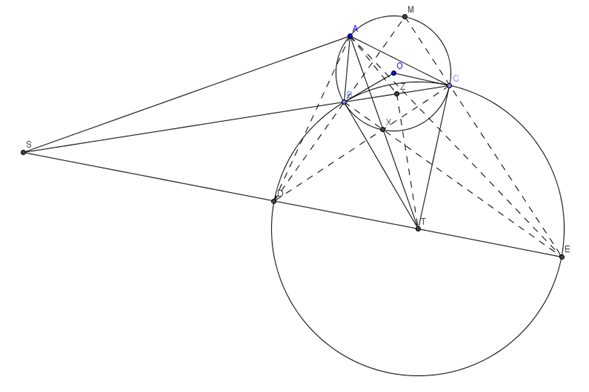
\includegraphics[scale=1]{imagenes/Geometria/25,1.png}
          \end{center}
          Llamemos $X$ a la intersección de $BE$ y $CD$ y $Z$ al punto medio del segmento $BC$.\\
          Digamos que:
          $$\angle TBD=\angle TDB=a$$
          $$\angle ECT=\angle TEC=b$$
          $$\angle TBC=\angle TCB=k$$
          por ser ángulos bases de un triángulo equilátero.\\
          Ahora por suma de ángulos interiores de un triángulo se cumple que:
          $$\angle BTC=180^0-2k$$
          $$\angle BTD=180^0-2a$$
          $$\angle CTE=180^0-2b$$
          Sumando estas tres ecuaciones tenemos que:
          $$\angle BTC+\angle BTD+\angle CTE=540^0-2(a+b+k)$$
          $$a+b+k=180^0$$
          Digamos que $DB$ y $CE$ se cortan en $M$. Luego por suma de ángulos interiores de un triángulo se cumple que:
          $$\angle MDE+\angle MED+\angle DME=180^0$$
          $$\angle DME=180^0-a-b$$
          $$\angle DME=k$$
          $$\Rightarrow\angle BMC=\angle BCT=k$$
          Entonces como $\angle BCT$ es seminscrito y el $\angle BMC$ está en posición de inscrito $\Rightarrow M\in\omega$.\\
          Como $BT=DT=CT=ET$ entonces el cuadrilátero $BDCE$ es cíclico, luego por el teorema de Tales se cumple que los $\omega BDE$ y $\omega CDE$ son triángulos rectángulos.\\
          Entonces por ser ángulos complementarios tenemos que:
          $$\angle BED+\angle BDE=90^0$$
          $$\angle BED=90^0-a$$
          y
          $$\angle CDE+\angle CED=90^0$$
          $$\angle CDE=90^0-b$$
          Luego se cumple que:
          $$\angle BCD=\angle BED=90^0-a$$
          $$\angle CBE=\angle CDE=90^0-b$$
          por estar inscritos sobre el mismo arco.\\
          Ahora por suma de ángulos interiores de un triángulo se cumple que:
          $$\angle BCX+\angle BXC+\angle CBX=180^0$$
          $$\angle BCX=180^0-90^0+a-90^0+b$$
          $$\angle BCX=a+b=180^0-k$$
          $$\Rightarrow\angle BCX+\angle BMC=180^0-k+k=180^0$$
          $$\Rightarrow X\in\omega$$
          Como el $\triangle BTC$ es isósceles de base $BC$ y $Z$ es el punto medio de este segmento, entonces $\angle BZT=90^0$.\\
          Luego como $\angle BZT=\angle SAT=90^0$ se cumple que el cuadrilátero $AZTS$ es cíclico porque los ángulos que están en posición de inscritos son iguales.\\
          Ahora el $\angle CSE$ es exterior al circuncírculo $BCED$ por lo que:
          $$\angle CSE={\stackrel{\textstyle\frown}{\mathrm{EC}}\over 2}-{\stackrel{\textstyle\frown}{\mathrm{BD}}\over 2}=90^0-b-90^0+a=a-b$$
          Luego:
          $$\angle BAC=k$$
          $$\angle TAZ=\angle ZST=a-b$$
          $$\angle BAX=\angle BCX=90^0-a$$
          por estar inscritos sobre el mismo arco.\\
          %Aqui empieza la demostracion del lema de la simediana---------------------------------------------------
          Demostremos el siguiente lema, se tiene un $MNL$ inscrito en una circunferencia, por $N$ y $L$ se trazan las tangentes que se cortan en $P$, luego $MP$ es la simediana correspondiente al lado $NL$:\\
          Nota: La simediana es la recta es la recta que se obtiene al reflejar la mediana por la bisectriz.
          Para probar el lema solo basta probar que: $\angle LMP=\angle QMN$, siendo $Q$ el punto medio de $NL$.
          \begin{center}
              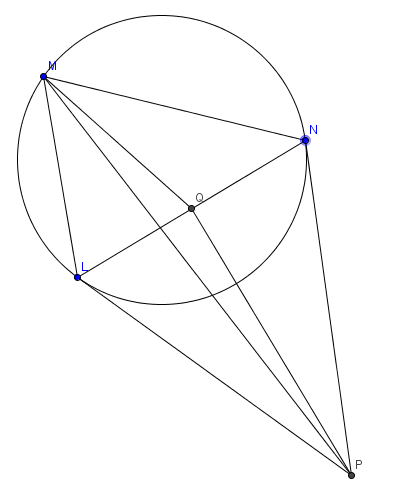
\includegraphics[scale=1]{imagenes/Geometria/25,2.png}
          \end{center}
          Apliquemos la ley de los senos:
          $${\sen {\angle QMN}\over QN}={\sen {\angle MNQ}\over MQ}$$
          $${\sen {\angle QML}\over QL}={\sen {\angle MLQ}\over MQ}$$
          Dividiendo las dos ecuaciones:
          $$\frac{\sen {\angle QMN}\cdot QL}{\sen {\angle QML}\cdot QN}=\frac{\sen {\angle MNQ}\cdot MQ}{\sen {\angle MLQ}\cdot MQ}$$
          $$\frac{\sen {\angle QMN}}{\sen {\angle QML}}=\frac{\sen {\angle MNQ}}{\sen {\angle MLQ}}$$
          $$\angle LMN=\angle NLP=\angle PNM$$
          por estar inscrito y seminscrito sobre el mismo arco.\\
          Apliquemos la ley de los senos:
          $${\sen {\angle PMN}\over NP}={\sen {\angle MNP}\over MP}$$
          $${\sen {\angle PML}\over LP}={\sen {\angle MLP}\over MP}$$
          Dividiendo las dos ecuaciones:
          $$\frac{\sen {\angle PMN}\cdot LP}{\sen {\angle PML}\cdot NP}=\frac{\sen {\angle MNP}\cdot MP}{\sen {\angle MLP}\cdot MP}$$
          $${\sen {\angle PMN}}{\sen {\angle PML}}=\frac{\sen {(\angle MNL+\angle LNP)}}{\sen {(\angle MLN+\angle NLP)}}$$
          Pero como $\angle MNL+\angle MLN+\angle LMN=180^0$ por suma de ángulos interiores de un triángulo:
          $$\frac{\sen {\angle PMN}}{\sen {\angle PML}}=\frac{\sen {\angle MLN}}{\sen {\angle MNL}}$$
          $$\Rightarrow\frac{\sen {\angle PMN}}{\sen {\angle PML}}=\frac{\sen {\angle QML}}{\sen {\angle QMN}}$$
          $$\frac{\sen {(\angle NML-\angle PML)}}{\sen {\angle PML}}=\frac{\sen {(\angle NML-\angle QMN)}}{\sen {\angle QMN}}$$
          $$\frac{\sen{\angle NML}\cdot\cos{\angle PML}-\cos{\angle NML}\cdot\sen{\angle PML}}{\sen{\angle PML}}=\frac{\sen{\angle NML}\cdot\cos{\angle QMN}-\cos{\angle NML}\cdot\sen{\angle QMN}}{\sen{\angle QMN}}$$
          $$\sen{\angle MNL}\cdot\cot{\angle PML}-\cos{\angle NML}=\sen{\angle MNL}\cdot\cot{\angle QMN}-\cos{\angle NML}$$
          $$\cot{\angle PML}=\cot{QMN}$$
          $$\Rightarrow\angle PML=\angle QMN$$
          ya que son ángulos del primer cuadrante. Por lo tanto queda probado el lema.\\
          Entonces de regreso al ejercicio:
          $$\angle BAT=\angle\angle ZAC$$
          por el lema que acabamos de probar, ya que $AT$ simediana.
          $$\Rightarrow\angle BAT={\angle BAC-\angle TAZ\over 2}={180^0-a-b-a+b\over 2}=90^0-a$$
          $$\Rightarrow\angle BAT=\angle BAX=90^0-a$$
          Por tanto se cumple que $A$, $T$ y $X$ están alineados.
          $$\Rightarrow\angle BAT=\angle BET=90^0-a$$
          Luego el cuadrilátero $ABTE$ es cíclico porque los ángulos que están en posición de inscritos son iguales.\\
          Ahora:
          $$\angle XBC=\angle XAC=90^0-b$$
          por estar inscritos sobre el mismo arco.\\
          Por tanto el cuadrilátero $ACTD$ es cíclico porque los ángulos que están en posición de inscritos son iguales. \\
          Pero como $TC=DT$ y $TB=TE$:
          $$\angle DAT=\angle TAC$$
          $$\angle BAT=\angle TAE$$
          por estar inscritos sobre el mismo arco.\\
          Luego:
          $$\angle DAT=\angle TAC$$
          $$\angle DAB+\angle DAT=\angle TAE+\angle EAC$$
          por suma de ángulos consecutivos.
          $$\Rightarrow\angle DAB=\angle EAC$$
          Ahora:
          $$\angle DAB+\angle BAE=\angle DAE$$
          $$\angle BAE+\angle EAC=\angle BAC$$
          por suma de ángulos consecutivos.
          $$\Rightarrow\angle DAE=\angle BAC=k$$
          Entonces el cuadrilátero $DAME$ es cíclico porque los ángulos que están en posición de inscritos son iguales.
          $$\angle ADM=\angle AEM$$
          por estar inscritos sobre el mismo arco.\\
          Luego como $\angle ADM=\angle AEM$ y $\angle DAB=\angle EAC$ se cumple $\angle ABD\sim\triangle ACE$ por tener dos ángulos respectivamente iguales.
          $${DA\over BA}={EA\over CA}$$
          por ser elementos homólogos.\\
          $\therefore$ $\triangle ABC\sim\triangle ADE$ por tener dos lados proporcionales y el ángulo comprendido respectivamente iguales $\blacksquare$\\
          
\end{enumerate}


\chapter{Combinatoria}


\section{Ejercicios (Combinatoria)}
\begin{enumerate}
    \item ¿De cuántas maneras diferentes puede un estudiante adivinar un examen completo de verdadero/falso que tenga $n$ preguntas?
    \item Considere la siguiente figura:
          \begin{center}
              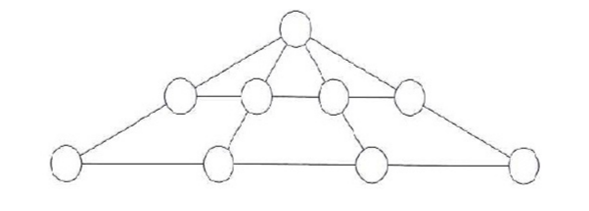
\includegraphics[scale=1]{imagenes/Combinatoria/1,1.png}
          \end{center}
          En cada círculo se pueden colocar los números del 1 al 9 y cada uno puede ser usado exactamente una vez. Las seis sumas que se pueden realizar siguiendo las lineas dibujadas son iguales (de 3 y 4 sumando).
          \begin{enumerate}
              \item Muestre que cualquier solución tiene el mismo número en el círculo de la cima.
              \item ¿Cuántas formas existen de colocar los números? (Dos formas se consideran diferentes si tienen al menos dos círculos con números diferentes)
          \end{enumerate}
    \item En un baile al cual asisten n parejas formadas por marido y mujer se presenta la siguiente situación cuando se van a sentar a una mesa rectangular que cuenta con $2n$ sillas dispuestas en fila:
          \begin{enumerate}
              \item Cada mujer se quiere sentar al lado de su marido.
              \item Las mujeres y los hombres se quieren sentar alternadamente (entre dos hombres debe haber una mujer y entre dos mujeres debe haber un hombre).
          \end{enumerate}
    \item Matematiquito tiene escrito en una pizarra los números del 1 al 2019. Luego en cada paso escoge dos números, los borra, los suma y escribe la suma de los dígitos del número obtenido. Puede que el último número que obtenga Matematiquito sea:
          \begin{enumerate}
              \item El 3.
              \item El 6.
          \end{enumerate}
    \item En un país un caso policial hay $n$ sospechosos, de manera tal que cada uno conoce a los culpables, pero se sabe que los culpables fueron los únicos que dijeron mentira en los interrogatorios. Llamemos $a_i$ al sospechoso $i$. En los interrogatorios se hizo solo una pregunta: ¿cuántos culpables hay? y estas fueron las respuestas:
          \begin{center}
              $a_1$: 1 culpable.\\
              $a_2$: 2 culpables.\\
              $\vdots$\\
              $a_i: i$ culpables.\\
              $\vdots$\\
              $a_n: n$ culpables
          \end{center}
          Ayude a resolver el caso policial determinando los criminales.
    \item Se tiene un polígono regular de $2k$ lados. ¿Qué probabilidad hay de escoger 3 vértices de este polígono y que estos formen un triángulo rectángulo?
    \item En una granja se tienen gallinas y patos en un corral de 123 x 123 unidades dividido en regiones de una unidad cuadrada y contiene un solo animal. Los animales se ubican de la siguiente forma: si una región contiene un pato(siempre que no este en el borde), la cantidad de regiones con gallinas aledañas a esta debe ser igual a 4 y si una región contiene una gallina(siempre que no este en el borde), la cantidad de regiones con patos aledañas a esta debe ser igual a 5. Halle la cantidad de gallinas y patos presentes en el corral.
    \item La máquina regala monedas funciona de la siguiente manera: cuando se introduce una moneda de 25 centavos la máquina devuelve cinco monedas de 5 centavos, cuando se introduce una moneda de 5 centavos la máquina devuelve cinco monedas de 1 centavo, cuando se introduce una moneda de 1 centavo la máquina devuelve cinco monedas de 25 centavos. Diego comienza con una sola moneda de 1 centavo. Decidir si después de usar la máquina repetidas veces puede retirarse con 745 centavos o con 907 centavos y para el total que se pueda, probar cómo lo puede lograr.
    \item Un coche de un tren tiene dos filas enfrentadas, de 5 asientos cada una, con un asiento de cada fila junto a la ventana. Hay 9 pasajeros, tres de los cuales quieren sentarse en sentido de la marcha. A los otros 6 no les importa el sentido, pero hay una madre cuyo hijo quiere sentarse junto a ella y al lado de la ventana. ¿De cuántas maneras pueden sentarse los pasajeros de forma tal que todos estén satisfechos?
    \item Matematiquito está jugando un juego con sus amigos de la siguiente manera, él tiene 100 sillas dispuestas sobre una fila y a enumeradas de 1 al 100, al principio todas las sillas están ocupadas por uno de sus amigos cada una, en la segunda ronda Matematiquito pasa parando a los que están sobre las sillas pares, en la tercera Matematiquito para o sienta a sus amigos en las sillas múltiplos de 3 y así repetidamente hasta la ronda 100. Al final del juego cuáles sillas quedarán ocupadas.
    \item Matematiquito y Matematiquita juegan alternadamente, comenzando por Matematiquito, coloreando segmentos sobre la siguiente figura, formada por triangulitos equiláteros iguales:
          \begin{center}
              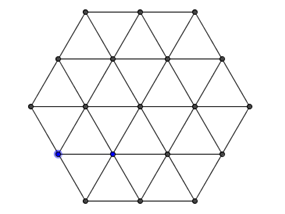
\includegraphics[scale=1]{imagenes/Combinatoria/11.png}
          \end{center}
          Las reglas del juego son las siguientes: los segmentos deben estar sobre los lados de los triangulitos, se pueden colorear los segmentos que no tengan ningún punto en común con los segmentos ya coloreados incluyendo a los extremos y por último pierde el que no pueda colorear más ningún segmento. Muestre que uno de los dos tiene una estrategia ganadora y descríbala.
    \item Los números $a_1,a_2,\ldots ,a_{n^2}$ se colocan en un tablero de $n$ x $n$ de tal manera que los elementos ubicados sobre cada fila y sobre cada columna formen una progresión aritmética. Halle la suma de los elementos ubicados en las esquinas del tablero.
    \item Se tiene un tablero de $n$ x $n$ rellenado con los números desde el 1 hasta $n^2$, para cada fila y cada columna se calcula la diferencia entre el mayor y el menor elemento. Sea $S$ la suma de los 4096 números obtenidos. Halle el máximo valor de $S$.
    \item Matematiquito y Matematiquita juegan alternadamente sobre la cuadricula dada. Cada uno en su turno traza de 1 a 5 recorridos diferentes a los trazados anteriormente, que unan A con B, moviéndose únicamente a la derecha y hacia arriba sobre las líneas de la cuadricula. Juan empieza jugando. Pierde el que trace un recorrido que pase por C o D. Prueba que uno de ellos puede ganar independientemente de como juegue el otro.
          \begin{center}
              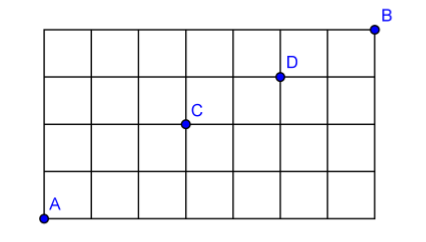
\includegraphics[scale=1]{imagenes/Combinatoria/13.png}
          \end{center}
    \item Matematiquito y Matematiquita inician un juego donde alternadamente van sustituyendo el número escrito en la pizarra. En cada turno, el jugador debe sustituir el número escrito, ya sea por la cantidad de divisores del número escrito o por la diferencia entre el número escrito y su cantidad de divisores. Matematiquito es el primero en jugar, y el que escriba el cero gana. Dado que el número inicial es 1036, determine qué jugador tiene una estrategia ganadora y enúnciela.
    \item En la pizarra está escrito el número 3. Matematiquito y Matematiquita juegan alternadamente, comenzando Matematiquito, de la manera siguiente: si en la pizarra está escrito el número $n$, el jugador que tenga el turno lo debe sustituir por cualquier entero $m$ que sea primo relativo con $n$ y tal que $n<m<n^2$. El primer jugador que escriba un número mayor o igual a 2016 gana. Determine qué jugador tiene una estrategia ganadora y enúnciela.
    \item Un conjunto $X$ de enteros positivos es ibérico si $X$ es un subconjunto de {2,3,4,...,3141592653589} y siempre que $m$ y $n$ pertenezcan a $X$, entonces el $mcd(m,n)$ pertenece también a $X$. Un conjunto ibérico es olímpico si no está contenido en ningún otro conjunto ibérico. Encontrar todos los conjuntos ibéricos olímpicos que contienen el número 2020.
    \item Sea $n$ un entero positivo. Para una permutación $a_1,a_2,\ldots ,a_n$ de los números $1,2,\ldots ,n$ , definimos:
          
          $$b_k=\min_{1\leq i\leq k}a_i+\max_{1\leq j\leq k} a_j$$
          para cada $k = 1,2,\ldots ,n$. \\
          Decimos que la permutación $a_1,a_2,\ldots ,a_n$ es guadiana si la sucesión $b_1,b_2,\ldots ,b_n$ no tiene dos elementos consecutivos iguales. ¿Cuántas permutaciones guadianas existen?
    \item Se tiene un polígono regular $P$ con $2n+1$ vértices y en cada vértice hay un caramelo. Dos jugadores Matematiquita y Matematiquito van a jugar alternadamente empezando por Matematiquita, con las siguientes reglas. Primero Matematiquita elige un triángulo con vértices en $P$ y coloca en el interior del triángulo el número 1, después Matematiquito elige un triángulo con vértices en $P$ y coloca en el interior del triángulo el número 2, de tal forma que los triángulos elegidos en cada jugada no se intersecan en su interior con los anteriores. Continúan así hasta que no pueden realizar más jugadas. Después el caramelo que hay en cada vértice lo gana el jugador que tenga más triángulos con su número incidiendo en ese vértice, si la cantidad de triángulos incidentes en un vértice es la misma para los dos jugadores el caramelo no se lo lleva nadie y sale del juego. Gana el jugador que más caramelos acumule. Determine el jugador que siempre puede lograr la victoria y describa su estrategia.\\
          Nota: Los triángulos pueden compartir lados y vértices.
    \item Un polígono regular de $n$ lados $(n\geq 3)$ tiene sus vértices enumerados del 1 al $n$. Se dibujan todas las diagonales del polígono. Demuestre que si $n$ es impar, es posible asignar a cada lado y a cada diagonal un número entero entre 1 y $n$, de modo que cumplan las siguientes condiciones:
          \begin{enumerate}
              \item El número asignado a cada lado o diagonal es diferente al número asignado a cada uno de los 2 vértices que están en sus extremos.
              \item El número asignado a cada vértices es diferente al número asignado a cada uno de los lados o diagonales los que contienen a este vértice.
          \end{enumerate}
    \item Se distribuyen 2020 puntos en una circunferencia Matematiquita y Matematiquita están jugando de la siguiente manera comenzando por Matematiquita, en cada turno un jugador elige 2 puntos y los une mediante un segmento, el juego termina cuando todos los puntos sean elegidos al menos una vez y gana el jugador que realice la última jugada. Uno de los 2 jugadores tiene una estrategia ganadora, describa dicha estrategia.
    \item  Sea la función $f(x)$ de $\R\rightarrow\Z$ tal que:
          $$f(x)=\bigg[\frac{x+1}{2}\bigg]+\bigg[\frac{x+2}{2}\bigg]+\bigg[\frac{x+3}{2}\bigg]$$
          Halle el área que ocupa en el plano carteciano los pares reales $(x;y)$ tales que $f(x)+f(y)$ es divisible por 3, $0\leq x\leq\pi$ y $0\leq y\leq \pi$.
          $f(x)=[x]$ se interpreta como parte entera de $x$.
    \item Sea $n>1$ un entero positivo, Matematiquito tiene n casillas sobre una pizarra enumeradas des 1 hasta $n$, Matematiquita escribió dentro de cada casilla un único número de tal forma que al finalizar la pizarra solo contenía varias cantidades de los números 2019 o 6057. Entonces Matematiquito calculó el producto de todos los números escritos en las casillas. ¿De cuántas maneras Matematiquita puede hacer su labor para que el producto calculado sea un cuadrado perfecto.
    \item Se tiene una lista con los números desde el 1 hasta el 2020 en orden ascendente Matematiquito borra los números que están en la posiciones $3n+1$, luego escribe la nueva lista y realiza el mismo procedimiento con las posiciones de la nueva lista. Matematiquito continua de esta manera hasta que queda un solo número, ¿cuál será dicho número?
    \item Matematiquito tiene el conjunto $S={1,2,3,4,\ldots ,n}$, él escoge un subconjunto no nulo de $S$, calcula el promedio de su máximo y su mínimo elemento y escribe este número en una pizarra. Al terminar con todos los subconjuntos de $S$, Matematiquito se pregunta ¿cuál será el promedio de todos los números escritos en la pizarra?.
\end{enumerate}
\newpage


\section{Soluciones (Combinatoria)}
\begin{enumerate}
    \item ¿De cuántas maneras diferentes puede un estudiante adivinar un examen completo de verdadero/falso que tenga $n$ preguntas?\\
          Respuesta:\\
          Digamos que las $n$ preguntas forman un conjunto $S$, ahora tomemos las preguntas verdaderas como un $V$ subconjunto de $S$, luego nuestro objetivo sería calcular cuantos subconjuntos $V$ existen, ya que teniendo un subconjunto de preguntas verdaderas formado solo existirá una única posibilidad para las preguntas falsas que serían las restantes preguntas que no están en $V$. Luego se cumple que $0\leq \#V\leq n$ ya que podemos responder el examen puede tener las preguntas incorrectas en su totalidad, tener algunas correctas y otras incorrectas o estar todas correctas.\\
          Entonces calculemos el número buscado, cuando $\#V=0$ la cantidad de subconjuntos sería $\displaystyle{n\choose 0}$, cuando $\#V=0$ sería $\displaystyle{n\choose 1}$ y así seguimos hasta:
          $${n\choose 0}+{n\choose 1}+\ldots +{n\choose n-1}+{n\choose n}={n\choose 0}1^n\cdot 1^0+{n\choose 1}1^{n-1}\cdot 1^1+\ldots +{n\choose n-1}1^1\cdot 1^{n-1}+{n\choose n}1^0\cdot 1^n$$
          $${n\choose 0}1^n\cdot 1^0+{n\choose 1}1^{n-1}\cdot 1^1+\ldots +{n\choose n-1}1^1\cdot 1^{n-1}+{n\choose n}1^0\cdot 1^n={(1+1)}^n=2^n$$
          $$\Rightarrow {n\choose 0}+{n\choose 1}+\ldots +{n\choose n-1}+{n\choose n}=2^n$$
          $\therefore$ Un estudiante adivinar un examen completo de verdadero/falso que tenga $n$ preguntas de $2^n$ maneras $\blacksquare$\\
          Ahora veamos otra forma mucho más práctica de resolver el ejercicio:\\
          Tomemos las $n$ preguntas y veamos que cada una se puede resolver de dos maneras distintas, luego aplicando principio multiplicativo tenemos el examen se puede responder de $2^n$ maneras distintas.   \\
    \item En cada círculo se pueden colocar los números del 1 al 9 y cada uno puede ser usado exactamente una vez. Las seis sumas que se pueden realizar siguiendo las lineas dibujadas son iguales (de 3 y 4 sumando).
          \begin{enumerate}
              \item Muestre que cualquier solución tiene el mismo número en el círculo de la cima.
              \item ¿Cuántas formas existen de colocar los números? (Dos formas se consideran diferentes si tienen al menos dos círculos con números diferentes).
          \end{enumerate}
          Respuesta:\\
          Calculemos la suma de todas las casillas, que es igual a:
          $$1+2+\ldots +9={10\cdot 9\over 4}=45$$
          Digamos que el número del círculo de la cima es $b$ y que el valor de cada una de las sumas es $S$, luego:
          \begin{center}
              $45-b\equiv 0$ (mód 4)
          \end{center}
          ya que tenemos cuatro sumas que contienen a $b$ y estas sumas, según la orden deben ser iguales.\\
          Entonces:
          \begin{center}
              $b\equiv 1$ (mód 4)
          \end{center}
          Ahora los valores de $b$ pueden ser 1, 5 y 9.\\
          Ahora analizando las sumas que contienen a $b$:
          $$S={45-b\over 4}+b$$
          Pero si analizamos las sumas que no contiene a $b$, nos daremos cuenta que:
          $$S={45-b\over 2}$$
          $$\Rightarrow {45-b\over 4}+b={45-b\over 2}$$
          $$45-b+4b=90-2b$$
          $$b=9$$
          $$S=18$$
          $\therefore$ Queda demostrado el inciso (a) $\blacksquare$\\
          Analicemos el (b), partiendo de las sumas a que contienen a $b$, entonces tendremos cuatro duplas de números que suman 9, y las únicas posibilidades son:
          $$1+8=9$$
          $$2+7=9$$
          $$3+6=9$$
          $$4+5=9$$
          Ahora analicemos las sumas que no contiene a $b$, démonos cuenta que en la fila que está el 8 no puede estar el 1 y así sucesivamente por tanto estas dos sumas quedarían así:
          $$8+5+2+3=18$$
          $$7+6+1+4=18$$
          \begin{center}
              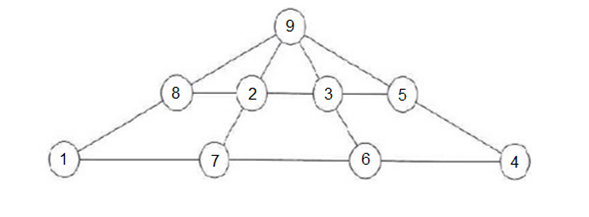
\includegraphics[scale=1]{imagenes/Combinatoria/1,2.png}
          \end{center}
          Observemos que en la figura podemos intercambiar la suma de la fila dearriba y la de abajo y las que contiene a contienen a b las podemos permutar.\\
          $\therefore$ La cantidad de formas que existen de colocar los números es $4!\cdot 2=48$ $\blacksquare$\\
          
    \item En un baile al cual asisten $n$ parejas formadas por marido y mujer se presenta la siguiente situación cuando se van a sentar a una mesa rectangular que cuenta con $2n$ sillas dispuestas en fila:
          \begin{enumerate}
              \item Cada mujer se quiere sentar al lado de su marido.
              \item Las mujeres y los hombres se quieren sentar alternadamente (entre dos hombres debe haber una mujer y entre dos mujeres debe haber un hombre).
          \end{enumerate}
          Respuesta:\\
          Analicemos el inciso (a):\\
          Como cada mujer se quiere sentar al lado de su marido podemos considerar a un hombre y una mujer que sean pareja como una sola unidad, ahora dividamos los asientos en regiones que contengan cada una dos asientos de modo que cada región sea ocupada por una pareja. Luego podemos distribuir las parejas de $(2n)!$ formas pero da lo mismo que una mujer se siente a la derecha o a la izquierda de su marido.\\
          $\therefore$ la cantidad de formas sería $2\cdot(2n)!$ $\blacksquare$\\
          Ahora solucionemos el inciso (b)\\
          Como debemos alternar entre hombres y mujeres empecemos por la izquierda de la fila a dividir los asientos en asientos de hombres y asientos de mujeres de modo que el primero sea de hombre, el segundo de mujer, el tercero de hombre y así sucesivamente, luego nos quedaremos con $n$ asientos de hombres y $n$ de mujeres, pero la cantidad de formas en que podemos sentar a los hombre en sus respectivos asientos es $n!$ al igual que para las mujeres.\\
          $\therefore$ Como podemos también hacer el proceso descrito comenzando por la derecha de la fila, la cantidad de formas sería $2{(n!)}^2$ $\blacksquare$\\
    \item Matematiquito tiene escrito en una pizarra los números del 1 al 2019. Luego en cada paso escoge dos números, los borra, los suma y escribe la suma de los dígitos del número obtenido. Puede que el último número que obtenga Matematiquito sea:
          \begin{enumerate}
              \item  El 3.
              \item El 6.
          \end{enumerate}
          Respuesta:\\
          Utilicemos el siguiente lema: sea $S(n)$ la suma de las cifras de $n$, luego $S(n)\equiv n$ (mód 9), ahora demostremos el lema:
          $$n=\overline{a_1a_2a_3\ldots a_k}$$
          \begin{center}
              $\overline{a_1a_2a_3\ldots a_k}\equiv a_1+a_2+\ldots +a_k$ (mód 9)\\
              $10^{k-1}a_1+10^{k-2}+\ldots+a_k\equiv a_1+a_2+\ldots +a_k$ (mód 9)\\
              $a_1+a_2+\ldots +a_k\equiv a_1+a_2+\ldots +a_k$ (mód 9)
          \end{center}
          Con lo que queda demostrado.\\
          Ahora observemos que cuando se realiza lo descrito en el problema, el número que se va escribiendo en la pizarra conserva la congruencia (mód 9) de la suma de los dos anteriores que lo generaron, entonces se tiene que cumplir que el último número que obtenga Matematiquito sea congruente con $1+2+3+\ldots+2019$ en el (mód 9). Por tanto comprobemos si puede ser el 3:
          \begin{center}
              $1+2+3+\ldots+2019\equiv 3$ (mód 9)\\
              $2020\cdot 2019/2\equiv 3$ (mód 9)\\
              $4\cdot 3/2\equiv 3$ (mód 9)\\
              $6\equiv 3$ (mód 9)\\
          \end{center}
          Lo cual es imposible.\\
          $\therefore$ El último número que obtenga Matematiquito no puede ser el 3$\blacksquare$\\
          Analicemos el (b).\\
          Si fuera posible encontrar el 6 solo tendremos que encontrar una configuración en la que el resultado final sea 6.\\
          Dividamos la lista de números de nueve en nueve, de modo que el primer grupo sea $\{1, 2, 3, \ldots, 9\}$ y el último sea $\{2012, 2014 ,\ldots , 2016\}$, dejando a parte al 2017, 2018 y al 2019. Ahora Matematiquito va a escoger los números de modo tal que sean del mismo grupo y que su suma sea múltiplo de 9. Pero como la mayor suma que obtendrá en este paso será $2012+2015=4027$, entonces el mayor número que escribirá en la pizarra será el 27 generado por las sumas 999 o 3555, etc ya que todos los números escritos son múltiplos de 9. Después Matematiquito escogerá los múltiplos de 9 escritos antes de este paso hará el procedimiento de 2 en 2, pero como la mayor suma que puede obtener es $2016+2011=4027$ al igual que el paso anterior el mayor número que escribirá en la pizarra será el 27 por lo que probamos anteriormente. Luego tenemos múltiplos de 9 menores e iguales que 27 y si realizamos el procedimiento con estos obtendremos como sumas: 18, 27, 36, 45 y 63, que todas generan al 9. Al final Matematiquito tendrá en la pizarra el 9, 2017, 2018 y 2019 y al realizar la operación con estos obtendremos el 6.\\
          $\therefore$ Hemos encontrado una configuración cuyo resultado es 6 $\blacksquare$\\
    \item En un país un caso policial hay $n$ sospechosos, de manera tal que cada uno conoce a los culpables, pero se sabe que los culpables fueron los únicos que dijeron mentira en los interrogatorios. Llamemos $a_i$ al sospechoso $i$. En los interrogatorios se hizo solo una pregunta: ¿cuántos culpables hay? y estas fueron las respuestas:
          \begin{center}
              $a_1$: 1 culpable.\\
              $a_2$: 2 culpables.\\
              $\vdots$\\
              $a_i: i$ culpables.\\
              $\vdots$\\
              $a_n: n$ culpables
          \end{center}
          Ayude a resolver el caso policial determinando los criminales.\\
          Respuesta:\\
          Como todos están diciendo cifras diferentes solo uno puede estar diciendo la verdad. $\therefore$ El que dice la verdad $n-1$-ésimo interrogado y los criminales son todos los demás $\blacksquare$\\
    \item Se tiene un polígono regular de $2k$ lados. ¿Qué probabilidad hay de escoger 3 vértices de este polígono y que estos formen un triángulo rectángulo?\\
          Respuesta:\\
          Inscribamos el polígono regular en una circunferencia. Luego cualquier triángulo rectángulo que formemos utilizando los vértices de este polígono por el teorema de Tales contendrá dos vértices que formarán un diámetro. Demostremos que este planteamiento es posible de lograr en nuestro polígono: si trazamos un diámetro que pase por uno de los vértices obtendremos dos semiplanos y como el diámetro es el eje de simetría de la circunferencia entonces en cada semiplano tendremos la misma cantidad de vértices, como $2k-1$ es un número impar entonces el diámetro trazado anteriormente contendrá otro de los vértices del polígono con lo cual queda demostrado.
          Ahora a la hora de calcular los casos favorables tendremos que contar la cantidad de diámetros que tiene esta circunferencia, que serían $k$, pero al escoger un diámetro podemos escoger cualquiera de los restantes $2k-2$ vértices como tercer vértice de nuestro triángulo. Entonces la cantidad de triángulos rectángulos que podemos hacer es $k(2k-2)$. Calculemos entonces el número pedido:
          $$\frac{k(2k-2)}{\frac{(2k)!}{(2k-3)!3!}}=\frac{6k(2k-2)}{2k(2k-1)(2k-2)}=\frac{3}{2k-1}$$
          $\therefore$ La probabilidad que hay de escoger 3 vértices de este polígono y que estos formen un triángulo rectángulo es $\displaystyle{\frac{3}{2k-1}}$ $\blacksquare$\\
    \item En una granja se tienen gallinas y patos en un corral de 123 x 123 unidades dividido en regiones de una unidad cuadrada y contiene un solo animal. Los animales se ubican de la siguiente forma: si una región contiene un pato(siempre que no este en el borde), la cantidad de regiones con gallinas aledañas a esta debe ser igual a 4 y si una región contiene una gallina(siempre que no este en el borde), la cantidad de regiones con patos aledañas a esta debe ser igual a 5. Halle la cantidad de gallinas y patos presentes en el corral.\\
          Respuesta:\\
          Dividamos el corral en espacios de 3 x 3 y veamos lo que ocurre en estos espacios. Si la región central contiene un pato entonces las que la rodean contendrán 4 gallinas y 4 patos, de modo que este espacio contendrá 5 patos y 4 gallinas. Por el contrario si la región del medio contiene una gallina las que la rodean contendrán 5 patos y 3 gallinas, de modo que este espacio contendrá 5 patos y 4 gallinas. En los dos casos analizados los espacios que hemos construido tendrán 5 patos y 4 gallinas. \\$\therefore$ Como el corral contiene 1681 espacios entonces contendrá 8405 patos y 6724 gallinas $\blacksquare$ \\
    \item La máquina regala monedas funciona de la siguiente manera: cuando se introduce una moneda de 25 centavos la máquina devuelve cinco monedas de 5 centavos, cuando se introduce una moneda de 5 centavos la máquina devuelve cinco monedas de 1 centavo, cuando se introduce una moneda de 1 centavo la máquina devuelve cinco monedas de 25 centavos. Diego comienza con una sola moneda de 1 centavo. Decidir si después de usar la máquina repetidas veces puede retirarse con 745 centavos o con 907 centavos y para el total que se pueda, probar cómo lo puede lograr.\\
          La única manera de aumentar el dinero que le introducimos a la máquina es con una moneda de 1 centavo devolviéndonos 125 centavos y aumentando nuestro dinero en 124 centavos. Luego de aquí deducimos que nuestro dinero solo puede aumentar de 124 en 124 centavos, entonces las cifras de dinero que podemos obtener con la máquina deben dejar resto 1 en la división por 124:
          \begin{center}
              906$\equiv$38 (mód 124)\\
              745$\equiv$1 (mód 124)
          \end{center}
          Ahora con 906 no se puede y con 745 si, demostremos como: $745=6\cdot 124+1$ esto nos indica que tenemos que introducir 6 monedas de 1 centavos, para ello echamos la primera con que comenzamos y la fraccionamos utilizando la máquina en 125 de a 1 centavo, luego cogemos 5 de estas últimas las echamos y obtendremos 625 centavos sumándole los otros 120 centavos serían 745. \\$\therefore$ Queda demostrado $\blacksquare$\\
    \item Un coche de un tren tiene dos filas enfrentadas, de 5 asientos cada una, con un asiento de cada fila junto a la ventana. Hay 9 pasajeros, tres de los cuales quieren sentarse en sentido de la marcha. A los otros 6 no les importa el sentido, pero hay una madre cuyo hijo quiere sentarse junto a ella y al lado de la ventana. ¿De cuántas maneras pueden sentarse los pasajeros de forma tal que todos estén satisfechos?\\
          Respuesta:\\
          Observemos que la mamá y el niño solo se pueden sentar de dos formas, en la fila que está en sentido de la marcha o en la otra, en ambas junto a la ventana, entonces basándonos en estos dividamos el ejercicio en dos casos.\\
          1er Caso\\
          La mamá y el niño se sientan en la fila que está en el sentido de la marcha:\\
          En esta fila solos queda espacio para los 3 pasajeros que se quieren sentar en sentido de la marcha, los cuales se pueden sentar de 3! formas. Ahora en la otra fila tenemos que sentar a los otros 4 pasajeros, pero como tenemos 5 asientos, entonces estamos en presencia de una variación: $V_{4}^{5}=5!$. Luego para este caso tenemos $3!\cdot 5!=720$ posibilidades.\\
          2do Caso\\
          La mamá y el niño se sientan en la fila que no está en el sentido de la marcha:\\
          Primero sentemos a los 3 pasajeros que se deben sentar en la otra fila, tenemos 3 personas a ubicar en 5 espacios por tanto se pueden sentar de $V_{3}^{5}=5\cdot 4\cdot 3=60$. Ahora los restantes pasajeros se pueden ubicar en cualquiera de los 3 asientos que quedan libres en esta fila y en cualquiera de los 2 que no están ocupados en la otra fila, entonces tenemos 4 persona para 5 espacios por lo que hay $V_{4}^{5}=5!$. Para este caso tenemos $60\cdot 120=7200$ posibilidades.\\
          $\therefore$ Sumando los 2 casos tenemos 7920 posibilidades de sentar a los pasajeros $\blacksquare$\\
    \item Matematiquito está jugando un juego con sus amigos de la siguiente manera, él tiene 100 sillas dispuestas sobre una fila y a enumeradas de 1 al 100, al principio todas las sillas están ocupadas por uno de sus amigos cada una, en la segunda ronda Matematiquito pasa parando a los que están sobre las sillas pares, en la tercera Matematiquito para o sienta a sus amigos en las sillas múltiplos de 3 y así repetidamente hasta la ronda 100. Al final del juego cuáles sillas quedarán ocupadas.\\
          Respuestas:\\
          Notemos que el que sentado en la silla i solo se para o se sienta cuando Matematiquito llega a un múltiplo de i y como al inicio todos estarán sentados, al final solo quedara sentados los que se encuentren en una silla cuyo número tenga un número impar de divisores, pero los únicos números que tiene un número impar de divisores son los cuadrados perfectos.\\
          $\therefore$ Al final del juego solo quedarán ocupadas las sillas que tengan cuadrados perfecto $\blacksquare$\\
    \item Matematiquito y Matematiquita juegan alternadamente, comenzando por Matematiquito, coloreando segmentos sobre la siguiente figura, formada por triangulitos equiláteros iguales:
          \begin{center}
              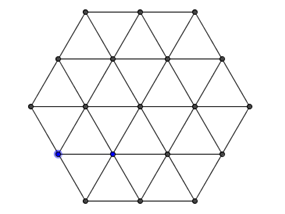
\includegraphics[scale=1]{imagenes/Combinatoria/11.png}
          \end{center}
          Las reglas del juego son las siguientes: los segmentos deben estar sobre los lados de los triangulitos, se pueden colorear los segmentos que no tengan ningún punto en común con los segmentos ya coloreados incluyendo a los extremos y por último pierde el que no pueda colorear más ningún segmento. Muestre que uno de los dos tiene una estrategia ganadora y descríbala.\\
          Respuesta:\\
          Gana Matematiquito que es el primero en empezar, en su primera jugada Matematiquito colorea cualquiera de los 3 segmentos que dividen a la figura en 2 regiones iguales:
          \begin{center}
              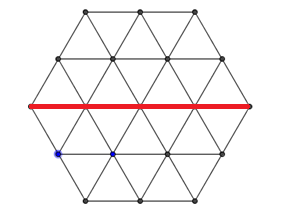
\includegraphics[scale=1]{imagenes/Combinatoria/Respuesta11.png}
          \end{center}
          Después la estrategia de Matematiquito es jugar simétrico a Matematiquita y así cada vez que esta juegue este lo podrá hacer del otro lado, pero va a existir un momento en que a Matematiquita se le acabaran los segmentos para colorear y Matematiquito ganará. \\
    \item Los números $a_1,a_2,\ldots ,a_{n^2}$ se colocan en un tablero de $n$ x $n$ de tal manera que los elementos ubicados sobre cada fila y sobre cada columna formen una progresión aritmética. Si la suma de todas las casillas del tablero es $k$. Halle la suma de los elementos ubicados en las esquinas del tablero.\\
          Respuesta:\\
          Hallemos las sumas de cada fila:
          $$a_1+a_2+\ldots+a_n=\frac{(a_1+a_n)n}{2}$$
          $$a_{n+1}+a_{n+2}+\ldots+a_{2n}=\frac{(a_{n+1}+a_{2n})n}{2}$$
          $$\vdots$$
          $$a_{n^2-n+1}+a_{n^2-n+2}+\ldots+a_{n^2}=\frac{(a_{n^2-n+1}+a_{n^2})n}{2}$$
          Sumando todas las filas tenemos:
          $$\frac{(a_1+a_n)n}{2}+\frac{(a_{n+1}+a_2n)n}{2}+\ldots+\frac{(a_{n^2-n+1}+a_{n^2})n}{2}=k$$
          $$\frac{n(a_1+a_{n+1}+a_{2n+1}+\ldots+a_{n^2-n+1})}{2}+\frac{
              n(a_n+a_{2n}+a_{3n}+\ldots+a_{n^2}}{2})=k$$
          Pero $a_1;a_{n+1};a_{2n+1};\ldots;a_{n^2-n+1}$ forman una columna, al igual que $a_n;a_{2n};a_{3n};\ldots;a_{n^2}$:
          $$\Rightarrow\frac{n^2(a_1+a_{n^2-n+1})}{4}+\frac{
              n^2(a_n+a_{n^2}}{4}=k$$
          $$a_1+a_{n^2-n+1}+a_n+a_{n^2}=\frac{4k}{n^2}$$
          $\therefore$ Ya que los elementos situados en las esquinas son $a_1;a_{n^2-n+1};a_n\wedge a_n^2$ entonces $\displaystyle{a_1+a_{n^2-n+1}+a_n+a_n^2}=\frac{4k}{n^2}$ $\blacksquare$\\
    \item Se tiene un tablero de $n$ x $n$ rellenado con los números desde el 1 hasta $n^2$, para cada fila y cada columna se calcula la diferencia entre el mayor y el menor elemento. Sea $S$ la suma de los 4096 números obtenidos. Halle el máximo valor de $S$.\\
          Respuesta:\\
          Un número puede actuar como máximo o mínimo elemento de una fila o una columna a lo sumo 2 veces, entonces para encontrar el mayor valor de $S$, debemos encontrar una configuración en la que los $n$ números más pequeños del tablero actúen 2 veces como mínimo elemento de una fila o una columna y n la que los $n$ números más grandes del tablero actúen 2 veces como máximo elemento de una fila o una columna. Para ello coloquemos los números desde el 1 hasta $n$ en una diagonal y los números desde $n^2-n+1$ hasta $n^2$ en la otra diagonal:
          $$S=2(n^2-n+1+\ldots +n^2-1-\ldots-n)$$
          $$S=2n^3-(n-1)n-n(n+1)$$
          $$S=2n^3-n^2+n-n^2-n$$
          $$S=2n^3-2n^2$$
          $\therefore$ El máximo valor de $S$ es $2n^3-2n^2$ $\blacksquare$\\
    \item Matematiquito y Matematiquita juegan alternadamente sobre la cuadricula dada. Cada uno en su turno traza de 1 a 5 recorridos diferentes a los trazados anteriormente, que unan A con B, moviéndose únicamente a la derecha y hacia arriba sobre las líneas de la cuadricula. Juan empieza jugando. Pierde el que trace un recorrido que pase por C o D. Prueba que uno de ellos puede ganar independientemente de como juegue el otro.
          \begin{center}
              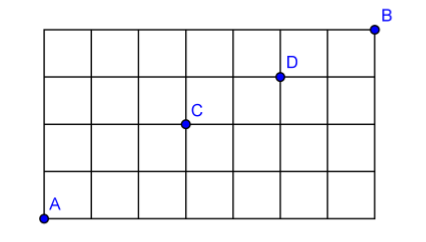
\includegraphics[scale=1]{imagenes/Combinatoria/13.png}
          \end{center}
          
          Respuesta:\\
          Calculemos la cantidad de recorridos válidos en el juego. Para ello calculemos primero la cantidad de recorridos desde A a B: observemos que para llegar desde A hasta B debemos realizar 4 movimientos hacia arriba, a los cuales denotaremos como (M) y 7 hacia la derecha a los cuales llamaremos (N). Ahora armemos un recorrido con esta notación N N M N N N M M N M N y demostrémoslo mediante un ejemplo:
          \begin{center}
              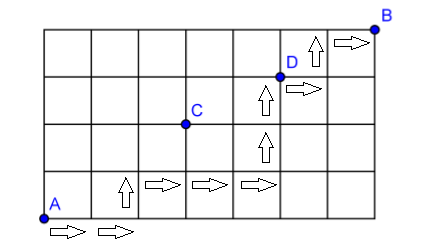
\includegraphics[scale=1]{imagenes/Combinatoria/Respuesta13.png}
          \end{center}
          Entonces nos damos cuenta que lo que hace diferente un recorrido de otro es en que orden colocamos las M y las N(el orden en que elegimos entre subir o ir hacia la derecha). Luego tenemos 11 espacios y tenemos que elegir para colocar las N lo que nos da un total de $\displaystyle{11 \choose 7}$ combinaciones y después de colocar las N, las M ocuparan los espacios que quedan vacíos, por tanto hay $\displaystyle{11 \choose 7}=330$ recorridos desde A hasta B.\\
          Calculemos los recorridos que pasan por C: para ello calculemos los caminos que llegan desde A hasta C y luego los que van desde C hasta B. Para ir de A a C tenemos que ir 2 veces hacia arriba y 3 veces hacia la derecha para un total de $\displaystyle{5 \choose 2}=10$ combinaciones, al igual que procedimos anteriormente. Para ir desde C a B tenemos que ir 2 veces hacia arriba y 4 hacia la derecha para un total $\displaystyle{6 \choose 2}=15$ combinaciones. Entonces como ir de A a C implica ir de C a B para completar los recorridos tenemos $10\cdot 15=150$ recorridos que pasan por C.\\
          Calculemos los recorridos que pasan por D: para ello calculemos los caminos que llegan desde A hasta D y luego los que van desde D hasta B. Para ir de A a D tenemos que ir 3 veces hacia arriba y 5 veces hacia la derecha para un total de $\displaystyle{8 \choose 3}=56$ combinaciones. Para ir desde D a B tenemos que ir una vez hacia arriba y 2 hacia la derecha para un total $\displaystyle{3 \choose 2}=13$ combinaciones. Entonces como ir de A a D implica ir de D a B para completar los recorridos tenemos $56\cdot 3=168$ recorridos que pasan por D.\\
          Ahora nos falta calcular los que pasan por C y D al mismo tiempo: para ello calculemos los caminos que llegan desde C a D. Para ir de C a D tenemos que ir una vez hacia arriba y 2 hacia la derecha para un total $\displaystyle{3 \choose 2}=13$ combinaciones. Entonces como ir de A a C implica ir de C a D e implica ir de D a B para completar los recorridos tenemos $10\cdot 3\cdot 3=90$ recorridos que pasan por C y D al mismo tiempo.\\
          Entonces tenemos $150+168-90=228$ recorridos que pasan por C o por D y como hay 330 recorridos en total entonces tenemos 102 recorridos válidos.\\
          Veamos otra forma de calcular los recorridos válidos: observemos que para llegar a una esquina solo podemos hacerlo mediante la que está abajo o a la izquierda de esta, entonces la cantidad de recorridos que llegan a esa esquina será la suma de la cantidad de recorridos que llegan a la que está abajo o a la izquierda de dicha esquina. Ahora apliquemos este principio:
          \begin{center}
              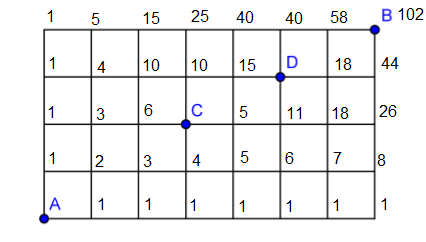
\includegraphics[scale=1]{imagenes/Combinatoria/Copia13.png}
          \end{center}
          Así mediante esta vía también obtenemos 102 recorridos válidos. Como la cantidad de recorridos válidos es múltiplo de 6 gana Matematiquita con la siguiente estrategia: cuando Matematiquito trace sus recorridos, Matematiquita trazará una cantidad de recorridos de modo que la cantidad de caminos que queden sea múltiplo de 6 esto siempre se puede lograr ya que la cantidad de recorridos en cada jugada es menor a 6. \\
          $\therefore$ De este modo al final quedarán 6 caminos por trazar y le tocará jugar a Matematiquito, luego este siempre dejará al menos un recorrido sin hacer y en la próxima jugada Matematiquita ganará $\blacksquare$\\
    \item Matematiquito y Matematiquita inician un juego donde alternadamente van sustituyendo el número escrito en la pizarra. En cada turno, el jugador debe sustituir el número escrito, ya sea por la cantidad de divisores del número escrito o por la diferencia entre el número escrito y su cantidad de divisores. Matematiquito es el primero en jugar, y el que escriba el cero gana. Dado que el número inicial es 1036, determine qué jugador tiene una estrategia ganadora y enúnciela.\\
          Respuesta:\\
          Notemos que 1036 tiene 12 divisores, entonces Matematiquito puede escribir 12 ó 1024:\\
          Caso 1\\
          Matematiquito escribe 12: ya que 12 tiene 6 divisores Matematiquita solo puede jugar 6. Ahora 6 tiene 4 divisores, entonces Matematiquito puede escribir 2 ó 4, pero si juega 2 Matematiquita en la otra jugada ganará, así que escribe el 4. Matematiquita no puede escribir el 1 porque si lo hace en la otra jugada Matematiquito ganará, por lo que escribe el 3. Entonces Matematiquito puede escribir el 2 o el 1 pero en cualquiera de los 2 casos Matematiquita ganará. \\
          Caso 2\\
          Matematiquito escribe 1024: pero aquí Matematiquita deberá jugar 11 y Matematiquito se verá obligado a jugar 9 porque si escribe el 2 pierde. Entonces Matematiquita puede jugar 3 ó 6, pero como vimos anteriormente con cualquiera de estos 2 números Matematiquita ganará.\\
          $\therefore$ Juegue como juegue Matematiquito, Matematiquita siempre ganará $\blacksquare$\\
    \item En la pizarra está escrito el número 3. Matematiquito y Matematiquita juegan alternadamente, comenzando Matematiquito, de la manera siguiente: si en la pizarra está escrito el número $n$, el jugador que tenga el turno lo debe sustituir por cualquier entero $m$ que sea primo relativo con $n$ y tal que $n<m<n^2$. El primer jugador que escriba un número mayor o igual a 2016 gana. Determine qué jugador tiene una estrategia ganadora y enúnciela.
          \\Respuesta:\\
          Notemos que $44^2<2016<45^2$, entonces el jugador que escriba el 44 obligará al otro a jugar un número mayor que 44 pero menor que 2016 y en la próxima jugada el que escribió el 44 ganará. Ahora como $44=4\cdot 11$ para poder jugar el 44 debe haber escrito un número impar mayor que 7 y diferente de 11. El primer jugador puede jugar: 4, 5, 7 ó 8, si juega el 7, el segundo ganará; pero si juega el 8 obligará al segundo a jugar un número impar mayor que 7, el segundo para no perder se verá obligado a jugar el 11 porque de lo contrario cualquier otro número le permitirá al primero poder jugar el 44 y ganar. Luego es turno del primero y este jugará cualquier número par mayor que 12 pero menor que 44, para obligar al segundo a jugar un número impar mayor que 11, entonces si este último juega un número menor que 44, el primero jugará el 44 y ganará y si juega un número mayor a 44 entonces igualmente el primero ganará.\\
          $\therefore$ Matematiquito ganará independientemente de como juegue Matematiquita $\blacksquare$\\
    \item Un conjunto $X$ de enteros positivos es ibérico si $X$ es un subconjunto de {2,3,4,...,3141592653589} y siempre que $m$ y $n$ pertenezcan a $X$, entonces el $mcd(m;n)$ pertenece también a $X$. Un conjunto ibérico es olímpico si no está contenido en ningún otro conjunto ibérico. Encontrar todos los conjuntos ibéricos olímpicos que contienen el número 33.\\
          Respuesta:\\
          $33=3\cdot 11$, ahora supongamos que $3k$ y $11m$ también están en $X$, de modo tal que $mcd(k;11)=1\wedge mcd(m;3)=1\Rightarrow mcd(3k;11m)=1$ lo cual es una contradicción, esto nos dice que $k=11a\vee m=3b$ con $a$ y $b$ enteros positivos. Entonces para que $X$ sea ibérico y $33\in X$ todos los elementos de $X$ tienen que ser todos múltiplos de 3 ó todos múltiplos de 11 ó todos múltiplos de 33.\\
          Ahora percatémonos que si tenemos un número $n$ primo, entonces el conjunto de todos los múltiplos de $n$, al cual denotaremos $X_n$ será ibérico, ya que $mcd(ny;nz)=nk$ y $nk\in X_n$, pero además $X_n$ es olímpico, porque si le agregamos más elementos estos no tendrían factores en común con $n$, ya que $n$ es primo y no hay más múltiplos de $n$, por tanto el conjunto dejaría de ser ibérico.\\
          Entonces $33=3\cdot 11\Rightarrow 33\in X_3\wedge 33\in X_{11}$, además $33\in X_{33}$ ya que $X_{33}\subset X_3\wedge X_{33}\subset X_{11}$, luego $X_{33}$ no es olímpico.\\
          $\therefore$ Los conjuntos ibéricos olímpicos que contienen el número 33 son $X_3$ y $X_{11}$ $\blacksquare$\\
    \item Sea $n$ un entero positivo. Para una permutación $a_1,a_2,\ldots ,a_n$ de los números $1,2,\ldots ,n$ , definimos:
          
          $$b_k=\min_{1\leq i\leq k}a_i+\max_{1\leq j\leq k} a_j$$
          para cada $k = 1,2,\ldots ,n$. \\
          Decimos que la permutación $a_1,a_2,\ldots ,a_n$ es guadiana si la sucesión $b_1,b_2,\ldots ,b_n$ no tiene dos elementos consecutivos iguales. ¿Cuántas permutaciones guadianas existen?    \\
          Respuesta:\\
          Notemos que para que la permutación sea guaniana se debe cumplir que:
          $$b_k\neq b_{k+1}\Rightarrow \min_{1\leq i\leq k}a_i+\max_{1\leq j\leq k} a_j\neq \min_{1\leq i\leq k+1}a_i+\max_{1\leq j\leq k+1} a_j\Rightarrow a_{k+1}<\min_{1\leq i\leq k}a_i\vee a_{k+1}>\max_{1\leq j\leq k} a_j$$
          Ahora supongamos que $\min_{1\leq i\leq k}a_i=a_m$, entonces por lo anterior planteado: $$\min_{1\leq i\leq k}a_i>b_{m+1}\vee a_{m+1}>\max_{1\leq j\leq m} a_j$$ Para la primera posibilidad tenemos que: $m+1>k\Rightarrow k=m$ ya que por lo antes definido no puede haber otro número entre $a_1$ y $a_k$ que sea menor que $a_m$. Para la otra posibilidad tenemos que $b_{m+1}>\max_{1\leq j\leq m} a_j$, ahora si seguimos avanzando para $a_{m+2},a_{m+3},\ldots, a_k$, cada uno será mayor que el anterior ya que $\min_{1\leq i\leq k}a_i=a_m$, por lo que $a_k>a_{k-1}>\ldots>a_{m+1}>\max_{1\leq j\leq m} a_j\Rightarrow a_k=\max_{1\leq j\leq k} a_j$. De estas 2 variantes concluimos que:
          $$a_k=\max_{1\leq j\leq k} a_j\vee a_k=\min_{1\leq i\leq k}a_i$$
          
          Ahora demostremos que usando esta configuración podemos obtener una permutación guaniana. Digamos que:
          $$b_x=\min_{1\leq i\leq x}a_i+\max_{1\leq j\leq x} a_j$$
          $$b_{x+1}=\min_{1\leq i\leq x+1}a_i+\max_{1\leq j\leq x+1} a_j$$
          Luego tenemos 2 variantes $a_{x+1}=\max_{1\leq j\leq x} a_j\vee a_{x+1}=\min_{1\leq i\leq x+1}a_i$. \\
          Para $a_{x+1}=\max_{1\leq j\leq x} a_j\Rightarrow \min_{1\leq i\leq x}a_i=\min_{1\leq i\leq x+1}a_i\wedge a_{x+1}>\max_{1\leq j\leq x} a_j\Rightarrow b_{x+1}\neq b_{x}$, con lo que queda demostrado.\\
          Para $a_{x+1}=\min_{1\leq j\leq x} a_j\Rightarrow \max_{1\leq i\leq x}a_i=\max_{1\leq i\leq x+1}a_i\wedge a_{x+1}<\min_{1\leq j\leq x} a_j\Rightarrow b_{x+1}\neq b_{x}$, con lo que queda demostrado.\\
          Entonces para $a_n$ tenemos dos variantes 1 ó $n$, para $a_{n-1}$ también tenemos 2 posibilidades $\max_{1\leq j\leq n-1} a_j\vee a_k=\min_{1\leq i\leq n-1}a_i$, que pueden ser 1 si este no se usó para $a_n$ y $n-1$ y  $n$, si este no se usó para $a_n$ y 2. De esta manera para cada $a_k$, tenemos 2 posibilidades hasta llegar a $a_1$, donde solo nos queda una posibilidad. \\
          $\therefore$ Existen $2^{n-1}$ permutaciones guadianas $\blacksquare$\\
    \item Se tiene un polígono regular $P$ con $2n+1$ vértices y en cada vértice hay un caramelo. Dos jugadores Matematiquita y Matematiquito van a jugar alternadamente empezando por Matematiquita, con las siguientes reglas. Primero Matematiquita elige un triángulo con vértices en $P$ y coloca en el interior del triángulo el número 1, después Matematiquito elige un triángulo con vértices en $P$ y coloca en el interior del triángulo el número 2, de tal forma que los triángulos elegidos en cada jugada no se intersecan en su interior con los anteriores. Continúan así hasta que no pueden realizar más jugadas. Después el caramelo que hay en cada vértice lo gana el jugador que tenga más triángulos con su número incidiendo en ese vértice, si la cantidad de triángulos incidentes en un vértice es la misma para los dos jugadores el caramelo no se lo lleva nadie y sale del juego. Gana el jugador que más caramelos acumule. Determine el jugador que siempre puede lograr la victoria y describa su estrategia.\\
          Nota: Los triángulos pueden compartir lados y vértices.\\
          Respuesta:\\
          Tracemos una recta por uno y solo uno de los vértices del polígono de modo que a cada lado de la recta halla la misma cantidad de vértices, dividiendo al polígono en 2 regiones a las cuales llamaremos $r_a$ y $r_b$. Ahora observemos que Matematiquita puede empezar eligiendo el triángulo formado por el vértice contenido en la recta, el que está más cerca de la recta en vértice $r_a$ y el que está más cerca de la recta en vértice $r_b$, ahora cuando Matematiquito escoja su triángulo, Matematiquita deberá jugar simétrico a este, de modo que al final del juego cuando no existan más jugadas permisibles si Matematiquito gana un caramelo en una región, Matematiquita lo habrá ganado en la otra. Entonces a la hora de contar los caramelos de cada región los 2 jugadores tendrán la misma cantidad pero nos falta el caramelo que se encuentra sobre el vértice contenido en la recta: si Matematiquito tiene $n$ triángulos incidiendo en $r_a$ entonces Matematiquia tendrá $n$ triángulos incidiendo en $r_b$, si Matematiquito tiene $m$ triángulos incidiendo en $r_b$ entonces Matematiquia tendrá $m$ triángulos incidiendo en $r_a$, de modo que cada jugador tiene la misma cantidad de triángulos contenidos en las regiones incidiendo sobre ese vértice, pero el primer triángulo que escogió Matematiquia está en ambas regiones, luego el caramelo en disputa es de Matematiquita.\\
          $\therefore$ Hemos demostrado que Matematiquia siempre puede obtener un caramelo más, independientemente de como juegue Matematiquio $\blacksquare$\\
    \item Un polígono regular de $n$ lados $(n\geq 3)$ tiene sus vértices enumerados del 1 al $n$. Se dibujan todas las diagonales del polígono. Demuestre que si $n$ es impar, es posible asignar a cada lado y a cada diagonal un número entero entre 1 y $n$, de modo que cumplan las siguientes condiciones:
          \begin{enumerate}
              \item El número asignado a cada lado o diagonal es diferente al número asignado a cada uno de los 2 vértices que están en sus extremos.
              \item El número asignado a cada vértices es diferente al número asignado a cada uno de los lados o diagonales los que contienen a este vértice.
          \end{enumerate}
          Respuesta:\\
          Inscribamos el polígono en una circunferencia, ahora escojamos un vértice con un número $m$ con $1\leq m\leq n$, tracemos un diámetro por dicho vértice, entonces como el polígono es regular y $n$ impar, el diámetro trazado será la mediatriz de $\displaystyle{{n-3 \over 2}}$ diagonales y de un lado y a estos segmentos pongámosle el número $m$, de esta manera ningún segmento de los mencionados contendrá al vértice que tiene el número $m$. Seguimos de esta manera con los restantes vértices.\\
          $\therefore$ Mediante esta configuarción es posible completar el polígono cumpliendo con las condiciones del ejercicio $\blacksquare$\\
    \item Se distribuyen 2020 puntos en una circunferencia Matematiquita y Matematiquita están jugando de la siguiente manera comenzando por Matematiquita, en cada turno un jugador elige 2 puntos y los une mediante un segmento, el juego termina cuando todos los puntos sean elegidos al menos una vez y gana el jugador que realice la última jugada. Uno de los 2 jugadores tiene una estrategia ganadora, describa dicha estrategia.\\
          Respuesta:\\
          Como en cada jugada solo se pueden unir uno o 2 puntos que no hayan sido elegido antes, entonces al final del juego quedaran 4 ó 3 puntos por escoger, si quedan 4 el jugador que le toque no podrá elegir 2 porque si no el otro ganará, luego podemos asegurar que siempre quedarán 3 puntos por escoger. Ahora tenemos 2020 puntos seleccionados y se nos presentan 2 casos:\\
          Caso 1\\
          El que hizo la última jugada cuando fue Matematiquita: entonces habrá una cantidad impar de segmentos. De aquí en adelante el que juegue unirá 2 de los puntos que ya han sido escogidos porque si escoge uno o 2 de los que no han sido escogidos en la próxima jugada el otro jugador ganará, pero como la cantidad de segmentos que se pueden trazar sin elegir los 3 últimos puntos es $\displaystyle{{2017 \choose 2}={2017\cdot 2019\over 2}}$ que es un número par, nos faltarían por trazar una cantidad impar de segmentos para poder realizar este procedimiento, el cual empezará Matematiquito y lo concluirá él ya que la cantidad de jugadas es impar. Después Matematiquita se verá obligada escoger cualquiera de los puntos no seleccionados anteriormente y Matematiquito ganará.\\
          Caso 2\\
          El que hizo la última jugada cuando fue Matematiquito: entonces habrá una cantidad par de segmentos. De aquí en adelante el que juegue unirá 2 de los puntos que ya han sido escogidos porque si escoge uno o 2 de los que no han sido escogidos en la próxima jugada el otro jugador ganará, pero como la cantidad de segmentos que se pueden trazar sin elegir los 3 últimos puntos es $\displaystyle{{2017 \choose 2}={2017\cdot 2019\over 2}}$ que es un número par, nos faltarían por trazar una cantidad par de segmentos para poder realizar este procedimiento, el cual empezará Matematiquita y lo concluirá Matematiquito ya que la cantidad de jugadas es par. Después Matematiquita se verá obligada escoger cualquiera de los puntos no seleccionados anteriormente y Matematiquito ganará.\\
          $\therefore$ Matematiquito siempre podrá garantizar la victoria $\blacksquare$\\
    \item  Sea la función $f(x)$ de $\R\rightarrow\Z$ tal que:
          $$f(x)=\bigg[\frac{x+1}{2}\bigg]+\bigg[\frac{x+2}{2}\bigg]+\bigg[\frac{x+3}{2}\bigg]$$
          Halle el área que ocupa en el plano carteciano los pares reales $(x;y)$ tales que $f(x)+f(y)$ es divisible por 3, $0\leq x\leq\pi$ y $0\leq y\leq \pi$.
          $f(x)=[x]$ se interpreta como parte entera de $x$.\\
          Respuesta:\\
          Descompongamos los sumandos convenientemente:
          $$f(x)=\bigg[{x\over 2}+{1\over 2}\bigg]+\bigg[{x\over 2}+1\bigg]+\bigg[{x\over 2}+1+{1\over 2}\bigg]$$
          $$\Rightarrow f(x)=\bigg[{x\over 2}+{1\over 2}\bigg]+1+\bigg[{x\over 2}\bigg]+\bigg[{x\over 2}+{1\over 2}\bigg]+1$$
          $$f(x)=2\cdot\bigg[{x\over 2}+{1\over 2}\bigg]+2+\bigg[{x\over 2}\bigg]$$
          Nótese que si la cifra de las unidades de $x$ es impar entonces:
          $$\bigg|\bigg\{{x\over 2}\bigg\}\bigg|>0.5$$
          Denotándose $\{x\}$ como parte fraccionaria de $x$. Ahora demostremos lo que planteamos anteriormente.
          $$|x|=|[x]|+|\{x\}|$$
          Sustituyendo:
          $$\bigg|\bigg\{{x\over 2}\bigg\}\bigg|=\bigg\{{|x|\over 2}\bigg\}$$
          $$\bigg|\bigg\{{x\over 2}\bigg\}\bigg|=\bigg\{\frac{|[x]|+|\{x\}|}{2}\bigg\}$$
          $$\bigg|\bigg\{{x\over 2}\bigg\}\bigg|=\bigg\{\frac{|[x]|-1+1+|\{x\}|}{2}\bigg\}$$
          $$\bigg|\bigg\{{x\over 2}\bigg\}\bigg|=\bigg\{\frac{|\{x\}|}{2}+{1\over 2}\bigg\}$$
          Pero como $|\{x\}|<1$ entonces se cumple que:
          $$\frac{|\{x\}|}{2}<\frac{1}{2}$$
          $$\Rightarrow {|\{x\}|\over 2}+{1\over 2}<1$$
          Luego de aquí se obtiene que:
          $$\bigg|\bigg\{{x\over 2}\bigg\}\bigg|=\bigg\{\frac{|\{x\}|}{2}+{1\over 2}\bigg\}=\bigg\{\frac{|\{x\}|}{2}\bigg\}+{1\over 2}$$
          Por tanto queda demostrado. Ahora demostremos que si la cifra de las unidades de $x$ es par entonces:
          $$\bigg|\bigg\{{x\over 2}\bigg\}\bigg|<0.5$$
          $$\bigg|\bigg\{{x\over 2}\bigg\}\bigg|=\bigg\{\frac{|[x]|+|\{x\}|}{2}\bigg\}$$
          $$\Rightarrow \bigg|\bigg\{{x\over 2}\bigg\}\bigg|=\bigg\{{|\{x\}|\over 2}\bigg\}$$
          Pero anteriormente habíamos demostrado que:
          $$\frac{|\{x\}|}{2}<\frac{1}{2}$$
          Con lo cual queda demostrado.\\
          1er Caso \\
          La cifra de las unidades de $x$ es par.
          $$\Rightarrow\bigg[{x\over 2}+{1\over 2}\bigg]=\bigg[{x\over 2}\bigg]$$
          $$f(x)=3\cdot\bigg[{x\over 2}\bigg]+2$$
          2do Caso\\
          La cifra de las unidades de $x$ es impar.
          $$\Rightarrow\bigg[{x\over 2}+{1\over 2}\bigg]=\bigg[{x\over 2}\bigg]+1$$
          $$f(x)=3\cdot\bigg[{x\over 2}\bigg]+4$$
          Ahora si escogiéramos los pares ordenados solamente de un caso no se cumpliría por tanto se debe escoger para que se cumpla una $x$ del 1ro y una $y$ del 2do o una $x$ del 2do y una $y$ del 1ro. \\
          $\therefore$ De esta manera ocuparíamos un área de $\displaystyle{\pi^2\over 2}$ unidades cuadradas $\blacksquare$\\
    \item Sea $n>1$ un entero positivo, Matematiquito tiene $n$ casillas sobre una pizarra enumeradas des 1 hasta $n$, Matematiquita escribió dentro de cada casilla un único número de tal forma que al finalizar la pizarra solo contenía varias cantidades de los números 2019 o 6057. Entonces Matematiquito calculó el producto de todos los números escritos en las casillas. ¿De cuántas maneras Matematiquita puede hacer su labor para que el producto calculado sea un cuadrado perfecto.\\
          Respuesta:\\
          Descompongamos los números en factores primos: $2019=3\cdot 673$ $6057=3^2\cdot 673$. Sea $P$ el producto de todos los números y $a$ la cantidad de casillas donde está el 2019 $P=3^{2(n-a)+a}\cdot  673^{n}\Rightarrow 2n-a=2k \wedge n=2m$, luego $a$ y $n$ son pares. Ahora la cantidad de formas que hay de calcular $P$ depende de la cantidad de casillas que tienen al 2019, es decir de $a$, entonces podemos escoger $2m$ casillas para poner el 2019, pero también podemos escoger $2m-2$ casillas, $2m-4$, $\ldots$, 2, 0 casillas. De esta forma la cantidad de maneras en la que Matematiquito puede lograr que $P$ sea un cuadrado perfecto es:
          $${2m \choose 2m}+{2m \choose 2m-2}+{n \choose 2m-4}+\ldots+{2m \choose 2}+{2m \choose 0}$$
          Probemos la siguiente identidad:
          $${a+1 \choose b+1}={a \choose b}+{a \choose b+1}$$
          $${(a+1)!\over (a-b)!(b+1)!}={a!\over (a-b)!b!}+{a!\over (a-b-1)!(b+1)!}$$
          $${(a+1)!\over (a-b)!(b+1)!}=\frac{a!b+a!+a!a-a!b}{(a-b)!(b+1)!}$$
          $${(a+1)!\over (a-b)!(b+1)!}={(a+1)!\over (a-b)!(b+1)!}$$
          Con lo cual queda probada.
          $$\Rightarrow {2m \choose 2m}={2m-1 \choose 2m-1}+{2m-1 \choose 2m}$$
          $$\Rightarrow {2m \choose 2m-2}={2m-1 \choose 2m-3}+{2m-1 \choose 2m-2}$$
          $$\vdots$$
          $$\Rightarrow {2m \choose 2}={2m-1 \choose 1}+{2m-1 \choose 2}$$
          $$\Rightarrow{2m \choose 0}={2m-1 \choose 0}$$
          $$\Rightarrow {2m \choose 2m}+{2m \choose 2m-2}+{n \choose 2m-4}+\ldots+{2m \choose 2}+{2m \choose 0}={2m-1 \choose 2m}+{2m-1 \choose 2m-1}+\ldots +{2m-1 \choose 1}+{2m-1 \choose 0}$$
          $$\Rightarrow {2m \choose 2m}+{2m \choose 2m-2}+{n \choose 2m-4}+\ldots+{2m \choose 2}+{2m \choose 0}=2^{2m-1}$$
          $\therefore$ Matematiquita puede hacer su labor de $2^{2m-1}$ maneras distintas $\blacksquare$\\
    \item Se tiene una lista con los números desde el 1 hasta el 2020 en orden ascendente Matematiquito borra los números que están en la posiciones $3n+1$, luego escribe la nueva lista y realiza el mismo procedimiento con las posiciones de la nueva lista. Matematiquito continua de esta manera hasta que queda un solo número, ¿cuál será dicho número?\\
          Respuesta:\\
          Llamemos $x$ a la cantidad de números que hay delante de un número $n$. En cada jugada $x$ se ve afectada de la siguiente manera.\\
          Caso 1\\
          $x=3k+1$, cuando se realice el procedimiento se borrarán $k+1$ números y quedarán $2k$ números.\\
          Caso 2\\
          $x=3k+2$, cuando se realice el procedimiento se borrarán $k+1$ números y quedarán $2k+1$ números.\\
          Ahora realicemos el proceso inverso, al final cuando solo que un número $x=0\Rightarrow 0=2k\Rightarrow 0=k$ por lo que antes de no haber ningún número hubo $3k+1\Rightarrow 3\cdot 0+1=1$ número, entonces ahora $x=1$. Continuemos de esta manera y llamemos $x_i$ a las $x$ que vamos obteniendo de esta manera:
          $$x_0=1\Rightarrow 1=2k+1\Rightarrow k=0\Rightarrow 3\cdot 0+2=2\Rightarrow x_1=2$$
          $$x_1=2\Rightarrow 2=2k\Rightarrow k=1\Rightarrow 3\cdot 1+1=4\Rightarrow x_2=4$$
          $$x_2=4\Rightarrow 4=2k\Rightarrow k=2\Rightarrow 3\cdot 2+1=7\Rightarrow x_3=7$$
          $$x_3=7\Rightarrow 7=2k+1\Rightarrow k=3\Rightarrow 3\cdot 3+2=2\Rightarrow x_4=11$$
          $$x_4=11\Rightarrow 11=2k+1\Rightarrow k=5\Rightarrow 3\cdot 5+2=2\Rightarrow x_5=17$$
          $$x_5=17\Rightarrow 17=2k+1\Rightarrow K=8\Rightarrow 3\cdot 8+2=2\Rightarrow x_6=26$$
          $$x_6=26\Rightarrow 26=2k\Rightarrow k=13\Rightarrow 3\cdot 13+1=40\Rightarrow x_7=40$$
          $$x_7=40\Rightarrow 40=2k\Rightarrow k=20\Rightarrow 3\cdot 20+1=61\Rightarrow x_8=61$$
          $$x_8=61\Rightarrow 61=2k+1\Rightarrow k=30\Rightarrow 3\cdot 30+2=92\Rightarrow x_9=92$$
          $$x_9=92\Rightarrow 92=2k\Rightarrow k=46\Rightarrow 3\cdot 46+1=139\Rightarrow x_10=139$$
          $$x_{10}=139\Rightarrow 139=2k+1\Rightarrow k=69\Rightarrow 3\cdot 69+2=209\Rightarrow x_{11}=209$$
          $$x_{11}=209\Rightarrow 209=2k+1\Rightarrow k=104\Rightarrow 3\cdot 104+2=314\Rightarrow x_{12}=314$$
          $$x_{12}=314\Rightarrow 314=2k\Rightarrow k=157\Rightarrow 3\cdot 157+1=472\Rightarrow x_{13}=472$$
          $$x_{13}=472\Rightarrow 472=2k\Rightarrow k=236\Rightarrow 3\cdot 236+1=709\Rightarrow x_{14}=709$$
          $$x_{14}=709\Rightarrow 709=2k+1\Rightarrow k=354\Rightarrow 3\cdot 354+2=1064\Rightarrow x_{15}=1064$$
          $$x_{15}=1064\Rightarrow 1064=2k\Rightarrow k=532\Rightarrow 3\cdot 532+1=1597\Rightarrow x_{16}=1597$$
          $$x_{16}=1597\Rightarrow 1597=2k+1\Rightarrow k=798\Rightarrow 3\cdot 798+2=2396\Rightarrow x_{17}=2396$$
          Pero 2396>2020, luego observemos que para eliminar el número $x_i+1$ son necesarias $i+2$ operaciones, porque para que $x_i$ sea igual a 0 se necesitan $i+2$ operaciones. \\
          $\therefore$ El último número será 1598 $\blacksquare$\\
    \item Matematiquito tiene el conjunto $S={1;2;3;4;\ldots ;n}$, él escoge un subconjunto no nulo de $S$, calcula el promedio de su máximo y su mínimo elemento y escribe este número en una pizarra. Al terminar con todos los subconjuntos de $S$, Matematiquito se pregunta ¿cuál será el promedio de todos los números escritos en la pizarra?\\
          Respuesta:\\
          Primero demostremos el siguiente lema: sea $b$ la cantidad de elementos de un conjunto $A$, entonces la cantidad de subconjuntos diferentes que podemos formar de $A$ es $2^b$\\
          Podemos elegir formar un subconjunto de 0 elementos, luego la cantidad de formas serían  $\displaystyle{b \choose 0}$\\
          Podemos elegir formar un subconjunto de 1 elementos, luego la cantidad de formas serían  $\displaystyle{b \choose 1}$\\
          Podemos elegir formar un subconjunto de 2 elementos, luego la cantidad de formas serían  $\displaystyle{b \choose 2}$\\
          $$\vdots$$
          Podemos elegir formar un subconjunto de $b-1$ elementos, luego la cantidad de formas ser[ian  $\displaystyle{b \choose {b-1}}$\\
          Podemos elegir formar un subconjunto de $b$ elementos, luego la cantidad de formas ser[ian  $\displaystyle{b \choose b}$\\
          Sumando todo esto tenemos:
          $${b \choose 0}+{b \choose 1}+{b \choose 2}+\ldots +{b \choose {b-1}}+{b \choose b}$$
          $$1^b {b \choose 0}+1^{b-1} {b \choose 1}+1^{b-2} {b \choose 2}+\ldots +1^1 {b \choose {b-1}}+1^0 {b \choose b}$$
          Aplicando el binomio de Newtón tememos:
          $$1^b {b \choose 0}+1^{b-1} {b \choose 1}+1^{b-2} {b \choose 2}+\ldots +1^1 {b \choose {b-1}}+1^0 {b \choose b}={(1+1)}^b=2^b$$
          Con lo cual queda demostrado.\\
          Ahora supongamos que $1\leq c\leq n$, con $c\in \N$ y calculemos la cantidad de subconjuntos donde actúa $c$ como el menor elemento, luego serían todos los que no contengan a los elementos del conjunto ${1;2;\ldots;c-1}$ ya que contiene a los únicos elementos menores que $c$ en $S$, entonces el número buscado será la cantidad de subconjuntos que podemos formar del conjunto ${c+1;c+2\ldots ,n}$, cuenta con $n-c$ elementos, lo que nos da $2^{n-c+1}$. Entonces uno de los sumando buscados para calcular el promedio final es ${2^{n-c}c\over 2}$\\
          Supongamos que $1\leq d\leq n$, con $d\in \N$ y calculemos la cantidad de subconjuntos donde actúa $d$ como el mayor elemento, luego serían todos los que no contengan a los elementos del conjunto ${d+1;d+2;\ldots;n}$ ya que contiene a los únicos elementos mayores que $d$ en $S$, entonces el número buscado será la cantidad de subconjuntos que podemos formar del conjunto ${1;2;\ldots ,d-1}$, cuenta con $d-1$ elementos, lo que nos da $2^{d-1}$. Entonces uno de los sumando buscados para calcular el promedio final es ${2^{d-1}d\over 2}$\\
          Luego apliquemos estos 2 procedimientos con todos los elementos del conjunto y así encontraremos la cantidad de subconjuntos donde actúa cada número como el mayor y el menor elemento del subconjunto respectivamente y al sumar la multiplicación de cada número por la cantidad de subconjuntos donde este actúa como el mayor y el menor elemento del subconjunto respectivamente, obtendremos el promedio buscado, al dividir esta suma entre la cantidad de subconjuntos no nulos de $S$:
          $$\frac{{2^{n-1}\cdot 1\over 2}+{2^{n-2}\cdot 2\over 2}+\ldots+{2^{n-n}\cdot n\over 2}+{2^{1-1}\cdot 1\over 2}+{2^{2-1}\cdot 2\over 2}+\ldots+{2^{n-1}\cdot n\over 2}}{2^n-1}$$
          $$\frac{{2^{n-1}\cdot 1\over 2}+{2^{n-2}\cdot 2\over 2}+\ldots+{2^{n-n}\cdot n\over 2}+{2^{1-1}\cdot 1\over 2}+{2^{2-1}\cdot 2\over 2}+\ldots+{2^{n-1}\cdot n\over 2}}{2^n-1}=\frac{{(n+1)2^{n-1}\over 2}+{(n+1)2^{n-2}\over 2}+\ldots+{(n+1)2^{n-n}\over 2}}{2^n-1}$$
          $$\frac{{2^{n-1}\cdot 1\over 2}+{2^{n-2}\cdot 2\over 2}+\ldots+{2^{n-n}\cdot n\over 2}+{2^{1-1}\cdot 1\over 2}+{2^{2-1}\cdot 2\over 2}+\ldots+{2^{n-1}\cdot n\over 2}}{2^n-1}=\frac{(n+1)(2^{n-1}+2^{n-2}+\ldots+1)}{2(2-1)(2^{n-1}+2^{n-2}+\ldots+1)}$$
          $$\frac{{2^{n-1}\cdot 1\over 2}+{2^{n-2}\cdot 2\over 2}+\ldots+{2^{n-n}\cdot n\over 2}+{2^{1-1}\cdot 1\over 2}+{2^{2-1}\cdot 2\over 2}+\ldots+{2^{n-1}\cdot n\over 2}}{2^n-1}={n+1 \over 2}$$
          $\therefore$ El promedio de todos los números escritos en la pizarra será $\displaystyle{{n+1 \over 2}}$ $\blacksquare$\\
\end{enumerate}

\end{document}

